% Options for packages loaded elsewhere
\PassOptionsToPackage{unicode}{hyperref}
\PassOptionsToPackage{hyphens}{url}
%
\documentclass[
  b5paper]{book}
\usepackage{amsmath,amssymb}
\usepackage{iftex}
\ifPDFTeX
  \usepackage[T1]{fontenc}
  \usepackage[utf8]{inputenc}
  \usepackage{textcomp} % provide euro and other symbols
\else % if luatex or xetex
  \usepackage{unicode-math} % this also loads fontspec
  \defaultfontfeatures{Scale=MatchLowercase}
  \defaultfontfeatures[\rmfamily]{Ligatures=TeX,Scale=1}
\fi
\usepackage{lmodern}
\ifPDFTeX\else
  % xetex/luatex font selection
\fi
% Use upquote if available, for straight quotes in verbatim environments
\IfFileExists{upquote.sty}{\usepackage{upquote}}{}
\IfFileExists{microtype.sty}{% use microtype if available
  \usepackage[]{microtype}
  \UseMicrotypeSet[protrusion]{basicmath} % disable protrusion for tt fonts
}{}
\makeatletter
\@ifundefined{KOMAClassName}{% if non-KOMA class
  \IfFileExists{parskip.sty}{%
    \usepackage{parskip}
  }{% else
    \setlength{\parindent}{0pt}
    \setlength{\parskip}{6pt plus 2pt minus 1pt}}
}{% if KOMA class
  \KOMAoptions{parskip=half}}
\makeatother
\usepackage{xcolor}
\usepackage{color}
\usepackage{fancyvrb}
\newcommand{\VerbBar}{|}
\newcommand{\VERB}{\Verb[commandchars=\\\{\}]}
\DefineVerbatimEnvironment{Highlighting}{Verbatim}{commandchars=\\\{\}}
% Add ',fontsize=\small' for more characters per line
\usepackage{framed}
\definecolor{shadecolor}{RGB}{248,248,248}
\newenvironment{Shaded}{\begin{snugshade}}{\end{snugshade}}
\newcommand{\AlertTok}[1]{\textcolor[rgb]{0.94,0.16,0.16}{#1}}
\newcommand{\AnnotationTok}[1]{\textcolor[rgb]{0.56,0.35,0.01}{\textbf{\textit{#1}}}}
\newcommand{\AttributeTok}[1]{\textcolor[rgb]{0.13,0.29,0.53}{#1}}
\newcommand{\BaseNTok}[1]{\textcolor[rgb]{0.00,0.00,0.81}{#1}}
\newcommand{\BuiltInTok}[1]{#1}
\newcommand{\CharTok}[1]{\textcolor[rgb]{0.31,0.60,0.02}{#1}}
\newcommand{\CommentTok}[1]{\textcolor[rgb]{0.56,0.35,0.01}{\textit{#1}}}
\newcommand{\CommentVarTok}[1]{\textcolor[rgb]{0.56,0.35,0.01}{\textbf{\textit{#1}}}}
\newcommand{\ConstantTok}[1]{\textcolor[rgb]{0.56,0.35,0.01}{#1}}
\newcommand{\ControlFlowTok}[1]{\textcolor[rgb]{0.13,0.29,0.53}{\textbf{#1}}}
\newcommand{\DataTypeTok}[1]{\textcolor[rgb]{0.13,0.29,0.53}{#1}}
\newcommand{\DecValTok}[1]{\textcolor[rgb]{0.00,0.00,0.81}{#1}}
\newcommand{\DocumentationTok}[1]{\textcolor[rgb]{0.56,0.35,0.01}{\textbf{\textit{#1}}}}
\newcommand{\ErrorTok}[1]{\textcolor[rgb]{0.64,0.00,0.00}{\textbf{#1}}}
\newcommand{\ExtensionTok}[1]{#1}
\newcommand{\FloatTok}[1]{\textcolor[rgb]{0.00,0.00,0.81}{#1}}
\newcommand{\FunctionTok}[1]{\textcolor[rgb]{0.13,0.29,0.53}{\textbf{#1}}}
\newcommand{\ImportTok}[1]{#1}
\newcommand{\InformationTok}[1]{\textcolor[rgb]{0.56,0.35,0.01}{\textbf{\textit{#1}}}}
\newcommand{\KeywordTok}[1]{\textcolor[rgb]{0.13,0.29,0.53}{\textbf{#1}}}
\newcommand{\NormalTok}[1]{#1}
\newcommand{\OperatorTok}[1]{\textcolor[rgb]{0.81,0.36,0.00}{\textbf{#1}}}
\newcommand{\OtherTok}[1]{\textcolor[rgb]{0.56,0.35,0.01}{#1}}
\newcommand{\PreprocessorTok}[1]{\textcolor[rgb]{0.56,0.35,0.01}{\textit{#1}}}
\newcommand{\RegionMarkerTok}[1]{#1}
\newcommand{\SpecialCharTok}[1]{\textcolor[rgb]{0.81,0.36,0.00}{\textbf{#1}}}
\newcommand{\SpecialStringTok}[1]{\textcolor[rgb]{0.31,0.60,0.02}{#1}}
\newcommand{\StringTok}[1]{\textcolor[rgb]{0.31,0.60,0.02}{#1}}
\newcommand{\VariableTok}[1]{\textcolor[rgb]{0.00,0.00,0.00}{#1}}
\newcommand{\VerbatimStringTok}[1]{\textcolor[rgb]{0.31,0.60,0.02}{#1}}
\newcommand{\WarningTok}[1]{\textcolor[rgb]{0.56,0.35,0.01}{\textbf{\textit{#1}}}}
\usepackage{longtable,booktabs,array}
\usepackage{calc} % for calculating minipage widths
% Correct order of tables after \paragraph or \subparagraph
\usepackage{etoolbox}
\makeatletter
\patchcmd\longtable{\par}{\if@noskipsec\mbox{}\fi\par}{}{}
\makeatother
% Allow footnotes in longtable head/foot
\IfFileExists{footnotehyper.sty}{\usepackage{footnotehyper}}{\usepackage{footnote}}
\makesavenoteenv{longtable}
\usepackage{graphicx}
\makeatletter
\def\maxwidth{\ifdim\Gin@nat@width>\linewidth\linewidth\else\Gin@nat@width\fi}
\def\maxheight{\ifdim\Gin@nat@height>\textheight\textheight\else\Gin@nat@height\fi}
\makeatother
% Scale images if necessary, so that they will not overflow the page
% margins by default, and it is still possible to overwrite the defaults
% using explicit options in \includegraphics[width, height, ...]{}
\setkeys{Gin}{width=\maxwidth,height=\maxheight,keepaspectratio}
% Set default figure placement to htbp
\makeatletter
\def\fps@figure{htbp}
\makeatother
\usepackage{soul}
\setlength{\emergencystretch}{3em} % prevent overfull lines
\providecommand{\tightlist}{%
  \setlength{\itemsep}{0pt}\setlength{\parskip}{0pt}}
\setcounter{secnumdepth}{5}
\usepackage{booktabs}
\usepackage{amsthm}
\makeatletter
\def\thm@space@setup{%
  \thm@preskip=8pt plus 2pt minus 4pt
  \thm@postskip=\thm@preskip
}
\makeatother
\ifLuaTeX
  \usepackage{selnolig}  % disable illegal ligatures
\fi
\usepackage[]{natbib}
\bibliographystyle{apalike}
\IfFileExists{bookmark.sty}{\usepackage{bookmark}}{\usepackage{hyperref}}
\IfFileExists{xurl.sty}{\usepackage{xurl}}{} % add URL line breaks if available
\urlstyle{same}
\hypersetup{
  pdftitle={Introduction to Communication and Media Research with R},
  pdfauthor={Alex P. Leith, PhD},
  hidelinks,
  pdfcreator={LaTeX via pandoc}}

\title{Introduction to Communication and Media Research with R}
\author{Alex P. Leith, PhD}
\date{2023-09-15}

\begin{document}
\maketitle

{
\setcounter{tocdepth}{1}
\tableofcontents
}
\hypertarget{section}{%
\chapter*{}\label{section}}

\hypertarget{introduction-to-communication-and-media-research-with-r-wip}{%
\section*{Introduction to Communication and Media Research with R {[}WIP{]}}\label{introduction-to-communication-and-media-research-with-r-wip}}

By: Alex P. Leith, Ph.D.

Updated: 31-August-2023

\href{Current\%20Book\%20Cover\%20(Art\%20created\%20with\%20R\textquotesingle{}s\%20aRtsy\%20package)}{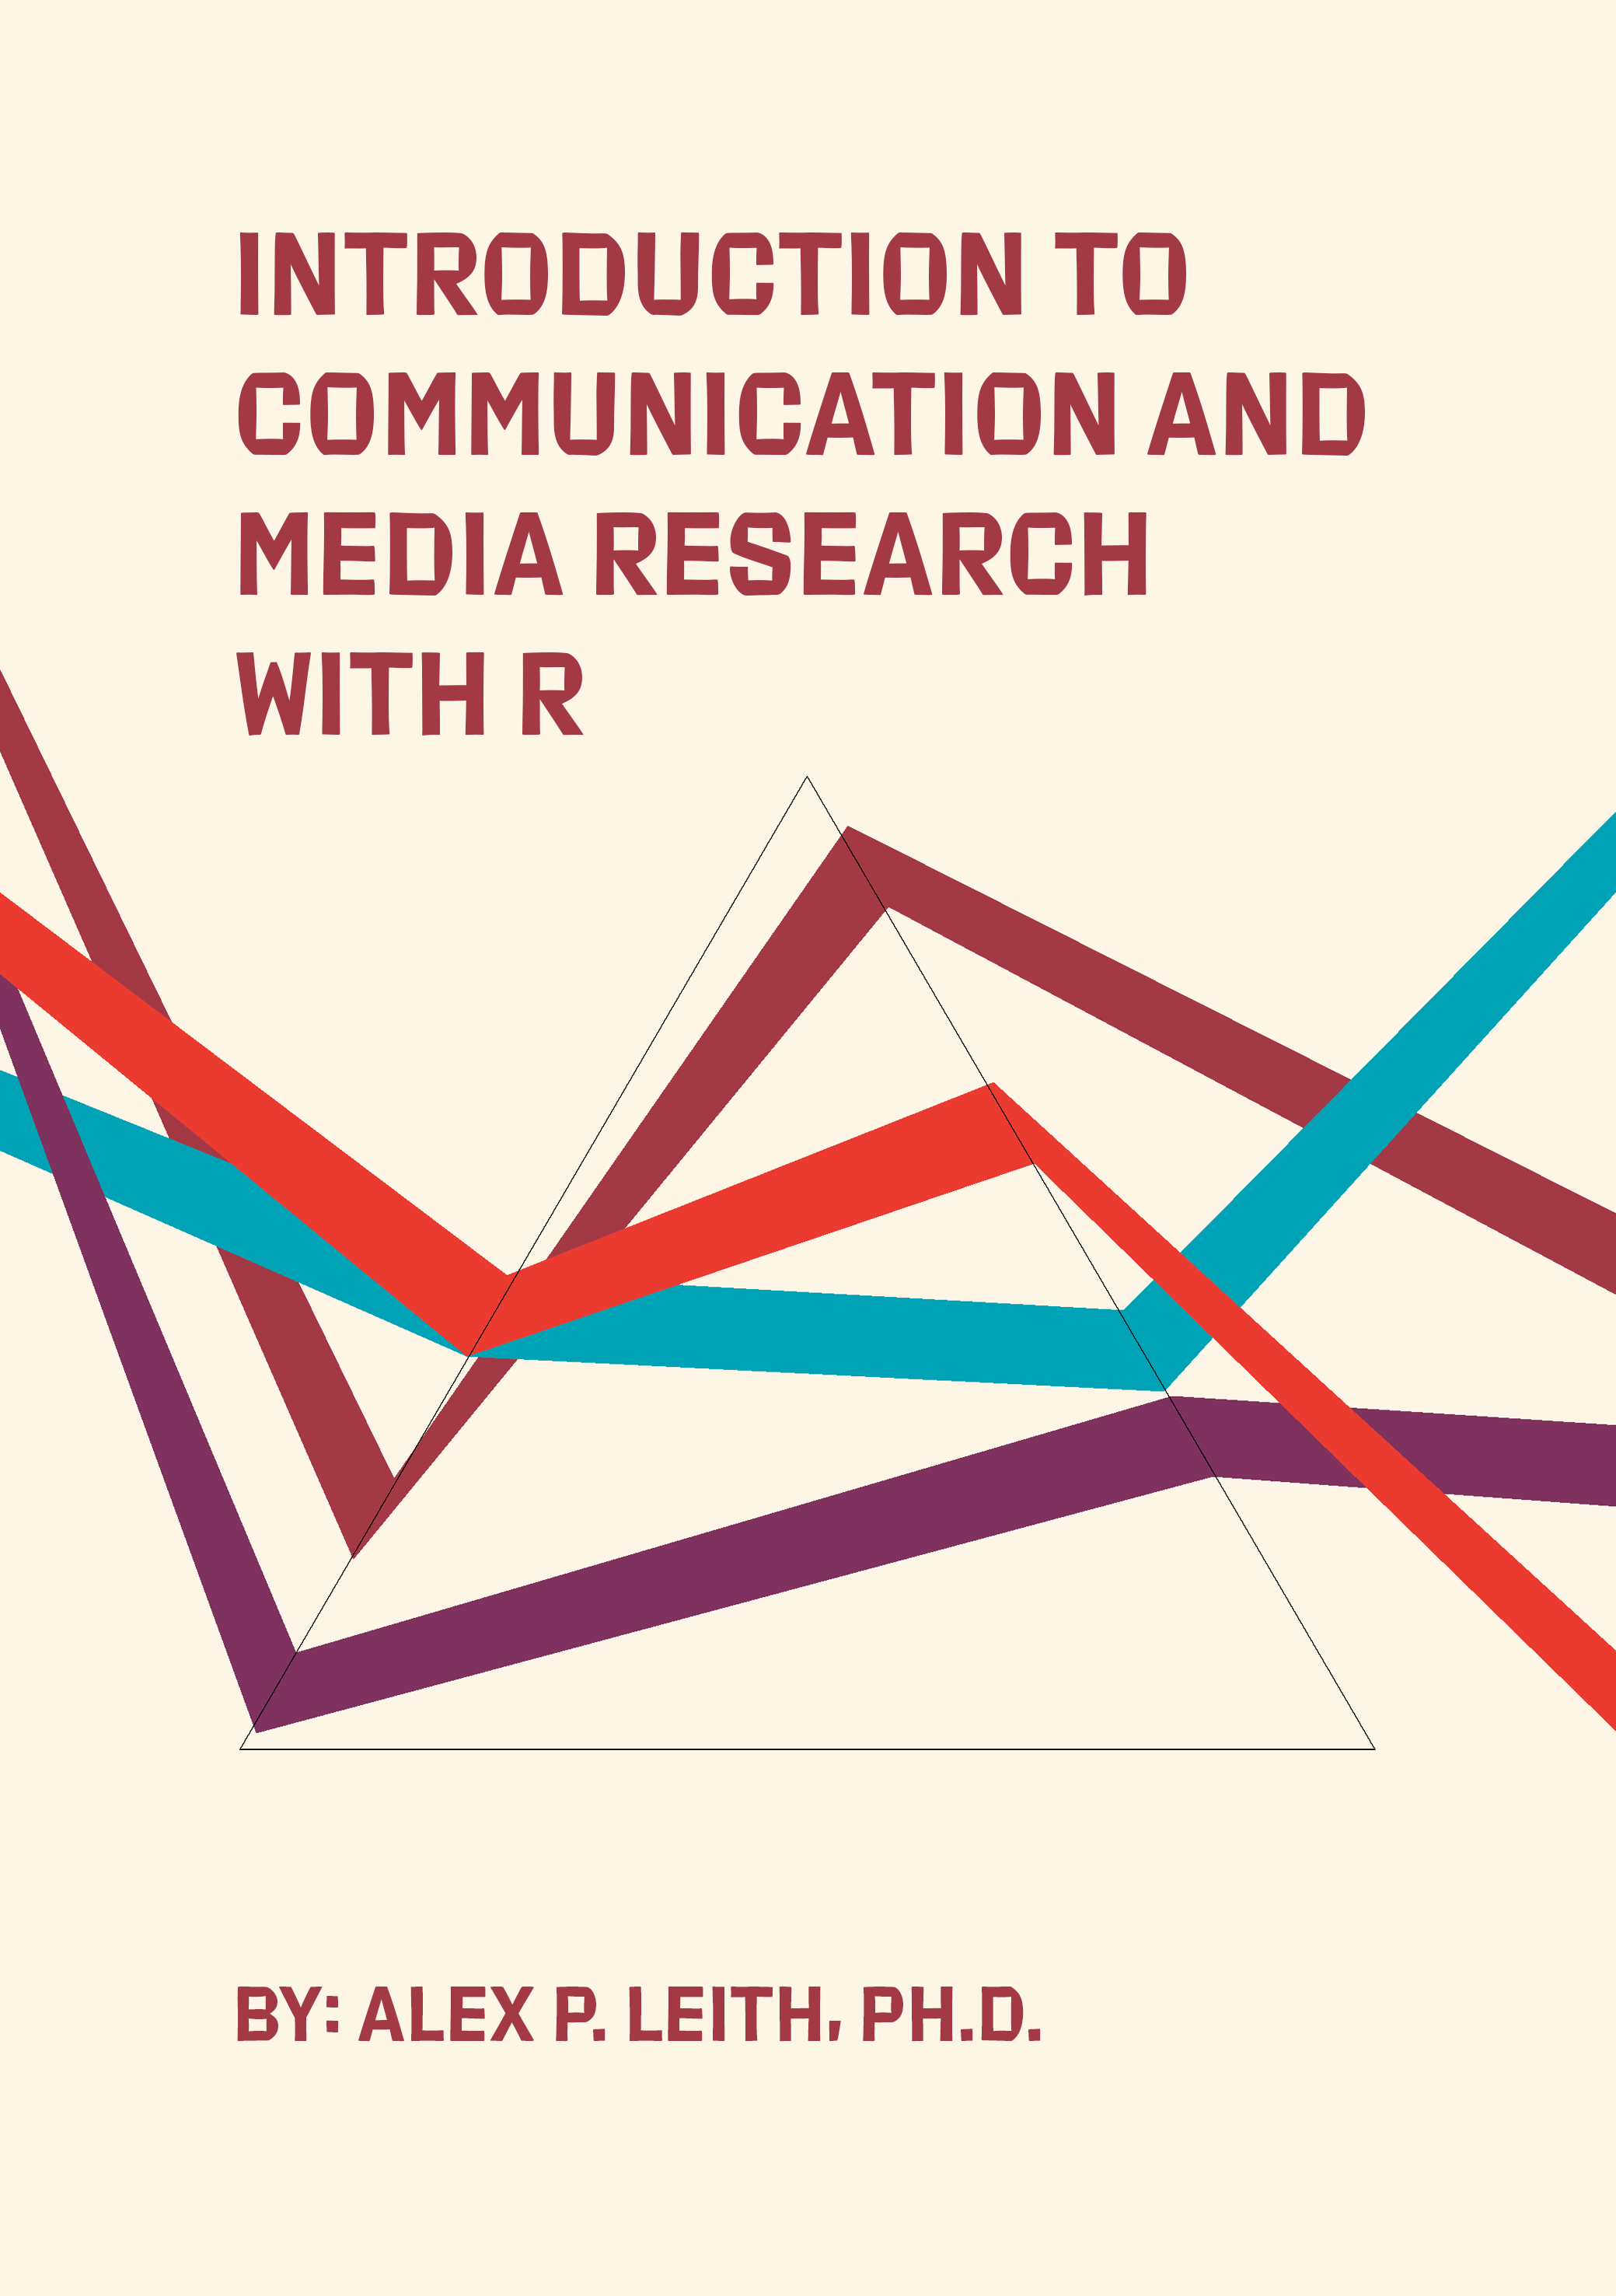
\includegraphics[width=0.5\textwidth,height=\textheight]{cover_2.png}}

This is an open-access textbook primarily created for my MC 451 course at Southern Illinois University Edwardsville (SIUE). I believe that it is important for our media and communication students to learn skills like R to better prepare them for the future of this industry.

Because coding is so frustrating to new learners, I hope this book will demystify the R language enough that they can use it to separate themselves in their future career. I also hope to make them more willing to tackle new complex systems on their own to continue to grow into the future of the communication and media fields.

This is a living document that will be continually adjusted according to feedback from other scholars and students. The current version of this book is a result of multiple semesters of teaching R to students in the Mass Communications department at SIUE, at both the undergraduate and graduate levels.

I would like to thank, and apologize to, each student that has trudged their way through this process with me. Your feedback has been greatly appreciated and instructive. I hope that each semester continues to become more approachable to students.

\hypertarget{introduction}{%
\chapter{Introduction}\label{introduction}}

Welcome to \emph{Introduction to Communication and Media Research with R}. I am Alex P. Leith, an Assistant Professor in the Mass Communications department at Southern Illinois University Edwardsville. While a doctoral student at Michigan State University, I fell in love with the flexibility of the R program for data collection, cleaning, analysis, and visualization. My intention with this book is to build an introductory research book for communication and media professionals that are tasked with research. For college students, this text is intended for individuals with either zero or limited research experience.

This book is also a practice in applying generative pre-trained transformers (GPT) in writing drafts. Namely, the first draft of this paper is a mix of human and AI writing. As I continue to work on this book, I will clean the text until limited traces of AI remain. I am using AI (e.g., Chat GPT, Google Bard) to identify future uses of these tools that still allow for individual work and learning opportunities. This book also borrows structure from existing research methods books. Images are pulled from royalty-free locations, such as Unsplash and Wikimedia.

Communication research systematically studies the processes, antecedents, and consequences of communication. It is a broad field encompassing various topics, from interpersonal to mass communication. Media research is the study of the effects of mass media on society, culture, and individuals. It encompasses a wide range of topics, including the impact of media on news consumption, political attitudes, and consumer behavior. Communication and media researchers use various methods to collect data, including surveys, interviews, focus groups, and experiments.

\hypertarget{research-ethics}{%
\section*{Research Ethics}\label{research-ethics}}

Research ethics is the set of moral principles that guide the conduct of research. It is essential to ensure that research is conducted ethically to protect the rights and welfare of research participants, ensure the validity of research findings, and build public trust in research. Several ethical principles are relevant to research, including respect for persons, beneficence, and justice. In addition to these general ethical principles, there are also specific ethical guidelines for different types of research.

\hypertarget{research-papers}{%
\section*{Research Papers}\label{research-papers}}

An academic research paper is a piece of writing that presents the results of original research on a particular topic. It is typically written in a formal style and follows a specific format. Academic research papers are usually published in academic journals or presented at conferences. Research papers are discoverable through search engines available through academic libraries, publishers' websites, and search engines (e.g., Google Scholar).

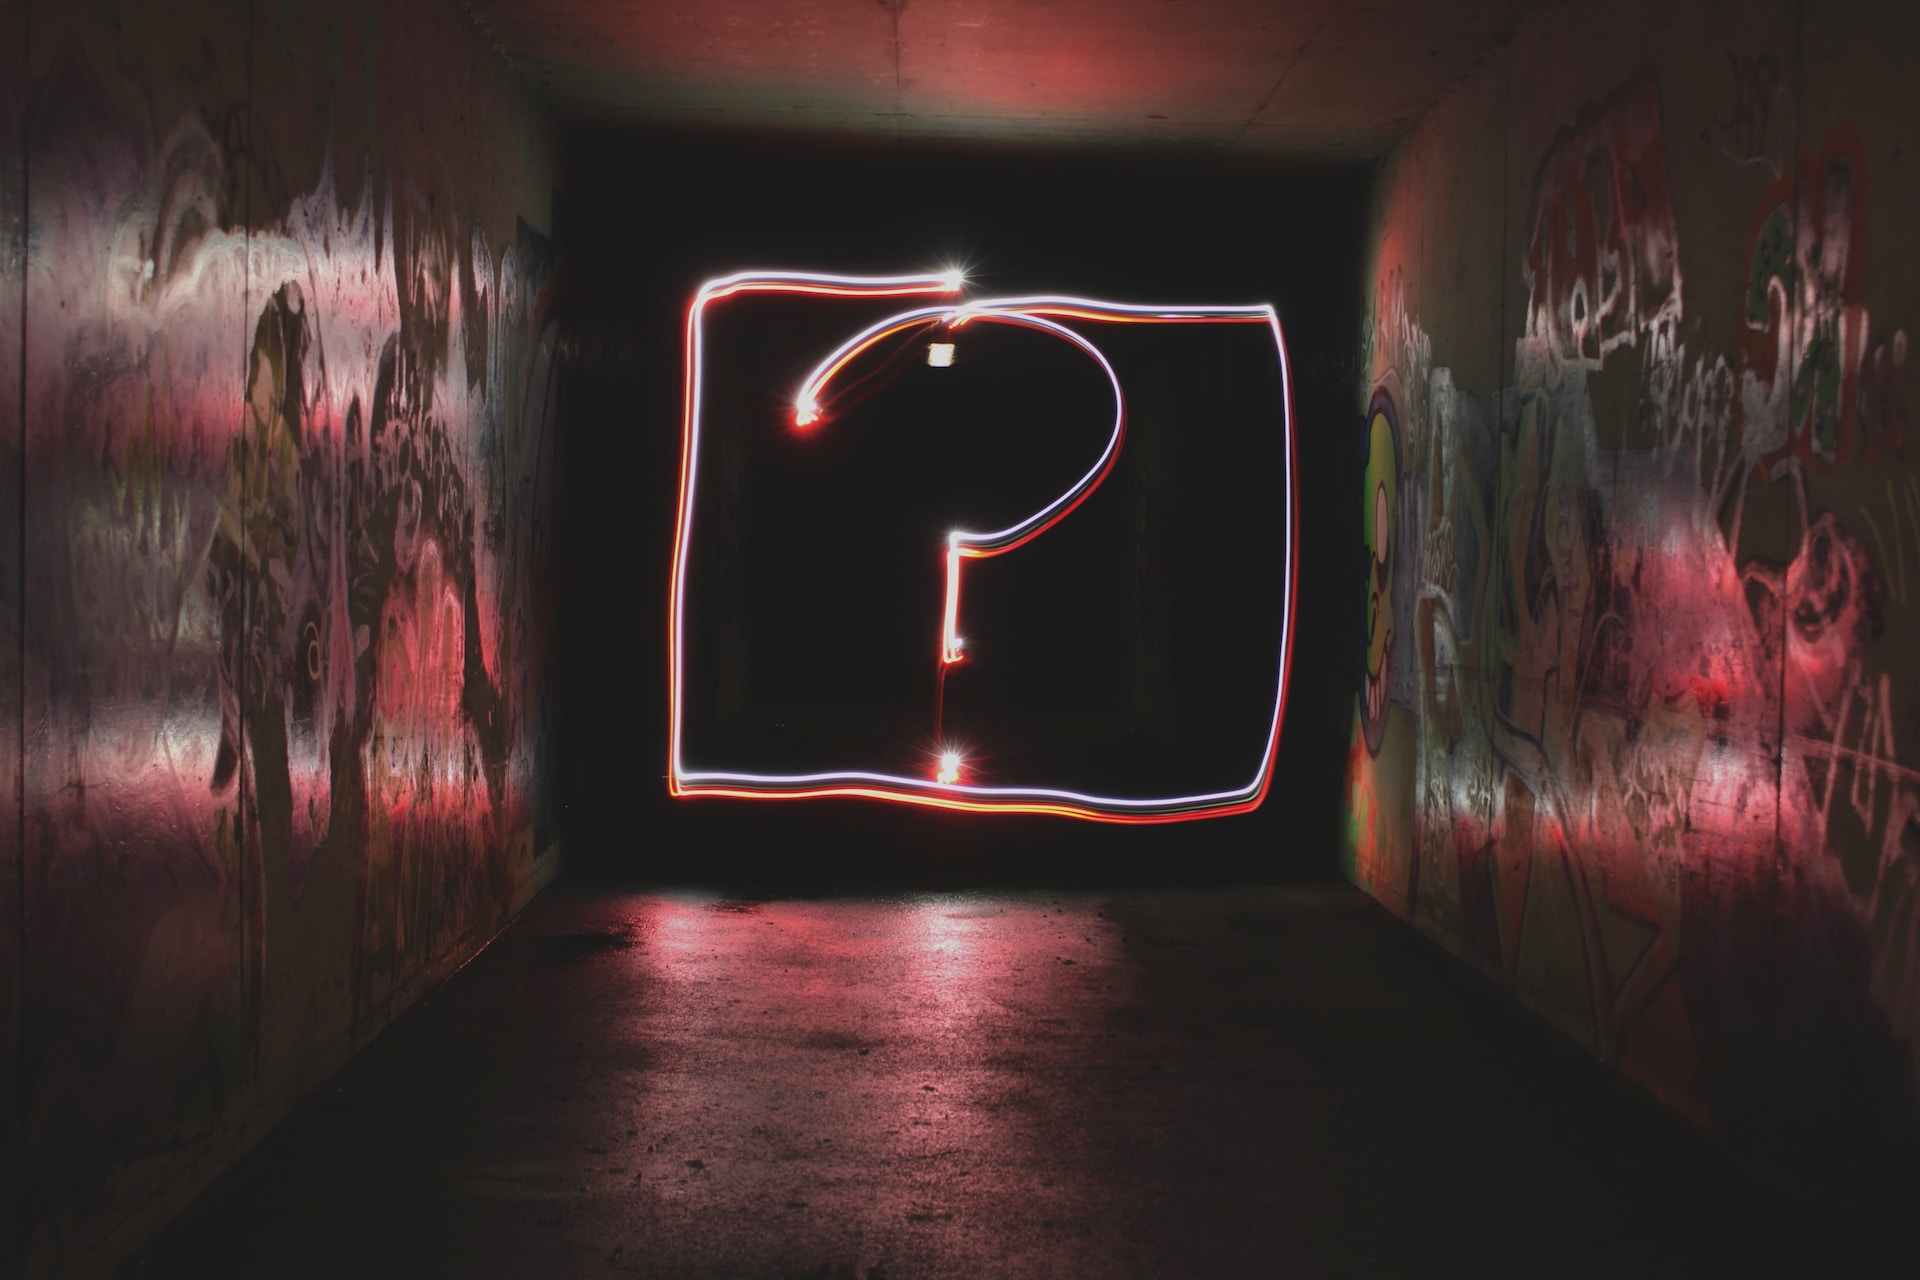
\includegraphics[width=1\textwidth,height=\textheight]{images/question_mark.jpg}

\hypertarget{communication-theories}{%
\section*{Communication Theories}\label{communication-theories}}

Communication and media theories are a set of concepts and frameworks that help us understand how people communicate and how the media influences our lives. These theories can be used to analyze a wide range of communication phenomena, from interpersonal communication to mass media. Each theory offers a different perspective on how communication and the media work. By understanding these theories, we can better understand how people communicate and how the media influences our lives.

\hypertarget{interviews}{%
\section*{Interviews}\label{interviews}}

Interviews are a research method in which the interviewer gathers information from the interviewee through open-ended questions and follow-up questions. The goal of a qualitative interview is to understand the interviewee's experiences, perspectives, and beliefs on a particular topic. Qualitative interviews are often used in social science research, but they can also be used in other fields, such as business, healthcare, and education. They are a valuable tool for gathering in-depth information that cannot be easily obtained through other methods, such as surveys or questionnaires. Interviews can be a valuable tool for researchers who want to understand the experiences, perspectives, and beliefs of people on a particular topic. However, it is important to note that qualitative interviews are not without their challenges. They can be time-consuming and expensive to conduct, and the data can be difficult to analyze. Additionally, the interviewer's own biases can influence the results of the interview.

\hypertarget{focus-groups}{%
\section*{Focus Groups}\label{focus-groups}}

Focus groups are a research method in which a group of people are brought together to discuss a particular topic. The facilitator of the focus group asks open-ended questions and encourages the participants to share their thoughts and experiences. The goal of a focus group is to get a variety of perspectives on a particular topic and to understand how people interact with each other and with the topic. Focus groups can be a valuable tool for researchers who want to understand the perspectives of a group of people on a particular topic. However, it is important to note that qualitative focus groups are not without their challenges. They can be time-consuming and expensive to conduct, and the data can be difficult to analyze. Additionally, the facilitator's own biases can influence the results of the focus group.

\hypertarget{ethnography}{%
\section*{Ethnography}\label{ethnography}}

Ethnography is a research method that involves immersing the researcher in a particular culture or community to study its social interactions, behaviors, and beliefs. The researcher typically conducts participant observation, interviews, and document analysis to gather data. The goal of qualitative ethnography is to gain a deep understanding of the culture or community from the insider's perspective. Ethnography can be a valuable tool for researchers who want to understand the culture or community of a particular group of people. However, it is important to note that qualitative ethnography is not without its challenges. It can be time-consuming and expensive to conduct, and the researcher's own biases can influence the results of the study.

\hypertarget{qualitative-content-analysis}{%
\section*{Qualitative Content Analysis}\label{qualitative-content-analysis}}

Qualitative content analysis is a research method for the subjective interpretation of the content of text data through the systematic classification process of coding and identifying themes or patterns. The goal of qualitative content analysis is to understand the meaning of the text data by identifying patterns and themes. Qualitative content analysis can be a valuable tool for researchers who want to understand the meaning of text data. However, it is important to note that qualitative content analysis is not without its challenges. It can be time-consuming and labor-intensive to conduct, and the researcher's own biases can influence the results of the analysis.

\hypertarget{quantitative-content-analysis}{%
\section*{Quantitative Content Analysis}\label{quantitative-content-analysis}}

Quantitative content analysis is a research method for the objective, systematic, and quantitative description of the content of text data. The goal of quantitative content analysis is to quantify the presence of certain words, phrases, or concepts in a text and to analyze the relationships between these features. Quantitative content analysis can be a valuable tool for researchers who want to quantify the presence of certain words, phrases, or concepts in a text. However, it is important to note that quantitative content analysis is not without its challenges. It can be time-consuming and labor-intensive to conduct, and the researcher's own biases can still influence the results of the analysis.

\hypertarget{surveys}{%
\section*{Surveys}\label{surveys}}

Surveys are a research method in which a researcher asks a set of questions to a group of people in order to collect numerical data. The data is then analyzed to answer research questions or test hypotheses. Surveys can be a valuable tool for researchers who want to collect data about a large group of people. However, it is important to note that quantitative surveys are not without their challenges. They can be time-consuming and expensive to conduct, and the respondents may not always answer the questions honestly or accurately.

\hypertarget{experiment}{%
\section*{Experiment}\label{experiment}}

Experiment are research studies that use a scientific approach to test a hypothesis. The researcher manipulates one or more variables and then measures the effects of the manipulation on one or more other variables. Experiment can be a valuable tool for researchers who want to test a hypothesis and to determine the cause and effect relationship between two or more variables. However, it is important to note that quantitative experiments are not without their challenges. They can be time-consuming and expensive to conduct, and the results can be affected by the way the experiment is conducted.

\hypertarget{introduction-to-r}{%
\section*{Introduction to R}\label{introduction-to-r}}

R is a programming language and software environment for statistical computing and graphics. It is a free and open-source software environment, making it available to everyone to use and modify. R is used by statisticians, data miners, and researchers in various fields. The program allows individuals to use code to expedite data cleaning and analysis tasks. Users are also provided with a range of options for data visualization.

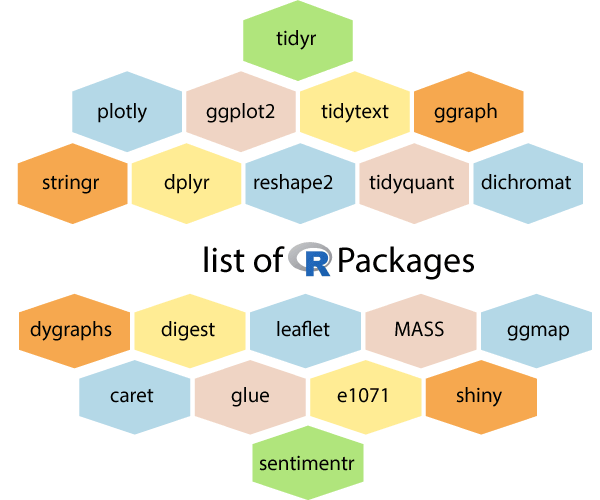
\includegraphics[width=1\textwidth,height=\textheight]{images/List-of-r-packages.png}

\hypertarget{working-with-data}{%
\section*{Working with Data}\label{working-with-data}}

Data is a collection of facts, figures, or observations that can be used to answer questions or test hypotheses. Data can be collected from various sources, including surveys, experiments, and observations. Once data has been collected, it needs to be prepared for analysis. This process typically involves cleaning the data, formatting the data, and transforming the data. Researchers can either use R for these stages or external programs (e.g., Excel).

\hypertarget{visuals}{%
\section*{Visuals}\label{visuals}}

There are many different types of data visualization, each with strengths and weaknesses. Some of the most common types of data visualization include bar charts, scatter plots, images, or tables. The best kind of data visualization for a particular dataset depends on the specific research question and the study's goals. Choosing a data visualization that is easy to understand and accurately represents the data is essential.

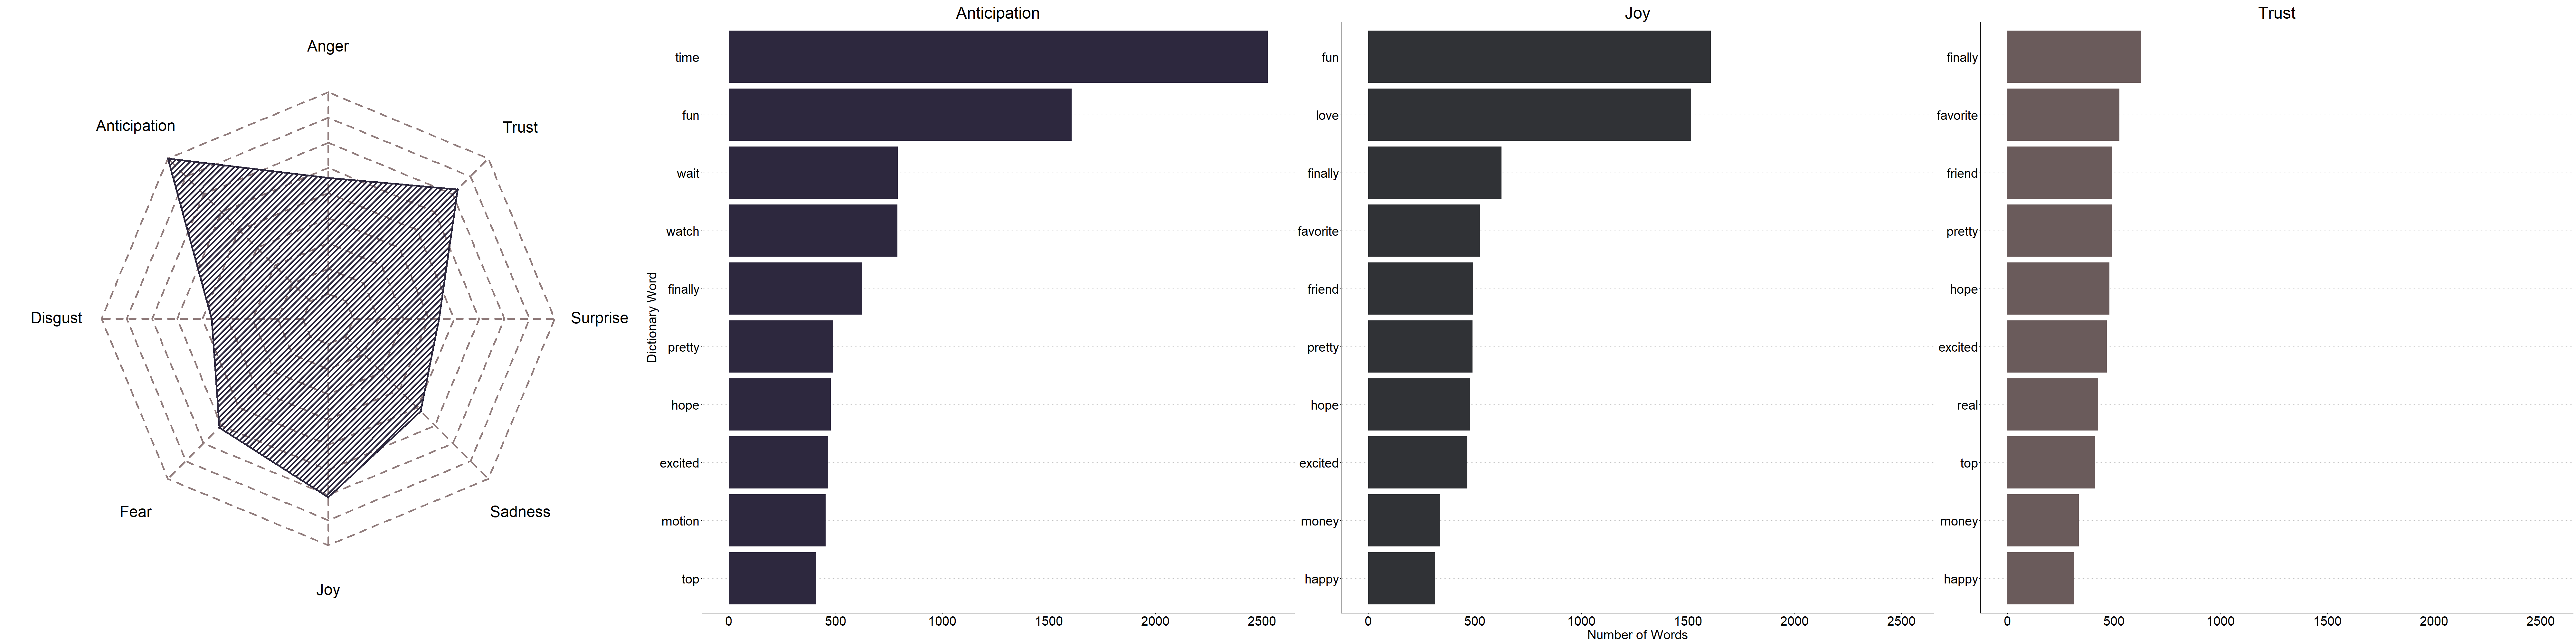
\includegraphics[width=1\textwidth,height=\textheight]{images/VR-Play-Emotion-MP.png}

\hypertarget{analyses}{%
\section*{Analyses}\label{analyses}}

Data analysis is the process of inspecting, cleaning, transforming, and modeling data to discover useful information, inform conclusions, and support decision-making. Data analysis has multiple facets and approaches, encompassing diverse techniques under various names in different business, science, and social science domains. For our context, we are most interested in descriptive and inferential statistics. Descriptive statistics are used to summarize data and describe its main features. They can be used to calculate measures of central tendency (such as the mean, median, and mode) and measures of variation (such as the standard deviation). Inferential statistics are used to make inferences about a population based on a sample. They can be used to test hypotheses and estimate parameters. The best type of data analysis for a particular dataset will depend on the specific research question being asked and the goals of the study. Choosing a data analysis method that is appropriate for the data and will help answer the research question is vital.

\hypertarget{research-ethics-1}{%
\chapter{Research Ethics}\label{research-ethics-1}}

\hypertarget{history}{%
\section{History}\label{history}}

The history of research ethics in social science is a long and complex one. It has been shaped by a number of factors, including the development of new research methods, the rise of social movements, and public awareness of ethical violations.

In the early days of social science research, there were few formal ethical guidelines. Researchers often conducted their studies without any regard for the rights or welfare of their participants. This led to a number of high-profile ethical violations, such as the Tuskegee Syphilis Study and the Milgram Experiments.

These ethical violations led to a growing awareness of the need for ethical standards in social science research. In 1974, the U.S. Congress passed the National Research Act, which established the National Commission for the Protection of Human Subjects of Biomedical and Behavioral Research. This commission was tasked with developing ethical guidelines for social science research.

The commission's report, ``The Belmont Report,'' outlined three basic ethical principles for social science research: respect for persons, beneficence, and justice. These principles have been widely adopted by social scientists and have helped to shape the ethical landscape of social science research.

In recent years, there has been a growing emphasis on the need for cultural sensitivity in social science research. This is due in part to the increasing diversity of the world's population and the growing awareness of the ways in which culture can shape research findings.

As a result of these developments, the field of research ethics in social science is constantly evolving. New ethical challenges are emerging all the time, and researchers must be prepared to adapt their practices accordingly.

\hypertarget{key-events}{%
\subsection*{Key Events}\label{key-events}}
\addcontentsline{toc}{subsection}{Key Events}

\begin{itemize}
\tightlist
\item
  1949: The Nuremberg Code is adopted, outlining ethical principles for medical research involving human subjects.
\item
  1964: The Declaration of Helsinki is adopted, providing recommendations for biomedical research involving human subjects.
\item
  1974: The National Research Act is passed, establishing the National Commission for the Protection of Human Subjects of Biomedical and Behavioral Research.
\item
  1979: The Belmont Report is published, outlining three basic ethical principles for social science research: respect for persons, beneficence, and justice.
\item
  1991: The American Psychological Association adopts its first code of ethics for research with human participants.
\item
  2002: The National Bioethics Advisory Commission issues its report, ``Ethical and Policy Issues in Human Stem Cell Research,'' which discusses the ethical implications of stem cell research.
\item
  2013: The American Sociological Association adopts its first code of ethics for research with human participants.
\end{itemize}

\hypertarget{unethical-research}{%
\subsection*{Unethical Research}\label{unethical-research}}
\addcontentsline{toc}{subsection}{Unethical Research}

\hypertarget{the-tuskegee-syphilis-study}{%
\subsubsection*{The Tuskegee Syphilis Study}\label{the-tuskegee-syphilis-study}}
\addcontentsline{toc}{subsubsection}{The Tuskegee Syphilis Study}

This study, which ran from 1932 to 1972, involved 600 African American men who were infected with syphilis but not treated. The researchers observed the men's progression of the disease without providing them with treatment, even after penicillin became available. This study was unethical because it violated the men's right to informed consent and because it exposed them to unnecessary harm.

\hypertarget{the-milgram-experiments}{%
\subsubsection*{The Milgram Experiments}\label{the-milgram-experiments}}
\addcontentsline{toc}{subsubsection}{The Milgram Experiments}

These experiments, which were conducted by Stanley Milgram in the 1960s, investigated obedience to authority. In the experiments, participants were told to deliver electric shocks to another person, who was actually an actor. The shocks were fake, but the participants did not know this. Many of the participants continued to deliver shocks even when the actor was begging them to stop. This study was unethical because it caused psychological distress to the participants.

\hypertarget{the-milgram-experimentsthe-stanford-prison-experiment}{%
\subsubsection*{\texorpdfstring{\protect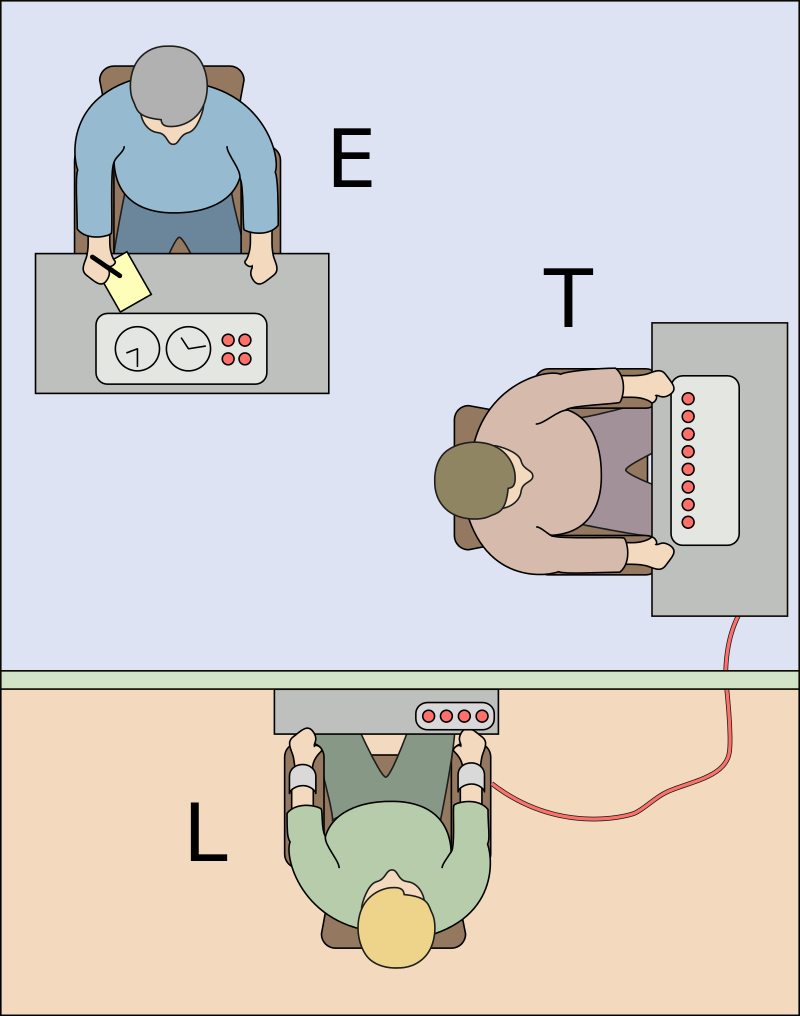
\includegraphics[width=0.45\textwidth,height=\textheight]{images/Milgram_experiment.png}\protect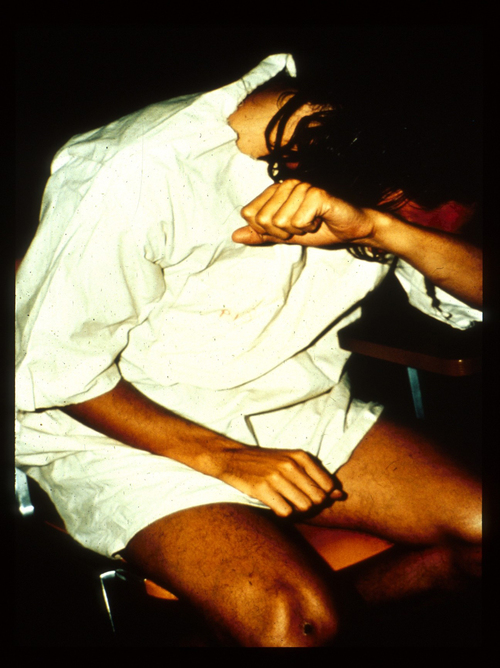
\includegraphics[width=0.45\textwidth,height=\textheight]{images/prisoner-breaks-down.png}}{The Milgram ExperimentsThe Stanford Prison Experiment}}\label{the-milgram-experimentsthe-stanford-prison-experiment}}
\addcontentsline{toc}{subsubsection}{}

\hypertarget{the-stanford-prison-experiment}{%
\subsubsection*{The Stanford Prison Experiment}\label{the-stanford-prison-experiment}}
\addcontentsline{toc}{subsubsection}{The Stanford Prison Experiment}

This experiment, which was conducted by Philip Zimbardo in 1971, simulated a prison environment. Participants were randomly assigned to be either guards or prisoners. The guards quickly began to abuse the prisoners, and the prisoners became increasingly submissive. This study was unethical because it created a stressful and potentially harmful environment for the participants. These are just a few examples of unethical applications of social science research. These studies have helped to raise awareness of the importance of ethical research practices, and they have led to the development of ethical guidelines for social science research.

\hypertarget{key-components}{%
\section{Key Components}\label{key-components}}

There are several key components of ethical research. These include informed consent, confidentiality, debriefing, avoidance of harm, and justice. Each must be present for ethical research.

\hypertarget{informed-consent}{%
\subsection*{Informed Consent}\label{informed-consent}}
\addcontentsline{toc}{subsection}{Informed Consent}

Participants must be given adequate information about the research in order to make an informed decision about whether or not to participate. This information should include title of project, names of researchers, contact info for researchers, purpose of study, procedures, risks \& benefits, and anonymity, voluntary participation.

\hypertarget{confidentiality}{%
\subsection*{Confidentiality}\label{confidentiality}}
\addcontentsline{toc}{subsection}{Confidentiality}

The privacy of participants must be protected. This means that researchers must not share personal information about participants without their consent.

\hypertarget{debriefing}{%
\subsection*{Debriefing}\label{debriefing}}
\addcontentsline{toc}{subsection}{Debriefing}

Participants must be debriefed after the research is completed. This means that they must be given more information about the research, including any deception that was used. Participants also have the right to ask questions and to have their concerns addressed.

\hypertarget{avoidance-of-harm}{%
\subsection*{Avoidance of Harm}\label{avoidance-of-harm}}
\addcontentsline{toc}{subsection}{Avoidance of Harm}

Participants must not be harmed by the research. This means that researchers must take steps to minimize the risks of harm to participants.

\hypertarget{justice}{%
\subsection*{Justice}\label{justice}}
\addcontentsline{toc}{subsection}{Justice}

The benefits and burdens of research must be distributed fairly. This means that researchers must ensure that all participants have an equal opportunity to benefit from the research, and that no one group is disproportionately burdened by the research.

\hypertarget{ethical-considerations}{%
\section{Ethical Considerations}\label{ethical-considerations}}

In addition to these key components, there are a number of other ethical considerations that researchers must take into account. Researchers must carefully consider all of these ethical issues when designing and conducting research. By following ethical principles, researchers can help to ensure that their research is conducted in an ethical manner and that the rights and welfare of participants are protected.

\hypertarget{deception}{%
\subsection*{Deception}\label{deception}}
\addcontentsline{toc}{subsection}{Deception}

Deception can be used in research to prevent participants from guessing the purpose of the study. However, deception can also harm participants by making them feel misled or violated.

\hypertarget{risks-to-participants}{%
\subsection*{Risks to Participants}\label{risks-to-participants}}
\addcontentsline{toc}{subsection}{Risks to Participants}

Some research involves risks to participants, such as physical or psychological harm. These risks must be weighed against the potential benefits of the research before participants can consent to participate.

\hypertarget{vulnerable-populations}{%
\subsection*{Vulnerable Populations}\label{vulnerable-populations}}
\addcontentsline{toc}{subsection}{Vulnerable Populations}

Some populations are more vulnerable to harm from research, such as children, prisoners, and people with disabilities. These populations require special protections in research.

\hypertarget{intellectual-property}{%
\subsection*{Intellectual Property}\label{intellectual-property}}
\addcontentsline{toc}{subsection}{Intellectual Property}

Researchers must be careful not to violate the intellectual property rights of others, such as by publishing data without permission or using copyrighted materials without permission.

\hypertarget{current-ethical-challenges-in-social-science-research}{%
\section{Current Ethical Challenges in Social Science Research}\label{current-ethical-challenges-in-social-science-research}}

The use of new technologies, such as social media and big data, raises new ethical challenges. The need for cultural sensitivity in social science research is becoming increasingly important. The tension between the need for confidentiality and the need to share research findings with the public is a challenge that researchers must grapple with. The increasing commercialization of social science research raises ethical concerns about the potential for conflicts of interest.

\hypertarget{institutional-review-board}{%
\section{Institutional Review Board}\label{institutional-review-board}}

\hypertarget{history-of-the-institutional-review-board}{%
\subsection*{History of the Institutional Review Board}\label{history-of-the-institutional-review-board}}
\addcontentsline{toc}{subsection}{History of the Institutional Review Board}

The Institutional Review Board (IRB) is a committee that reviews research involving human subjects to ensure that the research is conducted ethically. IRBs are required by law in the United States and in many other countries.

The history of IRBs can be traced back to the Nuremberg Code, which was adopted in 1949 in response to the atrocities committed by Nazi doctors during World War II. The Nuremberg Code established basic ethical principles for medical research involving human subjects, including the need for informed consent and the avoidance of unnecessary harm.

In 1964, the Declaration of Helsinki was adopted, providing additional guidance on ethical research practices. The Declaration of Helsinki was revised in 2013 to reflect the changing landscape of biomedical research.

In the United States, the National Research Act of 1974 established the National Commission for the Protection of Human Subjects of Biomedical and Behavioral Research. The commission was tasked with developing ethical guidelines for research involving human subjects. The commission's report, ``The Belmont Report,'' outlined three basic ethical principles for research involving human subjects: respect for persons, beneficence, and justice.

The Belmont Report has been widely adopted by IRBs and has helped to shape the ethical landscape of research involving human subjects. IRBs are responsible for ensuring that research involving human subjects is conducted in accordance with the ethical principles outlined in the Belmont Report.

\hypertarget{purpose-of-the-institutional-review-board}{%
\subsection*{Purpose of the Institutional Review Board}\label{purpose-of-the-institutional-review-board}}
\addcontentsline{toc}{subsection}{Purpose of the Institutional Review Board}

The purpose of the IRB is to protect the rights and welfare of human subjects involved in research. IRBs do this by reviewing research proposals to ensure that they meet ethical standards. IRBs play an important role in protecting the rights and welfare of human subjects involved in research. By reviewing research proposals and ensuring that research is conducted in accordance with ethical standards, IRBs help to ensure that research is conducted in a responsible and ethical manner.

IRBs review research proposals for a number of factors, including:

\begin{itemize}
\tightlist
\item
  The risks and benefits of the research
\item
  The informed consent process
\item
  The protection of confidentiality
\item
  The selection of research subjects
\end{itemize}

If an IRB finds that a research proposal does not meet ethical standards, the proposal may be modified or rejected.

\hypertarget{levels-of-risk}{%
\subsection*{Levels of Risk}\label{levels-of-risk}}
\addcontentsline{toc}{subsection}{Levels of Risk}

The three levels of risk for IRB are:

\hypertarget{exempt}{%
\subsubsection*{Exempt}\label{exempt}}
\addcontentsline{toc}{subsubsection}{Exempt}

Studies that meet the criteria for exemption from IRB review do not pose more than minimal risk to participants. Examples of exempt studies include:

\begin{itemize}
\item
  Research using existing data or records that cannot be linked back to individual participants.
\item
  Research involving surveys or interviews that do not ask about sensitive topics.
\item
  Research involving the observation of public behavior.
\end{itemize}

\hypertarget{expedited}{%
\subsubsection*{Expedited}\label{expedited}}
\addcontentsline{toc}{subsubsection}{Expedited}

Studies that involve no more than minimal risk to participants and meet the criteria for expedited review may be reviewed by a single IRB reviewer or a small committee of reviewers. Examples of expedited studies include:

\begin{itemize}
\item
  Research involving the use of noninvasive procedures, such as blood pressure checks or physical exams.
\item
  Research involving the collection of non-sensitive data, such as demographic information or data about food choices.
\item
  Research involving the use of existing data or records that can be linked back to individual participants, but only if the data is de-identified.
\end{itemize}

\hypertarget{full}{%
\subsubsection*{Full}\label{full}}
\addcontentsline{toc}{subsubsection}{Full}

Studies that involve more than minimal risk to participants or do not meet the criteria for exempt or expedited review must be reviewed by the full IRB. Examples of full board studies include:

\begin{itemize}
\item
  Research involving the use of invasive procedures, such as surgery or blood draws.
\item
  Research involving the collection of sensitive data, such as information about mental health or sexual behavior.
\item
  Research involving the use of deception or coercion.
\end{itemize}

\hypertarget{references}{%
\section{References}\label{references}}

American Psychological Association (2017). Ethical principles of psychologists and code of conduct. Retrieved from \url{https://www.apa.org/ethics/code/}

Brandt, A. M. (1978). Racism and research: The case of the Tuskegee Syphilis Study. Daedalus, 107(2), 17-41.

Milgram, S. (1974). Obedience to authority: An experimental view. New York, NY: Harper \& Row.

National Commission for the Protection of Human Subjects of Biomedical and Behavioral Research. (1979). The Belmont Report: Ethical principles and guidelines for the protection of human subjects of research. Washington, DC: U.S. Government Printing Office.

National Institutes of Health (2019). Protecting human subjects. Retrieved from \url{https://humansubjects.nih.gov/}

Office for Human Research Protections (2022). Protecting human subjects. Retrieved from \url{https://www.hhs.gov/ohrp/index.html}

U.S. Department of Health and Human Services. (2018). Protection of human subjects. Retrieved from \url{https://www.hhs.gov/ohrp/humansubjects/index.html}

Zimbardo, P. G. (2007). The Lucifer effect: Understanding how good people turn evil. New York, NY: Random House.

\hypertarget{research-papers-1}{%
\chapter{Research Papers}\label{research-papers-1}}

\hypertarget{find}{%
\section{How to Find Research Papers}\label{find}}

There are many ways to find research papers, both paid and free. Here are a few popular methods:

\hypertarget{use-a-specialized-search-engine.}{%
\subsection*{Use a specialized search engine.}\label{use-a-specialized-search-engine.}}
\addcontentsline{toc}{subsection}{Use a specialized search engine.}

Specialized search engines are designed to search for specific types of information, such as research articles. Here are some tips on how to use a specialized search engine to find research articles:

\textbf{Choose the right search engine.} There are many specialized search engines available, so it is important to choose one that is relevant to your topic. Some popular specialized search engines for research articles include:

\begin{itemize}
\item
  Google Scholar
\item
  PubMed
\item
  Web of Science
\item
  Scopus
\item
  IEEE Xplore
\item
  ACM Digital Library
\end{itemize}

\textbf{Use keywords.} When you are searching for research articles, it is important to use keywords that are relevant to your topic. You can use the same keywords that you would use for a general search engine, but you may also need to use more specific keywords.

\textbf{Use advanced search features.} Most specialized search engines have advanced search features that allow you to narrow down your search results. For example, you can specify the publication date, the language, or the type of document.

\textbf{Read the results carefully.} Once you have found some research articles, take some time to read them carefully. This will help you identify the articles that are most relevant to your research.

\textbf{Evaluate the quality of the sources.} Not all sources are created equal. When you are evaluating the quality of a research article, consider the following factors:

\begin{itemize}
\item
  The author's credentials
\item
  The publication date
\item
  The journal's reputation
\item
  The methodology used
\item
  The findings of the study
\end{itemize}

By following these tips, you can use a specialized search engine to find research articles that are relevant to your topic and of high quality.

Here are some additional tips for using a specialized search engine to find research articles:

\textbf{Use quotation marks to search for exact phrases.} For example, if you are looking for articles about the ``impact of social media on mental health,'' you would search for ``impact of social media on mental health.''

\textbf{Use Boolean operators to combine keywords.} Boolean operators, such as AND, OR, and NOT, can be used to combine keywords and narrow down your search results. For example, if you are looking for articles about the ``impact of social media on mental health'' in the journal ``Nature,'' you would search for ``impact of social media AND mental health AND Nature.''

\textbf{Use filters to narrow down your results.} Most specialized search engines allow you to filter your results by publication date, language, and other criteria. This can be helpful if you are looking for specific types of research articles.

\textbf{Use the search engine's help documentation.} Most specialized search engines have help documentation that can provide you with more information about how to use the search engine.

I hope these tips help you find the research articles you are looking for.

\hypertarget{check-your-university-library.}{%
\subsection*{Check your university library.}\label{check-your-university-library.}}
\addcontentsline{toc}{subsection}{Check your university library.}

Your university library has a wealth of resources that you can use to find research articles. Here are some tips on how to use your university library to find research articles:

\textbf{Talk to a librarian.} Librarians are experts in finding information. They can help you choose the right databases and search strategies for your research.

\textbf{Use the library's online catalog.} The library's online catalog is a searchable database of all the books, journals, and other materials that the library owns.

\textbf{Use the library's databases.} The library subscribes to a variety of databases that contain research articles. These databases can be searched by keyword, author, or subject.

\textbf{Ask for help from a research assistant.} Many libraries have research assistants who can help you find research articles.

\hypertarget{search-for-preprints.}{%
\subsection*{Search for preprints.}\label{search-for-preprints.}}
\addcontentsline{toc}{subsection}{Search for preprints.}

A research preprint is a preliminary version of a research paper that is made available online before it has been peer-reviewed and published in a journal. Preprints are often used by researchers to share their work with the wider community and to get feedback on their findings.

Preprints can be a valuable resource for researchers, as they can provide access to the latest research findings before they are published. They can also help researchers to get feedback on their work and to collaborate with other researchers.

However, it is important to keep in mind that preprints have not been peer-reviewed and may contain errors. Therefore, it is important to evaluate the quality of the preprint carefully before citing it in your own research.

Here are some of the advantages of using preprints:

\textbf{Faster dissemination of research findings.} Preprints can be made available online much faster than traditional journal articles, which can take months or even years to publish. This allows researchers to share their work with the wider community more quickly and to get feedback on their findings.

\textbf{Increased collaboration.} Preprints can be a valuable tool for collaboration, as they allow researchers to share their work with other researchers before it has been published. This can help to identify potential errors and to improve the quality of the research.

\textbf{Reduced publication bias.} Preprints can help to reduce publication bias, which is the tendency for journals to publish research that supports the authors' hypothesis. This is because preprints are not subject to the same peer-review process as journal articles, and therefore, they are more likely to be published regardless of the findings.

Here are some of the disadvantages of using preprints:

\textbf{Unreviewed research.} Preprints have not been peer-reviewed, which means that they may contain errors. Therefore, it is important to evaluate the quality of the preprint carefully before citing it in your own research.

\textbf{Potential for plagiarism.} Preprints are publicly available, which means that there is a potential for plagiarism. Therefore, it is important to give credit to the original authors of the research when you cite a preprint.

\textbf{Legal issues.} There are a number of legal issues that can arise with the use of preprints. For example, it is important to make sure that you have the right to share the preprint and that you are not violating the authors' copyright.

\textbf{Search preprint repositories.} There are a number of preprint repositories that you can search, such as:

\begin{itemize}
\item
  arXiv
\item
  bioRxiv
\item
  medRxiv
\item
  PeerJ Preprints
\item
  PsyArXiv
\item
  SocArXiv
\end{itemize}

\textbf{Use specialized search engines.} There are also a number of specialized search engines that can be used to find preprints, such as:

\begin{itemize}
\item
  Preprints.org
\item
  ASAPbio
\item
  PreLights
\item
  Publons
\end{itemize}

When using preprints, it is important to keep in mind that they have not been peer-reviewed and may contain errors. Therefore, it is important to evaluate the quality of the preprint carefully before citing it in your own research.

Here are some things to consider when evaluating a preprint:

\begin{itemize}
\item
  The author's credentials
\item
  The methodology used
\item
  The findings of the study
\item
  The potential for bias
\end{itemize}

\hypertarget{use-social-media.}{%
\subsection*{Use social media.}\label{use-social-media.}}
\addcontentsline{toc}{subsection}{Use social media.}

You can use social media to find research articles in a few different ways:

\textbf{Follow researchers and research institutions.} Many researchers and research institutions use social media to share their work, including research articles. By following these accounts, you can stay up-to-date on the latest research in your field.

\textbf{Use relevant hashtags.} Hashtags are a great way to find research articles on social media. When you search for a relevant hashtag, you will see all the posts that have been tagged with that hashtag. This can be a great way to find research articles that you might not have otherwise found.

\textbf{Join research groups and communities.} There are many research groups and communities on social media where researchers can share their work and discuss research topics. By joining these groups, you can connect with other researchers and find research articles that are relevant to your interests.

\textbf{Attend online conferences and workshops.} Many conferences and workshops are now being held online, and these can be a great way to find research articles. Often, the presentations from these events are posted online, and you can also interact with the speakers and other attendees.

Here are some specific social media platforms that you can use to find research articles:

\textbf{Twitter:} Twitter is a great platform for following researchers and research institutions. You can also use Twitter to search for research articles using hashtags.

\textbf{LinkedIn:} LinkedIn is a professional networking platform that can be a great way to connect with researchers and find research articles.

\textbf{ResearchGate:} ResearchGate is a social networking platform for researchers. You can use ResearchGate to find research articles, collaborate with other researchers, and get feedback on your own work.

\textbf{Academia.edu:} Academia.edu is a social networking platform for academics. You can use Academia.edu to find research articles, connect with other academics, and share your own work.

\textbf{Facebook:} Facebook can also be a good platform for finding research articles, especially if you are part of a research group or community.

When using social media to find research articles, it is important to be critical of the sources you find. Not all research articles that are shared on social media are of high quality. It is important to evaluate the quality of the article before you cite it in your own research. If you are unsure about the quality of a research article, it is always best to consult with a librarian or another expert.

\hypertarget{contact-experts-in-your-field.}{%
\subsection*{Contact experts in your field.}\label{contact-experts-in-your-field.}}
\addcontentsline{toc}{subsection}{Contact experts in your field.}

There are a few ways to use experts in your field to find research articles:

\textbf{Talk to your professors or advisors.} Your professors and advisors are likely to be familiar with the latest research in your field. They can recommend research articles that you should read and can also help you to identify experts in your field.

\textbf{Attend conferences and workshops.} Attending conferences and workshops is a great way to meet experts in your field and to learn about the latest research. You can also ask experts for recommendations for research articles.

\textbf{Read research blogs and newsletters.} There are many research blogs and newsletters that are written by experts in various fields. These can be a great way to stay up-to-date on the latest research and to find research articles that are relevant to your interests.

\textbf{Use social media.} As mentioned earlier, you can use social media to connect with experts in your field and to find research articles. You can follow researchers and research institutions on Twitter, LinkedIn, and other social media platforms. You can also join research groups and communities on social media.

Here are some specific things you can do to find experts in your field:

\textbf{Search for experts by name or by topic.} There are many online directories that list experts in various fields. You can search for experts by name or by topic.

\textbf{Look for experts who have published research articles in your field.} You can use a specialized search engine, such as Google Scholar, to find research articles that have been published in your field. The authors of these articles are likely to be experts in your field.

\textbf{Look for experts who have given presentations at conferences or workshops in your field.} You can find information about conferences and workshops on the websites of professional organizations.

\textbf{Look for experts who are active on social media.} As mentioned earlier, you can use social media to connect with experts in your field. You can follow researchers and research institutions on Twitter, LinkedIn, and other social media platforms. You can also join research groups and communities on social media.

When using experts in your field to find research articles, it is important to be respectful of their time. When you reach out to an expert, be sure to explain why you are interested in their research and what you are looking for. Be sure to also thank the expert for their time and consideration.

\hypertarget{read}{%
\section{How to Read Research Papers}\label{read}}

There are many different approaches to reading a research paper, but these are some of the most effective ones.

\hypertarget{the-three-pass-approach.}{%
\subsection*{The three-pass approach.}\label{the-three-pass-approach.}}
\addcontentsline{toc}{subsection}{The three-pass approach.}

The three-pass approach to reading a research paper is a method of reading a paper in three stages, each with a specific goal.

\textbf{The first pass}. This is a quick scan to capture a high-level view of the paper. You should read the title, abstract, and introduction carefully, and then skim the rest of the paper, paying attention to the headings and subheadings. The goal of this pass is to get a general understanding of what the paper is about, its main points, and its contributions to the field.

\textbf{The second pass}: This is a more detailed reading of the paper. You should read the introduction and conclusion carefully, and then read the rest of the paper in more detail, paying attention to the methods, results, and discussion. The goal of this pass is to understand the paper's arguments and evidence, and to assess its strengths and weaknesses.

\textbf{The third pass}: This is a critical reading of the paper. You should read the paper carefully, taking notes and challenging the author's assumptions and conclusions. The goal of this pass is to fully understand the paper and to be able to critically evaluate its claims.

\hypertarget{the-question-based-approach.}{%
\subsection*{The question-based approach.}\label{the-question-based-approach.}}
\addcontentsline{toc}{subsection}{The question-based approach.}

The question-based approach to reading a research paper is a method of reading a paper by asking questions about the paper as you read. This approach can help you to focus your reading and to ensure that you understand the key points of the paper.

Here are some questions that you can ask yourself as you read a research paper:

\begin{itemize}
\item
  What is the purpose of the paper?
\item
  What are the main questions that the paper addresses?
\item
  What are the key findings of the paper?
\item
  How does the paper contribute to the existing body of knowledge?
\item
  What are the strengths and weaknesses of the paper?
\item
  How does the paper relate to my own research interests?
\end{itemize}

You can also ask more specific questions that are relevant to the specific paper that you are reading. For example, if you are reading a paper about a new medical treatment, you might ask questions about the safety and effectiveness of the treatment.

The question-based approach can be used in conjunction with the three-pass approach to reading a research paper. In the first pass, you can ask general questions about the paper to get a sense of what it is about. In the second pass, you can ask more specific questions to understand the paper in more detail. In the third pass, you can critically evaluate the paper by asking questions about its methods, findings, and conclusions.

The question-based approach is a flexible method that can be adapted to your own needs and preferences. By asking questions as you read, you can improve your understanding of research papers and your ability to critically evaluate their claims. The question-based approach is a valuable tool for reading and understanding research papers. By asking questions as you read, you can improve your comprehension and critical thinking skills.

\hypertarget{the-active-reading-approach.}{%
\subsection*{The active reading approach.}\label{the-active-reading-approach.}}
\addcontentsline{toc}{subsection}{The active reading approach.}

Active reading is a method of reading that involves engaging with the text in a thoughtful and critical way. It is different from passive reading, which is simply reading the text without thinking about it.

Active reading can be used to read any type of text, but it is especially important for reading research papers. Research papers are often dense and technical, so it is important to be actively engaged in order to understand them.

Here are some tips for active reading:

\textbf{Ask questions}: As you read, ask yourself questions about the text. What is the author's purpose? What are the main points? What evidence does the author provide to support their claims?

\textbf{Take notes}: Taking notes can help you to remember the key points of the text and to track your progress. You can take notes in the margins of the text, or you can use a separate notebook.

\textbf{Summarize}: After each section of the text, summarize the key points in your own words. This will help you to solidify your understanding of the text.

\textbf{Discuss the text with others}: Talking to others about a text can help you to gain new insights and perspectives.

\textbf{Annotate the text}: Annotating the text means making notes and comments in the margins. This can help you to highlight important passages, ask questions, and make connections between different parts of the text.

\textbf{Use a highlighter}: Highlighting important passages can help you to focus your attention and to remember the key points of the text.

\textbf{Take a break}: Don't try to read a research paper in one sitting. Take breaks to refresh your mind and to come back to the text with fresh eyes.

Active reading takes time and effort, but it is a valuable skill for anyone who wants to learn and grow. By actively reading research papers, you can improve your comprehension, critical thinking skills, and ability to learn new things.

\hypertarget{the-collaborative-reading-approach.}{%
\subsection*{The collaborative reading approach.}\label{the-collaborative-reading-approach.}}
\addcontentsline{toc}{subsection}{The collaborative reading approach.}

This approach involves reading the paper with a partner or group of people. This can be helpful for getting different perspectives on the paper and for identifying areas where you need clarification.

No matter which approach you choose, it is important to take your time and read the paper carefully. Research papers can be dense and challenging, but they can also be very rewarding. By taking the time to read them carefully, you can learn a lot about your field and contribute to the advancement of knowledge. The question-based approach is a valuable tool for reading and understanding research papers. By asking questions as you read, you can improve your comprehension and critical thinking skills.

\hypertarget{write}{%
\section{How to Write Research Papers}\label{write}}

There are many different approaches to writing a research paper, but some of the most effective ones include:

\hypertarget{choose-an-interesting-topic-you-know.}{%
\subsection*{Choose an interesting topic you know.}\label{choose-an-interesting-topic-you-know.}}
\addcontentsline{toc}{subsection}{Choose an interesting topic you know.}

This is the most important factor, as you will be spending a lot of time researching and writing about your topic. If you are not interested in the topic, it will be difficult to stay motivated. You should also make sure your topic is relevant to your field of study or to your career goals. This will make it easier to find sources and to write a research paper that is valuable to others. Don't choose a topic that is too broad or too narrow. A good research topic should be specific enough to be manageable, but broad enough to allow for some exploration. I also recommend that you choose a topic that has been studied before. This will make it easier to find sources and to get started on your research. However, you can also choose a topic that is new or emerging, as long as you are prepared to do the necessary research. If you find it difficult finding a topic, you can talk to an expert, such as a professor or independent researcher. They can help you choose a research topic that is appropriate for your level of study and that meets the requirements of your assignment.

One approach you can take is brainstorming a list of potential topics. Write down any topics that you are interested in or that you think would be interesting to research. You may also need to do some preliminary research. Once you have a list of potential topics, do some preliminary research to see how much information is available. You can use online databases, library catalogs, and search engines to find relevant sources. If you already chose a topic but you are having a hard time making progress, do not be afraid to change your topic. It is perfectly normal to change your research topic as you learn more about the subject. If you find that your original topic is not as interesting or manageable as you thought, don't be afraid to change it. For this purpose, I recommend starting your project early enough to make a change. You should also know that you do not need to make a full topic change. A minor change may suffice.

\hypertarget{do-your-research-thoroughly.}{%
\subsection*{Do your research thoroughly.}\label{do-your-research-thoroughly.}}
\addcontentsline{toc}{subsection}{Do your research thoroughly.}

Read as many relevant research papers as you can and take good notes. This will help you to develop a strong understanding of the topic and to form your own arguments. It will help if you use a variety of sources. Don't rely on just one or two sources. Look for information from a variety of sources, including books, articles, websites, and interviews. When choosing between different sources, evaluate your sources critically. Not all sources are created equal. Be sure to evaluate the quality of your sources before you use them. Consider the author's credentials, the purpose of the source, and the date of publication. While you are collecting and verifying these sources, take notes carefully.

As you gather information, be sure to take careful notes. This will help you keep track of your sources and the information you have found. All the collected information must be synthesized. Once you have gathered a lot of information, it's time to synthesize it. This means putting the information together to form a coherent argument. This stage of the research is not always easy. I recommend that you be patient. It takes time to do thorough research. Don't expect to find all the answers overnight. It is also necessary to be persistent. Don't give up if you don't find the information you're looking for right away. Keep searching until you find what you need.

\hypertarget{write-a-clear-and-concise-thesis-statement.}{%
\subsection*{Write a clear and concise thesis statement.}\label{write-a-clear-and-concise-thesis-statement.}}
\addcontentsline{toc}{subsection}{Write a clear and concise thesis statement.}

A thesis statement is a sentence that summarizes the main point of your essay. It should be clear, concise, and arguable. You must first start with a strong research question. What do you want to learn about? What are you trying to prove or disprove? Next, narrow down your focus. Don't try to cover too much ground in your essay. Focus on one specific aspect of your research question. Once you have narrowed down your focus, further refine it so that you can state your main point clearly. What is the one thing you want your readers to take away from your essay?

Your newly created thesis statement must be arguable. Your thesis statement should be a claim that can be supported with evidence from your research. Finally, it must be concise. Your thesis statement should be one or two sentences long.

Here is an example of a clear and concise thesis statement:

\begin{itemize}
\tightlist
\item
  The rise of social media has led to an increase in cyberbullying among teenagers.
\end{itemize}

This thesis statement is clear because it states the main point of the essay in a concise and direct way. It is also arguable because it is a claim that can be supported with evidence from research.

Here is an example of a thesis statement that is not clear:

\begin{itemize}
\tightlist
\item
  Social media has had a big impact on teenagers.
\end{itemize}

This thesis statement is not clear because it does not state the main point of the essay in a specific way. It also does not make a claim that can be supported with evidence.

Here is an example of a thesis statement that is not concise:

\begin{itemize}
\tightlist
\item
  The rise of social media has had a profound impact on the lives of teenagers, both positive and negative. It has led to an increase in communication and social interaction, but it has also led to an increase in cyberbullying and other forms of online harassment.
\end{itemize}

This thesis statement is not concise because it is too long and wordy. It could be improved by making it more specific and by narrowing down the focus.

\hypertarget{write-strong-research-hypotheses-or-questions.}{%
\subsection*{Write strong research hypotheses or questions.}\label{write-strong-research-hypotheses-or-questions.}}
\addcontentsline{toc}{subsection}{Write strong research hypotheses or questions.}

Research hypotheses and research questions are fundamental components of media and communication research. They help guide the research process and shape the focus of a study. Here's a breakdown of what research hypotheses and questions are in the context of media and communication research:

\textbf{Research Hypotheses}

A research hypothesis is a clear and testable statement that predicts the relationship between two or more variables or concepts. It serves as a tentative answer to a research question and is usually based on existing theory or prior research.

\textbf{Characteristics}

\textbf{Testability}: Hypotheses must be specific and precise enough to be empirically tested through data collection and analysis.

\textbf{Directional or Non-Directional}: Hypotheses can be directional (predicting the direction of an effect, e.g., ``increased exposure to violent media content will lead to higher levels of aggression'') or non-directional (simply predicting the existence of an effect, e.g., ``there is a relationship between media violence and aggression'').

\textbf{Examples}

\begin{itemize}
\item
  ``H1: Increased social media use is positively associated with feelings of loneliness among young adults.''
\item
  ``H2: News framing significantly influences public perception of climate change.''
\end{itemize}

\textbf{Purpose}: Research hypotheses help researchers make specific predictions about the outcomes of their study and guide the selection of research methods and data analysis techniques.

\textbf{Research Questions}

\textbf{Definition}: Research questions are inquiries that researchers pose to explore and understand a specific aspect of media and communication. They are often broader and more exploratory than hypotheses and are used to frame the overall research inquiry.

\textbf{Characteristics}

\textbf{Open-Ended}: Research questions are typically open-ended and do not presuppose a specific answer. They allow for exploration and discovery.

\textbf{Descriptive or Analytical}: Research questions can be descriptive (seeking to describe a phenomenon) or analytical (aiming to understand the relationships between variables or concepts).

\textbf{Examples}

\begin{itemize}
\item
  ``What is the impact of social media on political engagement among young adults?''
\item
  ``How do media portrayals of gender influence audience perceptions of gender roles?''
\end{itemize}

\textbf{Purpose}: Research questions serve as the overarching themes of a study, guiding the overall research process, literature review, data collection, and analysis. They help researchers identify what they want to investigate and explore.

In media and communication research, hypotheses and research questions often work together. Research questions provide the broader context and exploration, while hypotheses offer specific, testable propositions within that context. Researchers may start with research questions to gain a comprehensive understanding of a topic and then formulate hypotheses to test specific aspects or relationships they identify during the exploration phase.

Both research hypotheses and questions play crucial roles in designing and conducting meaningful research in media and communication, helping researchers advance knowledge and contribute to the field's theoretical and practical understanding.

\hypertarget{organize-your-paper-carefully.}{%
\subsection*{Organize your paper carefully.}\label{organize-your-paper-carefully.}}
\addcontentsline{toc}{subsection}{Organize your paper carefully.}

Organizing your paper carefully is essential for writing a clear and concise paper that is easy to read and understand. The best place to start is with an outline. An outline will help you organize your thoughts and ideas before you start writing. It will also help you make sure that your paper has a logical flow. You should use headings and subheadings in your outline that can be easily transferred to your full paper. Headings and subheadings will help your readers quickly scan your paper and find the information they are looking for. When fleshing out your outline, you should use transition words and phrases. Transition words and phrases will help your readers follow your train of thought and make sure that your paper flows smoothly. Before you submit your paper, proofread it carefully. Before you submit your paper, proofread it carefully for any errors in grammar, spelling, or punctuation.

If you have a thesis statement already, but are having a hard time starting with your outline or writing, you can start by brainstorming your main points. What are the main points you want to make in your paper? Once you have a list of your main points, you can start to organize them into an outline. Your main points should then be presented in a logical order. When you are organizing your paper, it is important to use a logical order. This means that your main points should flow from one to the next in a logical way. It is not uncommon to revise your outline during that stage, so do not be afraid to revise your outline. As you write your paper, you may need to revise your outline. This is perfectly normal. The outline is just a tool to help you organize your thoughts, and it is not set in stone. At any stage, you can get feedback from others. Once you have a draft of your paper, get feedback from others. This could be your professor, a tutor, or a friend. Feedback from others can help you identify any areas where your paper can be improved. If you are afraid of other people reading your full paper, you can give them pieces of the paper, an early draft, or an outline. By giving them a small, rough portion of the paper, it can make it easier to handle suggestions since you know it is not yet meant to be perfect.

\hypertarget{write-in-a-clear-and-concise-style.}{%
\subsection*{Write in a clear and concise style.}\label{write-in-a-clear-and-concise-style.}}
\addcontentsline{toc}{subsection}{Write in a clear and concise style.}

Writing in a clear and concise style is paramount for a research paper, as it ensures that complex ideas are communicated effectively to the readers. To achieve this, several key strategies should be employed. First, focus on crafting well-structured sentences that convey one main idea each. Avoid excessive use of jargon and technical terms, opting instead for plain language that is easily understandable. Additionally, make use of active voice to enhance readability and directness in your writing.

Paragraphs should be organized logically, starting with a clear topic sentence that introduces the main point of the paragraph. Follow this with supporting sentences that provide evidence, examples, or explanations related to the topic. Ensure a smooth flow by using transitional words and phrases to connect ideas between sentences and paragraphs.

In terms of length, aim for paragraphs that are neither too short nor too long. A paragraph ideally consists of 3-5 sentences, but this can vary depending on the complexity of the topic and the depth of discussion required.

Lastly, edit and revise your writing diligently. Remove any redundant or repetitive information, eliminate unnecessary adjectives or adverbs, and tighten your sentences. Use concise language to express your ideas without sacrificing clarity. By following these guidelines, you can produce a research paper that is both easily comprehensible and intellectually rigorous.

\hypertarget{use-evidence-to-support-your-arguments.}{%
\subsection*{Use evidence to support your arguments.}\label{use-evidence-to-support-your-arguments.}}
\addcontentsline{toc}{subsection}{Use evidence to support your arguments.}

Using evidence effectively to support your arguments is crucial for building a strong and convincing case. Start by clearly stating your argument or thesis in a topic sentence at the beginning of the paragraph. This sets the stage for what you will be discussing.

Next, introduce your evidence in a way that demonstrates its relevance to your argument. This could involve citing credible sources such as academic studies, statistics, expert opinions, or real-world examples. Make sure the evidence is directly related to the point you're trying to make and supports the overall message of your paper.

After introducing the evidence, provide context or explanation to help your readers understand how the evidence supports your argument. Avoid assuming that the significance of the evidence is immediately clear; instead, guide your readers through the connection between the evidence and your argument. This might involve explaining the methodology behind a study, interpreting statistics, or describing the circumstances of a specific example.

Once you've presented the evidence and its context, analyze it in relation to your argument. Explain why the evidence is relevant and how it reinforces your thesis. Discuss any patterns, trends, or insights that emerge from the evidence. This is the heart of your paragraph, where you demonstrate the logical connection between the evidence and your argument.

Conclude the paragraph by summarizing the main points you've made and reiterating how the evidence supports your overall argument. This helps reinforce the reader's understanding of the relationship between the evidence and your thesis.

Remember to maintain a balance between the amount of evidence and the amount of analysis. Too much evidence without analysis can make your writing feel disjointed, while too much analysis without evidence can weaken your argument's credibility. By following this structure, you can effectively integrate evidence to bolster your arguments and enhance the persuasiveness of your research paper.

\hypertarget{proofread-your-paper-carefully.}{%
\subsection*{Proofread your paper carefully.}\label{proofread-your-paper-carefully.}}
\addcontentsline{toc}{subsection}{Proofread your paper carefully.}

Proofreading is an extremely important step in ensuring the quality and accuracy of your research paper. To effectively proofread your work, consider the following tips. Begin by taking a break after completing the initial draft; distancing yourself from the content will allow you to approach the paper with fresh eyes. When you're ready to proofread, start by checking for grammatical errors, including punctuation and spelling mistakes. Carefully review each sentence to ensure proper subject-verb agreement, consistent verb tenses, and accurate word choices.

Pay special attention to sentence structure and clarity. Long, convoluted sentences can confuse readers, so consider breaking them into smaller, more digestible ones. Read your paper aloud to identify awkward phrasing or unclear passages; if it doesn't sound right when spoken, it might need revision.

Check your formatting to ensure consistency throughout the paper. Verify that headings, font styles, spacing, and citations adhere to the required style guide (e.g., APA, MLA).

Focus on the flow of your argument. Ensure that each paragraph logically connects to the next, and that your ideas progress in a coherent manner. Check that your transitions are smooth, guiding the reader through your paper seamlessly.

Review your in-text citations and reference list to confirm that all sources are properly credited and formatted correctly. Mistakes in citations can harm your paper's credibility.

Consider seeking feedback from peers or mentors. A fresh perspective can reveal issues you might have missed. Proofreading tools like grammar checkers can also be helpful, but use them judiciously, as they may not catch every mistake.

Finally, read your paper multiple times, focusing on one aspect (e.g., grammar, clarity, citations) during each read-through. This targeted approach can help you catch different types of errors.

Ultimately, thorough proofreading ensures that your research paper is polished, clear, and effectively communicates your ideas to your readers.

\hypertarget{additional-tips}{%
\subsection*{Additional Tips}\label{additional-tips}}
\addcontentsline{toc}{subsection}{Additional Tips}

Here are some additional tips for writing a research paper:

\textbf{Start early.} Don't wait until the last minute to start writing your paper. This will give you enough time to do your research thoroughly and to write a well-organized paper.

\textbf{Get feedback from others.} Ask a friend, family member, or professor to read your paper and give you feedback. This can help you to identify areas where your paper can be improved.

\textbf{Don't be afraid to revise.} It is important to revise your paper multiple times before you submit it. This will help you to improve your writing style and to make sure that your paper is error-free.

\textbf{Take breaks.} Don't try to write your paper in one sitting. Take breaks to clear your head and to come back to it with fresh eyes.

\hypertarget{academic-examples}{%
\subsection*{Academic Examples}\label{academic-examples}}
\addcontentsline{toc}{subsection}{Academic Examples}

There are many different ways to report research in academia. Some of the most common methods include:

\textbf{Research papers}: Research papers are the most common way to report research in academia. They are typically published in academic journals and are written in a formal style.

\textbf{Conference papers}: Conference papers are presented at academic conferences. They are typically shorter than research papers and are written in a more informal style.

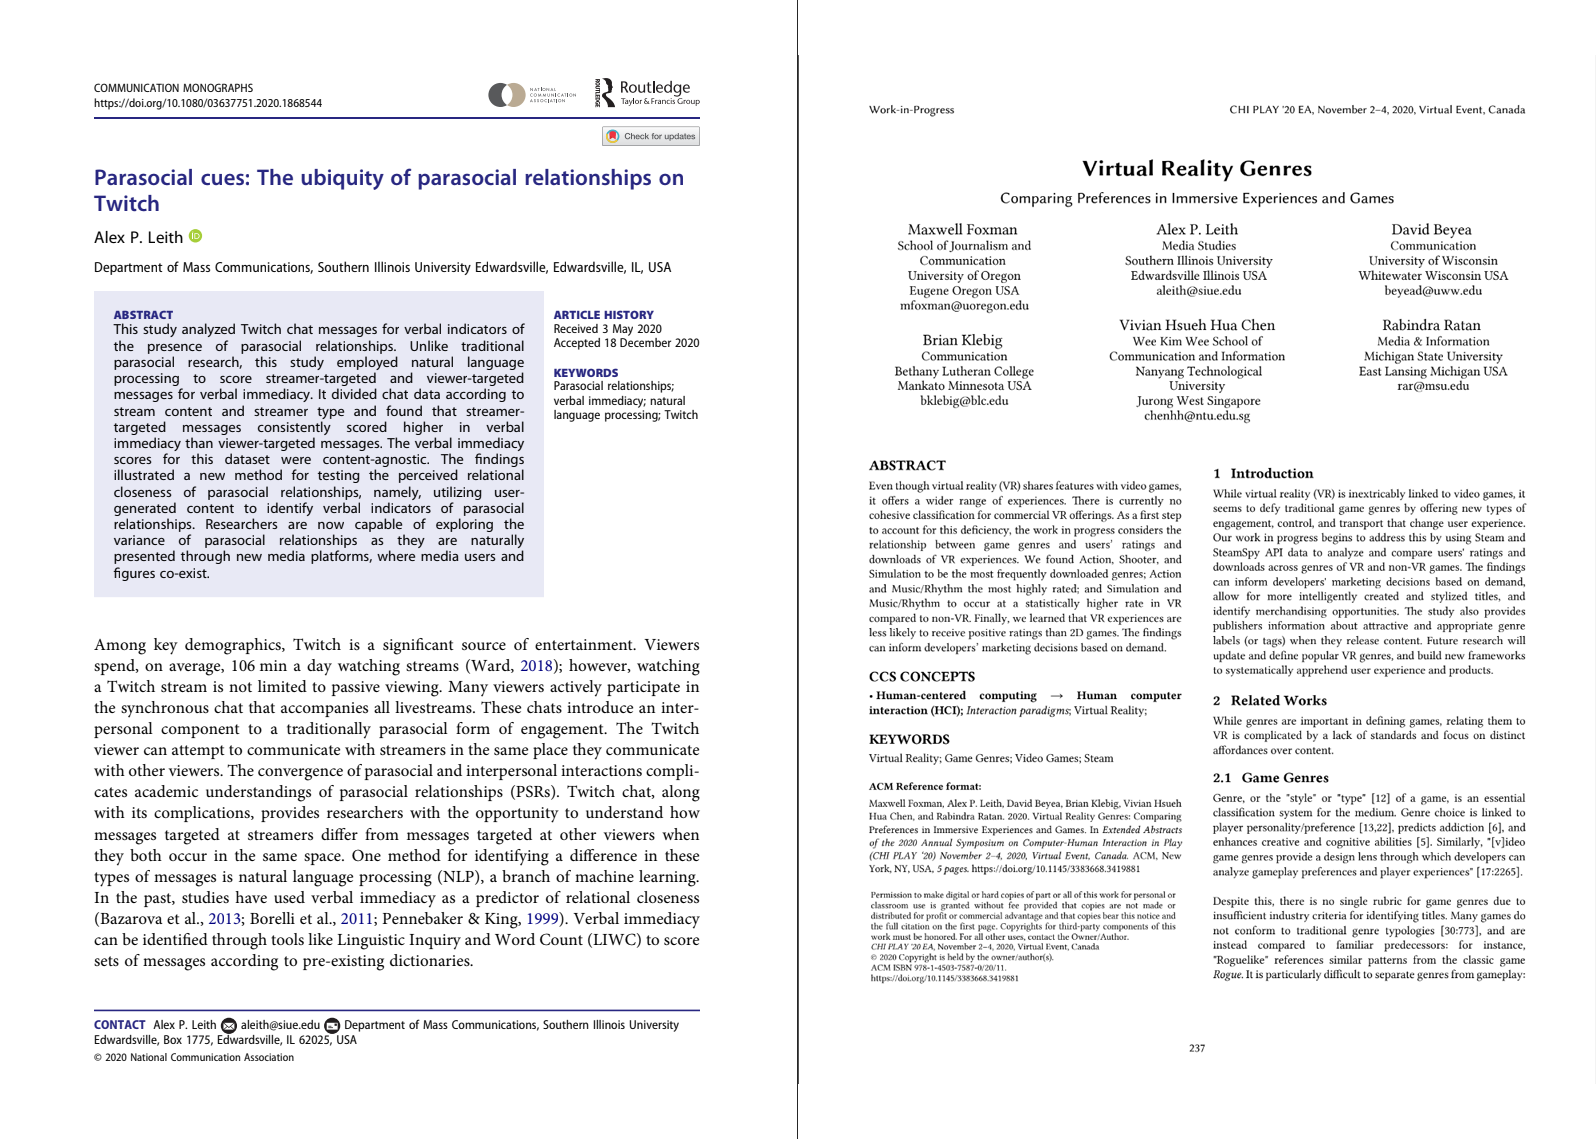
\includegraphics[width=1\textwidth,height=\textheight]{images/papers.png}

\textbf{Theses and dissertations}: Theses and dissertations are written by graduate students to complete their degree requirements. They are typically longer and more comprehensive than research papers.

\textbf{Books}: Books are another way to report research. They are typically written by experts in a particular field and can be a good way to communicate research to a wider audience.

\textbf{Reports}: Reports are written for a specific audience, such as a government agency or a business. They are typically shorter than research papers and focus on a specific topic.

\textbf{Presentations}: Presentations are a way to share research with a live audience. They can be given at conferences, workshops, or other events.

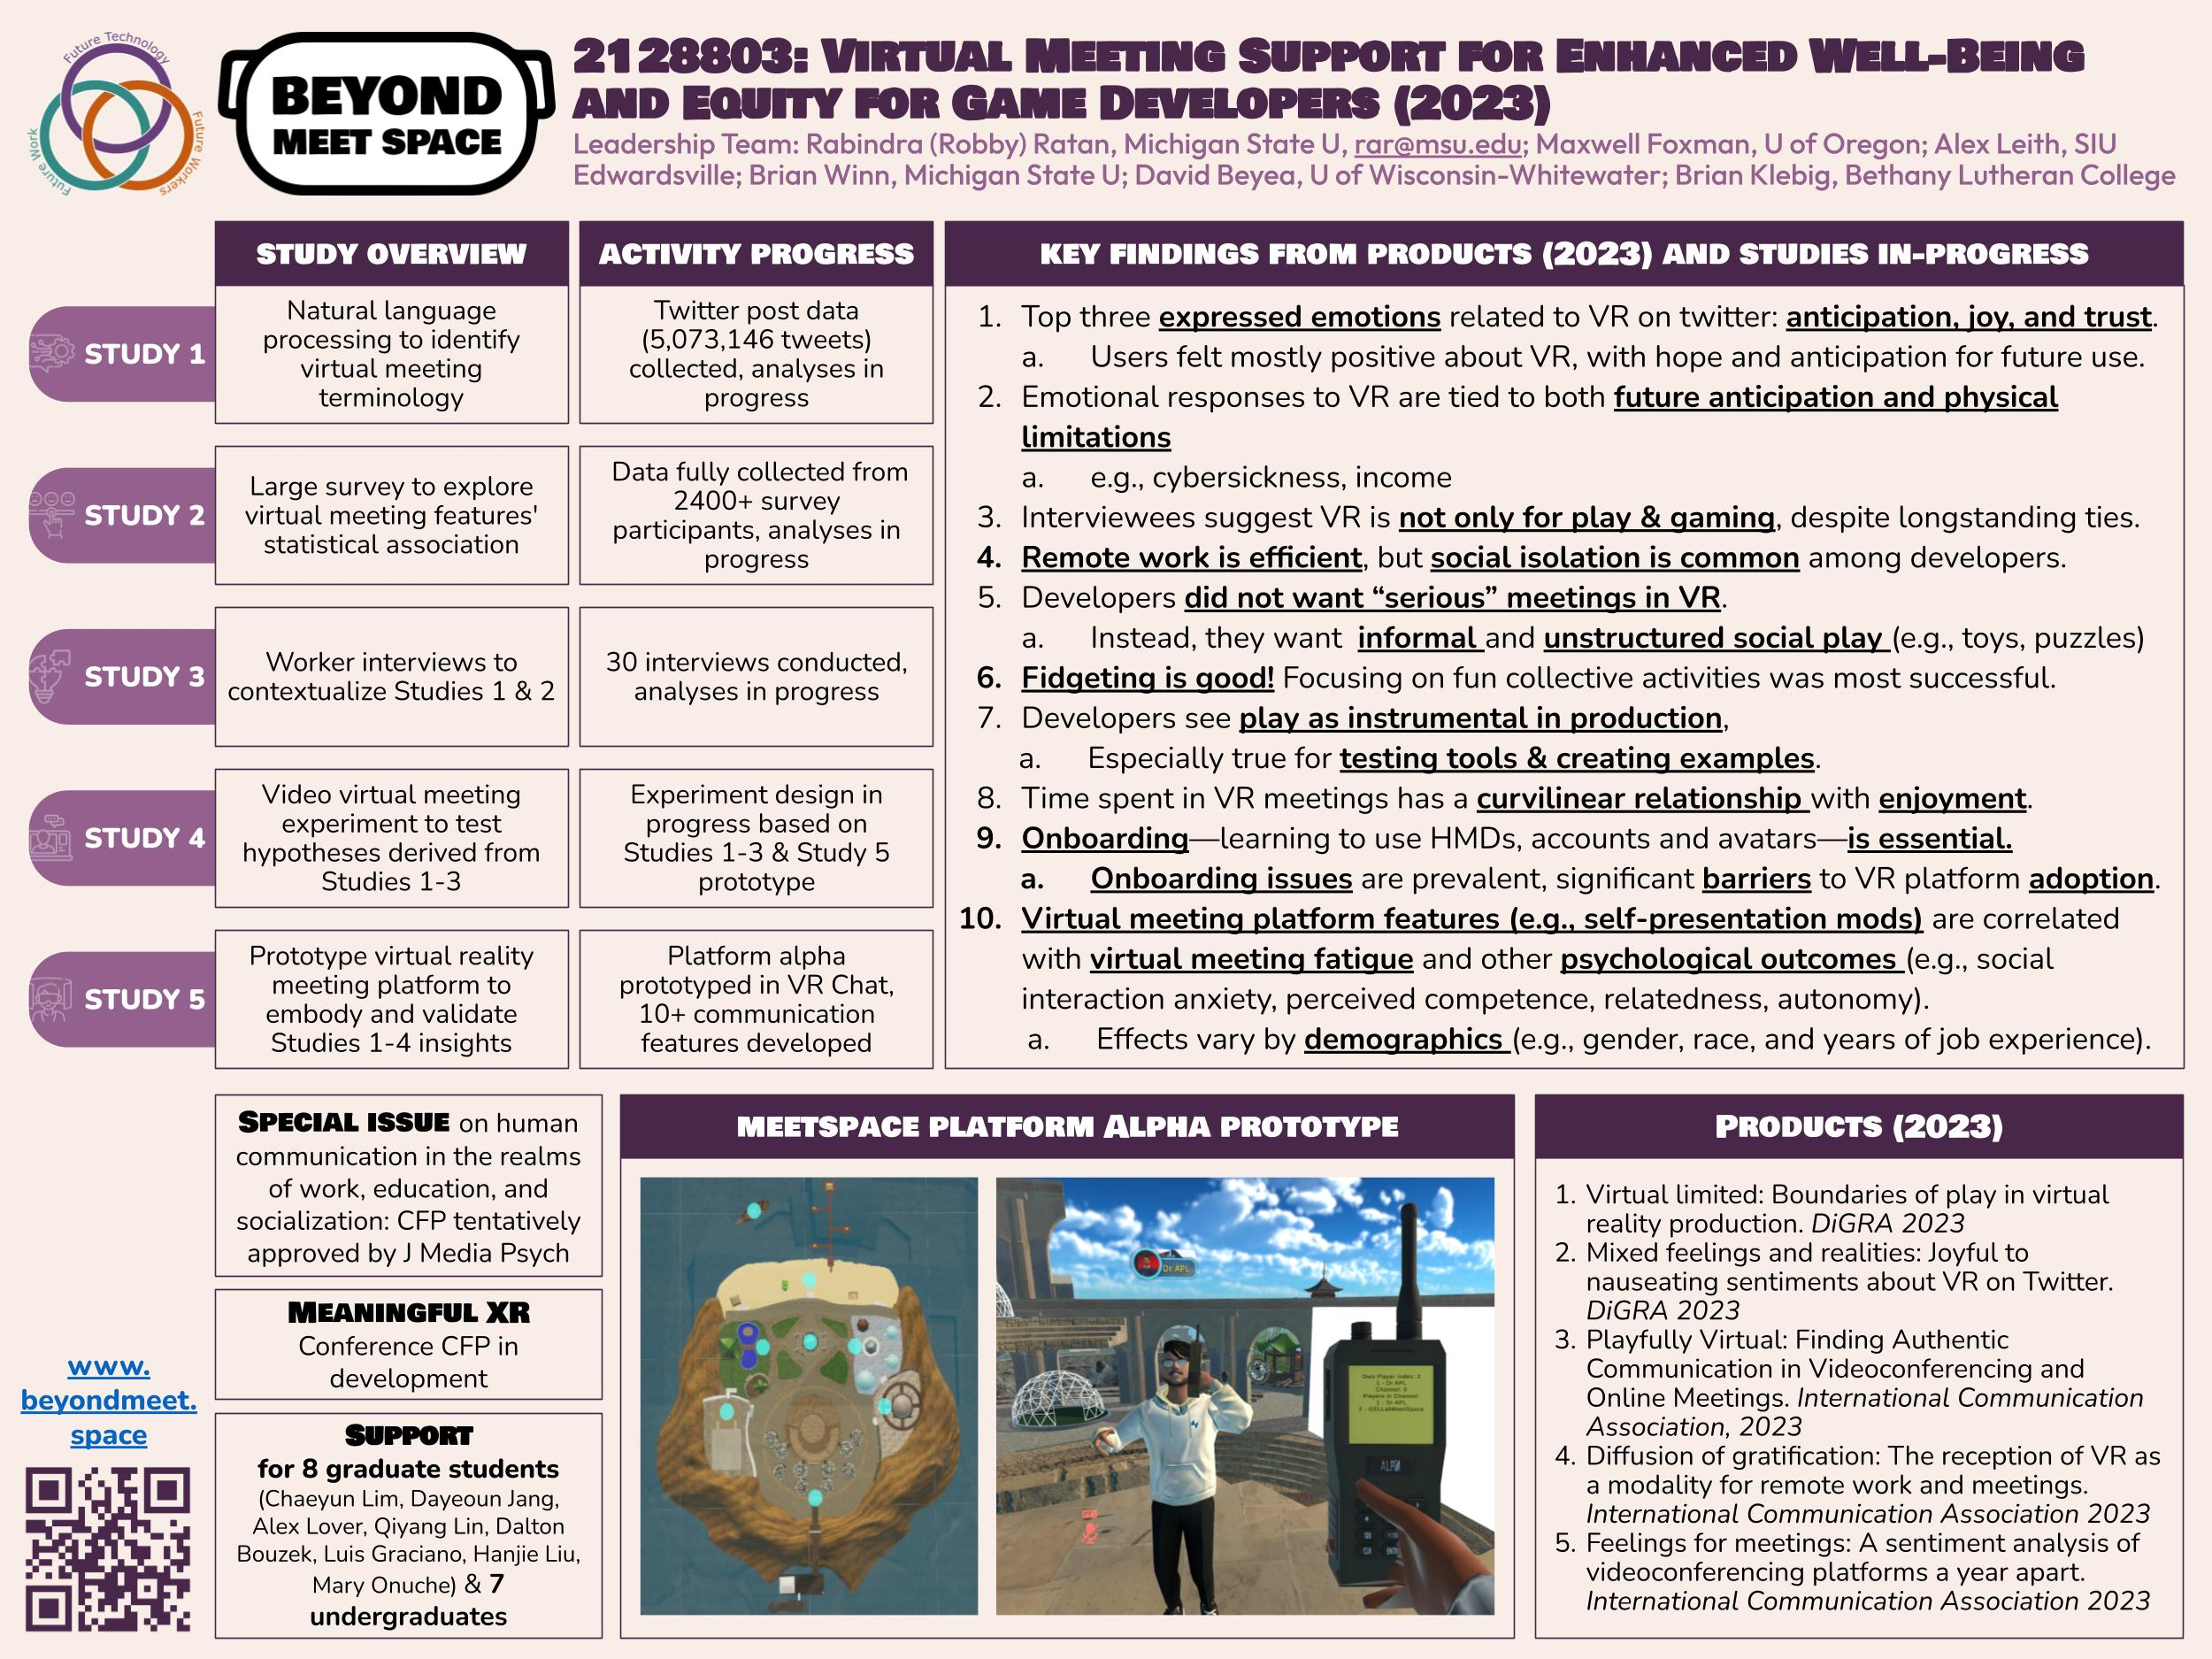
\includegraphics[width=1\textwidth,height=\textheight]{images/BMS 2023 poster final.jpg}

\textbf{Blogs and social media}: Blogs and social media can be used to share research with a wider audience. They are a good way to communicate research in a more informal way.

The best way to report research depends on the specific research project and the intended audience. However, all of these methods can be effective ways to communicate research findings and to contribute to the academic community.

\hypertarget{industry-examples}{%
\subsection*{Industry Examples}\label{industry-examples}}
\addcontentsline{toc}{subsection}{Industry Examples}

There are many different ways to report research in industry. Some of the most common methods include:

\textbf{White papers}: White papers are a type of report that is commonly used in industry to present research findings to a specific audience. They are typically written in a clear and concise style and focus on a specific topic.


\includegraphics[width=1\textwidth,height=\textheight]{images/white_paper.png}

\textbf{Executive summaries}: Executive summaries are a brief overview of a white paper or other research report. They are typically written for senior executives and other decision-makers.

\textbf{Presentations}: Presentations are a way to share research findings with a live audience. They can be given at company meetings, conferences, or other events.

\textbf{Blogs and social media}: Blogs and social media can be used to share research findings with a wider audience. They are a good way to communicate research in a more informal way.

\textbf{Press releases}: Press releases are a way to share research findings with the media. They are typically written in a clear and concise style and focus on the key findings of the research.

\textbf{Technical reports}: Technical reports are a detailed document that describes the research methods and findings. They are typically written for a technical audience.

The best way to report research in industry depends on the specific research project and the intended audience. However, all of these methods can be effective ways to communicate research findings and to contribute to the industry community.

\hypertarget{sections-of-an-academic-paper}{%
\subsection*{Sections of an Academic Paper}\label{sections-of-an-academic-paper}}
\addcontentsline{toc}{subsection}{Sections of an Academic Paper}

\textbf{Title:} The title should be clear, concise, and informative. It should accurately reflect the main topic of the paper and be interesting enough to grab the reader's attention. When titling a paper, it should be no more than 12 words. You only capitalize the first words and proper nouns. If you include a semi-colon, the first word after the semi-colon is considered a first word. You should also bold, center, and double-space the title.

\textbf{Abstract:} The abstract should be concise and informative, summarizing the main points of the paper in a way that is easy to understand. It should be written in the past tense and should not include any citations. The abstract should be a concise and informative summary of the paper, typically 150-250 words long. It should state the purpose of the study, the methods used, the main findings, and the conclusions.

\textbf{Introduction:} The introduction should provide background information on the topic, define the research problem, and state the research question or hypothesis. It should also provide a brief overview of the paper's organization. You should also include an overview of the structure of your paper, including key findings.

\textbf{Literature review:} The literature review should discuss the relevant research that has been done on the topic. It should identify the gaps in the literature and explain how the current study will contribute to knowledge. The literature review should be objective and should not include any personal opinions or biases.

\textbf{Methods:} The methods section should describe how the research was conducted. It should include information on the participants, the materials and procedures used, and the data analysis methods. The methods section should be clear and concise, and should be written in the past tense.

\textbf{Results:} The results section should present the findings of the study. It should be organized and easy to follow, and should use tables and figures to illustrate the data. The results section should be objective and should not include any interpretations or conclusions.

\textbf{Discussion:} The discussion section should interpret the results of the study and relate them to the literature. It should also discuss the limitations of the study and suggest directions for future research. The discussion section should be thoughtful and insightful, and should be written in the present tense.

\textbf{References:} The references section should list all of the sources that were cited in the paper. It should be formatted according to the style guide that is being used (e.g., APA, MLA, Chicago).

\hypertarget{cite}{%
\section{How to Cite Research Papers}\label{cite}}

\hypertarget{why-citing-is-important}{%
\subsection{Why Citing is Important}\label{why-citing-is-important}}

Citing sources in a research article serves several critical purposes. Firstly, it is a matter of academic integrity and ethical conduct. When you cite sources, you give credit to the original authors and researchers whose work has informed or influenced your own. This acknowledgment is not just a formality but a way to show respect for the intellectual contributions of others. Failing to give proper credit can lead to accusations of plagiarism, a serious breach of academic ethics.

Secondly, proper citation helps you avoid plagiarism by clearly distinguishing between your own ideas and those borrowed from others. Plagiarism can have severe consequences, both academically and professionally, tarnishing your reputation and credibility.

Citations also play a crucial role in supporting the claims and arguments presented in your research. By referencing reputable sources, you provide evidence and credibility to your work, enhancing its persuasiveness and reliability. This helps readers assess the validity of your assertions and the strength of your research.

Furthermore, citing sources connects your research to the broader academic discourse. It demonstrates how your work fits into the existing body of knowledge and contributes to the advancement of your field. This contextualization is essential for readers to understand the significance and relevance of your research.

Proper citations facilitate the peer review process, a cornerstone of academic research. When your sources are accurately cited, reviewers can assess the quality and reliability of your research more effectively. This transparency is crucial for maintaining the standards of academic rigor.

Citations also provide readers with the opportunity to delve deeper into related concepts, methodologies, and findings by referring to the cited sources. This additional context can enrich their understanding of your research and encourage further exploration.

Ethically, citing sources is a fundamental responsibility in research. It demonstrates your commitment to conducting honest and responsible research, adhering to established ethical standards in your field. It also promotes transparency and accountability in the dissemination of knowledge.

In addition to ethical considerations, proper citation helps prevent the spread of misinformation. By referencing credible sources, you ensure that the information presented in your research is accurate and trustworthy, contributing to the overall quality of scholarly work.

Finally, citing a range of sources acknowledges the diversity of perspectives and ideas within your field. This inclusivity enriches your research, demonstrating a comprehensive understanding of the subject matter and showing that you have considered various viewpoints.

In conclusion, citing sources in a research article is not just a technical requirement; it is a fundamental practice that upholds academic integrity, supports your arguments, connects your work to the academic community, and contributes to the responsible dissemination of knowledge.

\hypertarget{two-types-in-apa}{%
\subsection*{Two Types in APA}\label{two-types-in-apa}}
\addcontentsline{toc}{subsection}{Two Types in APA}

The American Psychological Association (APA) style is a popular format for citing sources in academic papers. Here are the basic steps on how to cite research papers using APA:

\textbf{In-text citations.}

In-text citations are used to give credit to the sources you used in your paper. They are placed in parentheses after the information you are citing, and they include the author's last name, the year of publication, and the page number(s) where the information can be found. For example, if you are citing a quote from a book by John Smith, published in 2023, on page 100, your in-text citation would look like this: (Smith, 2023, p.~100).

\textbf{Reference list.}

The reference list is a list of all the sources you used in your paper. It is placed at the end of your paper, and it is organized alphabetically by the author's last name. Each entry in the reference list includes the author's name, the year of publication, the title of the source, the publication information, and any other relevant information. For example, the reference list entry for the book by John Smith would look like this:

\begin{quote}
Smith, J. (2023). \emph{The Psychology of Learning}. New York, NY: Oxford University Press.
\end{quote}

Here is the template for each of the typical types of APA citations. Please review the APA website or Purdue's Writing Lab (OWL) for additional help with APA 7th.

\textbf{\emph{Book.}}

Author, A. A. (Year of publication). \emph{Title of work: Capital letter also for subtitle}. Publisher Name. DOI (if available)

\textbf{\emph{Chapter in an Edited Book.}}

Author, A. A., \& Author, B. B. (Year of publication). Title of chapter. In E. E. Editor \& F. F. Editor (Eds.), \emph{Title of work: Capital letter also for subtitle} (pp.~pages of chapter). Publisher.~DOI (if available)

\textbf{\emph{Journal article.}}

Lastname, F. M., \& Lastname, F. M. (Year). Title of article. \emph{Title of Periodical, Vol.(}Issue), page numbers. DOI

\textbf{\emph{Website.}}

Lastname, F. M. (Year, Month Date). \emph{Title of page}. Site name. URL

\textbf{\emph{Dissertation.}}

Lastname, F. M. (Year). \emph{Title of dissertation/thesis} (Publication No.) {[}Doctoral dissertation/Master's thesis, Name of Institution Awarding the Degree{]}. Database or Archive Name.

\textbf{\emph{Report by Government Agency.}}

Organization Name. (Year). \emph{Title of report.} URL

\textbf{\emph{Report by Individual.}}

Lastname, F. M., \& Lastname, F. M. (Year). \emph{Title of report}. Organization Name. URL

\textbf{\emph{Tweet.}}

Lastname, F. M. or Name of Group {[}@username{]}. (Year, Month Date).~\emph{Content of the post up to the first 20 words}{[}Tweet{]}. Site Name. URL

\hypertarget{additional-tips-1}{%
\subsection*{Additional Tips}\label{additional-tips-1}}
\addcontentsline{toc}{subsection}{Additional Tips}

Here are some additional tips for citing research papers using APA:

\textbf{Use a consistent style.}

Using a consistent citation style in a research paper is crucial for several reasons. Firstly, it enhances the readability and professionalism of your work by ensuring uniform formatting throughout the paper, making it easier for readers to find and understand source information. This consistency contributes to a polished and credible presentation. Secondly, it demonstrates your competence and attention to detail as a researcher, showcasing your commitment to following established conventions, which is vital when submitting work to journals or academic institutions with specific style requirements. Moreover, a uniform citation style fosters clarity in academic communication, eliminating confusion caused by variations in formats. It also aids in the peer review process, helping reviewers assess citations efficiently and promoting fairness and transparency in academic discourse. Lastly, it saves time and effort in writing and editing, making it especially valuable for larger research projects. In summary, consistent citation style improves readability, professionalism, and clarity, demonstrates competence, aids in peer review, fosters fairness and transparency, and streamlines the research process, enhancing the overall quality and credibility of your work.

\textbf{Carefully check your citations.}

Careful citation checking in academic and research writing is vital for several reasons. Firstly, it upholds scholarly integrity by preventing plagiarism and ensuring proper attribution to original sources. This practice helps avoid severe academic and professional consequences associated with ethical breaches. Secondly, it enhances the credibility of your work by providing evidence and support for your claims through accurate citations, fostering trust among readers. Thirdly, meticulous citation checking improves the clarity and coherence of your writing, benefiting peer reviewers and readers alike. Additionally, it ensures adherence to specific style guidelines, reflecting attention to detail and professionalism. Checking citations also plays a role in preventing the spread of misinformation, contributing to responsible knowledge dissemination and field integrity. Lastly, it serves as a practical step in the editing process, allowing for error correction and showcasing your commitment to high-quality research. In sum, citation checking is a fundamental practice that supports academic integrity, credibility, readability, adherence to guidelines, misinformation prevention, and overall research quality.

\textbf{Use a citation management tool.}

Citation management software provides several benefits for researchers and scholars. It simplifies the organization and formatting of citations, making it easier to collect and manage references from various sources. This saves time and reduces the risk of errors in citations and bibliographies. The software also automates citation and bibliography formatting according to different styles, streamlining the process and ensuring consistency. Collaboration is facilitated through features for sharing reference libraries, enhancing productivity for team projects. Integration with word processing software simplifies citation insertion and bibliography generation. Additionally, the software can import citation information from databases, keeping you updated with the latest research. Backup and synchronization features ensure the security and accessibility of your reference library across devices.

\hypertarget{communication-theories-1}{%
\chapter{Communication Theories}\label{communication-theories-1}}

\hypertarget{agenda-setting-theory}{%
\section{Agenda Setting Theory}\label{agenda-setting-theory}}

Agenda setting theory is a communication theory that examines the relationship between the media and public opinion. The theory suggests that the media does not simply reflect public opinion, but rather shapes it by determining which issues are considered important. This is done by selecting and highlighting certain news stories over others, and by framing those stories in a particular way.

The theory was first proposed by Maxwell McCombs and Donald Shaw in their 1972 study of the 1968 US presidential election. They found that the media's coverage of the election had a significant impact on the public's perception of the relative importance of the issues. For example, the media focused heavily on the Vietnam War, which led to the public viewing this issue as more important than other issues, such as the economy.

Since then, agenda setting theory has been applied to a wide range of issues, including politics, social problems, and consumer products. The theory has been supported by a number of studies, but it is not without its critics. Some argue that the media does not have as much influence on public opinion as the theory suggests, and that other factors, such as personal experience and social interaction, are more important.

Despite these criticisms, agenda setting theory remains one of the most influential theories in mass communication. It has helped to explain how the media can shape public opinion, and it has implications for the way we think about the role of the media in society.

\textbf{Levels of agenda setting}

There are two levels of agenda setting:

\begin{itemize}
\item
  \textbf{First-level agenda setting}:~This level focuses on the media's ability to influence the salience of issues. Salience refers to the importance or prominence that people attach to an issue. The media can influence salience by selecting and highlighting certain issues over others.
\item
  \textbf{Second-level agenda setting}:~This level focuses on the media's ability to influence the public's perception of the attributes of an issue. This includes the causes, consequences, and solutions to the issue. The media can influence the public's perception of these attributes by the way they frame the issue in their news coverage.
\end{itemize}

\textbf{Factors affecting agenda setting}

There are a number of factors that can affect agenda setting, including:

\begin{itemize}
\item
  \textbf{The media's own agenda}: The media has its own agenda, which is influenced by a variety of factors, such as the ownership of the media outlet, the political climate, and the economic interests of the media.
\item
  \textbf{The public's agenda}: The public also has its own agenda, which is influenced by a variety of factors, such as personal experiences, social interaction, and the media.
\item
  \textbf{The political system}: The political system can also affect agenda setting by setting the agenda for public debate.
\item
  \textbf{The newsworthiness of the issue}: The newsworthiness of an issue is also a factor in agenda setting. Issues that are considered to be more newsworthy are more likely to be covered by the media.
\end{itemize}

\textbf{Conclusion}

Agenda setting theory is a complex and nuanced theory that has been the subject of much research and debate. However, it remains one of the most important theories in mass communication, and it has helped to explain how the media can shape public opinion.

\textbf{References}

\begin{itemize}
\item
  McCombs, M. E., \& Shaw, D. L. (1972). The agenda-setting function of mass media.~\emph{Public Opinion Quarterly, 36}(2), 176-187. \url{doi:10.1086/267990}
\item
  Dearing, J. W., \& Rogers, E. M. (1996). Agenda-setting. In M. B. Salwen \& D. W. Stacks (Eds.),~\emph{An introduction to mass communication theory}~(pp.~125-149). New York, NY: M. E. Sharpe.
\item
  Scheufele, D. A. (1999). Framing as a theory of media effects.~\emph{Journal of Communication, 49}(1), 103-122. \url{doi:10.1111/j.1460-2466.1999.tb02823.x}
\item
  Vliegenthart, R., \& Walgrave, S. (2008). The contingent nature of agenda setting: How political parties affect the salience of issues in government agendas.~\emph{Journal of Politics, 70}(4), 1111-1134. \url{doi:10.1017/S0022381608000363}
\item
  Chong, D., \& Druckman, J. N. (2010). Framing public opinion: How citizens react to elite communications.~\emph{Annual Review of Political Science, 13}, 103-126. \url{doi:10.1146/annurev.polisci.13.042009.102515}
\end{itemize}

\hypertarget{cognitive-dissonance}{%
\section{Cognitive Dissonance}\label{cognitive-dissonance}}

Cognitive dissonance is a state of discomfort that occurs when a person holds two conflicting beliefs, or when a person's behavior is inconsistent with their beliefs. This discomfort motivates the person to try to reduce the dissonance by changing one of the beliefs, changing their behavior, or finding a way to justify the inconsistency.

The theory of cognitive dissonance was first proposed by Leon Festinger in 1957. Festinger argued that people have a need for consistency in their thoughts, beliefs, and behaviors. When this consistency is threatened, people experience cognitive dissonance and are motivated to reduce it.

There are a number of ways that people can reduce cognitive dissonance. One way is to change one of the beliefs. For example, if a person believes that smoking is bad for their health, but they continue to smoke, they might start to believe that smoking is not as bad as they thought it was.

Another way to reduce cognitive dissonance is to change one's behavior. For example, if a person believes that they should eat healthy, but they continue to eat unhealthy foods, they might start to eat healthier foods.

Finally, people can also reduce cognitive dissonance by finding a way to justify the inconsistency. For example, a smoker might justify their smoking by saying that they enjoy it and that it helps them to relax.

Cognitive dissonance is a powerful motivator of human behavior. It can lead people to change their beliefs, their behaviors, or their justifications for their behavior. It can also lead to a number of other consequences, such as anxiety, stress, and depression.

Here are some examples of cognitive dissonance:

\begin{itemize}
\item
  A person who believes in saving money but spends all of their disposable income on unnecessary items.
\item
  A person who believes in being honest but cheats on their taxes.
\item
  A person who believes in eating healthy but eats junk food all the time.
\item
  A person who believes in animal rights but wears leather shoes.
\end{itemize}

These are just a few examples of how cognitive dissonance can manifest itself in our everyday lives. It is important to note that cognitive dissonance is not always negative. In some cases, it can motivate us to change our behavior for the better. For example, a person who experiences cognitive dissonance after smoking a cigarette might be more likely to quit smoking.

Cognitive dissonance is a complex phenomenon that has been studied by psychologists for many years. It is a powerful force that can have a significant impact on our thoughts, beliefs, and behaviors.

\textbf{References}

\begin{itemize}
\item
  Festinger, L. (1957).~\emph{A theory of cognitive dissonance}. Stanford, CA: Stanford University Press.
\item
  Cooper, J., \& Fazio, R. H. (1984). A new look at dissonance theory. In L. Berkowitz (Ed.),~\emph{Advances in experimental social psychology}~(Vol. 17, pp.~229-266).~New York, NY: Academic Press.
\item
  Harmon-Jones, E. (2002). Cognitive dissonance theory: Current status and controversies. In M. P. Zanna (Ed.),~\emph{Advances in experimental social psychology}~(Vol. 34, pp.~1-57). New York, NY: Academic Presss
\item
  Stone, J., \& Fernandez, G. (2016). Cognitive dissonance.~\emph{Current Opinion in Psychology, 11}, 100-105. \url{doi:10.1016/j.copsyc.2016.02.002}
\end{itemize}

\hypertarget{cultivation-theory}{%
\section{Cultivation Theory}\label{cultivation-theory}}

Cultivation theory is a communication theory that examines the long-term effects of television viewing on viewers' conceptions of social reality. The theory was developed by George Gerbner and his colleagues at the University of Pennsylvania's Annenberg School for Communication in the 1960s.

Cultivation theory proposes that heavy television viewers come to see the world in a way that is consistent with the images and messages that they are repeatedly exposed to on television. This is because television is a powerful socializing agent that can shape our beliefs, attitudes, and values.

The theory has been supported by a number of studies, which have found that heavy television viewers are more likely to overestimate the likelihood of violence, crime, and danger in the world. They are also more likely to have a pessimistic view of human nature and to be fearful of strangers.

Cultivation theory has been criticized for being too simplistic and for failing to take into account other factors that can influence our perceptions of reality, such as personal experience and social interaction. However, the theory remains an important framework for understanding the effects of television on our lives.

Here are some of the key concepts of cultivation theory:

\begin{itemize}
\item
  \textbf{Symbolic environment}:~The world of television, as presented to viewers.
\item
  \textbf{Cultivation effect}:~The process by which heavy television viewing leads to viewers' perceptions of reality becoming more consistent with the images and messages presented on television.
\item
  \textbf{Mainstreaming}:~The tendency for heavy television viewers to come to share similar perceptions of reality, regardless of their demographic characteristics.
\item
  \textbf{Resonance}:~The process by which the cultivation effect is stronger for viewers who are already predisposed to believe the messages that are presented on television.
\end{itemize}

Cultivation theory has been applied to a wide range of topics, including violence, crime, fear, gender roles, and political attitudes. The theory has also been used to examine the effects of other media, such as the internet and video games.

Cultivation theory is a complex and nuanced theory that has been the subject of much research and debate. However, it remains one of the most important theories in mass communication, and it has helped to explain how television can shape our perceptions of reality.

\textbf{References}

\begin{itemize}
\item
  Gerbner, G., Gross, L., Morgan, M., \& Signorielli, N. (1986). Living with television: The dynamics of the cultivation process.~\emph{Communication Research, 13}(4), 373-398. \url{doi:10.1177/009365086013004001}
\item
  Morgan, M., \& Shanahan, J. (1997). Television and the cultivation of values: A 20-year assessment.~\emph{Communication Research, 24}(5), 367-399. \url{doi:10.1177/009365097024005001}
\item
  Shrum, L. J. (2004). Media consumption and perceptions of social reality: A cultivation perspective. In J. Bryant \& D. Zillmann (Eds.),~\emph{Media effects: Advances in theory and research}~(pp.~41-65). Mahwah, NJ: Lawrence Erlbaum Associates.
\item
  Potter, W. J. (2011).~\emph{Media literacy}~(9th ed.). Thousand Oaks, CA: Sage.
\end{itemize}

\hypertarget{elaboration-likelihood-model}{%
\section{Elaboration Likelihood Model}\label{elaboration-likelihood-model}}

The elaboration likelihood model (ELM) is a dual-process theory of persuasion that was developed by Richard E. Petty and John Cacioppo in 1980. The ELM proposes that there are two routes to persuasion: the central route and the peripheral route.

The central route is a high-effort route to persuasion that involves carefully considering the message and evaluating the arguments presented. This route is more likely to be used when people are motivated and have the ability to think critically about the message.

The peripheral route is a low-effort route to persuasion that involves relying on superficial cues, such as the source of the message or the way it is presented. This route is more likely to be used when people are not motivated or do not have the ability to think critically about the message.

The ELM suggests that the effectiveness of a persuasive message depends on the route that is used. Messages that are processed through the central route are more likely to lead to lasting attitude change, while messages that are processed through the peripheral route are more likely to lead to temporary attitude change.

The ELM has been supported by a number of studies, and it has been used to explain a wide range of persuasion phenomena, such as the effects of advertising, political campaigns, and social movements.

Here are some of the key concepts of the ELM:

\begin{itemize}
\item
  \textbf{Elaboration}:~The amount of cognitive effort that is put into processing a message.
\item
  \textbf{Motivation}:~The desire to process a message in a thoughtful and unbiased way.
\item
  \textbf{Ability}:~The ability to process a message in a thoughtful and unbiased way.
\item
  \textbf{Peripheral cues}:~Superficial cues that are used to evaluate a message, such as the source of the message or the way it is presented.
\item
  \textbf{Central route to persuasion}:~A high-effort route to persuasion that involves carefully considering the message and evaluating the arguments presented.
\item
  \textbf{Peripheral route to persuasion}:~A low-effort route to persuasion that involves relying on superficial cues, such as the source of the message or the way it is presented.
\end{itemize}

The ELM is a complex and nuanced theory that has been the subject of much research and debate. However, it remains one of the most important theories in persuasion research, and it has helped to explain how people are persuaded by messages.

\textbf{References}

\begin{itemize}
\item
  Petty, R. E., \&~Cacioppo, J. T. (1986). The elaboration likelihood model of persuasion.~\emph{Advances in Experimental Social Psychology, 19}, 123-205. \url{doi:10.1016/S0065-2601(08)60214-2}
\item
  Petty,~R. E., \& Cacioppo, J. T. (1996).~\emph{Attitude change: Classic and contemporary approaches}. New York, NY: McGraw-Hill.
\item
  Chaiken, S. (1980). Heuristic versus systematic processing of persuasive messages: Evidence of two routes to persuasion. \_In J. T. Cacioppo \& R. E. Petty (Eds.),~\emph{Social cognition: The Ontario symposium on personality and social psychology}~(Vol. 1, pp.~212-252). Hillsdale, NJ: Erlbaum.
\end{itemize}

\hypertarget{framing-theory}{%
\section{Framing Theory}\label{framing-theory}}

Framing theory is a communication theory that examines how the way an issue is presented can affect how people understand and respond to it. The theory was first proposed by Erving Goffman in 1974, and it has been used to explain a wide range of phenomena, such as the effects of news coverage on public opinion, the impact of advertising on consumer behavior, and the role of social movements in shaping public discourse.

Framing theory suggests that the way an issue is presented can shape how people think about it by influencing the following:

\begin{itemize}
\item
  \textbf{The salience of the issue}:~The extent to which the issue is noticed and remembered.
\item
  \textbf{The definition of the issue}:~The way the issue is understood and interpreted.
\item
  \textbf{The causal attributions}:~The reasons that are given for the issue.
\item
  \textbf{The moral implications}:~The ethical or moral dimensions of the issue.
\item
  \textbf{The emotional response}:~The feelings that are evoked by the issue.
\end{itemize}

Framing theory has been supported by a number of studies, which have found that the way an issue is framed can have a significant impact on how people think about it and respond to it. For example, studies have shown that the way news stories about crime are framed can affect people's fear of crime, and the way advertising is framed can affect people's purchase decisions.

Framing theory is a complex and nuanced theory that has been the subject of much research and debate. However, it remains an important framework for understanding how the way we communicate about issues can shape how people think about them.

Here are some of the key concepts of framing theory:

\begin{itemize}
\item
  \textbf{Frame}:~A way of presenting an issue that highlights certain aspects of the issue and obscures others.
\item
  \textbf{Framing effects}:~The ways in which the way an issue is framed can affect how people think about it and respond to it.
\item
  \textbf{Framing bias}:~The tendency for people to be more persuaded by messages that are framed in a way that is consistent with their existing beliefs and attitudes.
\item
  \textbf{Framing strategies}:~The techniques that are used to frame issues, such as the use of language, images, and metaphors.
\end{itemize}

Framing theory has been applied to a wide range of topics, including politics, health, the environment, and social justice. The theory has also been used to examine the effects of different media, such as news, advertising, and social media.

Framing theory is a powerful tool for understanding how the way we communicate about issues can shape how people think about them. By understanding how framing works, we can be more mindful of the ways in which our own communication can influence others.

\textbf{References}

\begin{itemize}
\item
  Entman, R. M. (1993). Framing: Toward clarification of a fractured paradigm.~\emph{Journal of Communication, 43}(4), 51-58. \url{doi:10.1111/j.1460-2466.1993.tb01304.x}
\item
  Scheufele, D. A. (1999). Framing as a theory of media effects.~\emph{Journal of Communication, 49}(1), 103-122. \url{doi:10.1111/j.1460-2466.1999.tb02823.x}
\item
  Chong, D., \& Druckman, J. N. (2010). Framing public opinion: How citizens react to elite communications.~\emph{Annual Review of Political Science, 13}, 103-126. \url{doi:10.1146/annurev.polisci.13.042009.102515}
\end{itemize}

\hypertarget{gatekeeping-theory}{%
\section{Gatekeeping Theory}\label{gatekeeping-theory}}

Gatekeeping theory is a communication theory that examines how decisions are made about what news stories get covered and how they are presented. The theory was first proposed by Kurt Lewin in 1947, and it has been used to explain a wide range of phenomena, such as the effects of news coverage on public opinion, the impact of media bias, and the role of journalists in shaping public discourse.

Gatekeeping theory suggests that there are a number of factors that can influence the news selection process, including:

\begin{itemize}
\item
  \textbf{The gatekeepers}:~The people who make decisions about what news stories get covered and how they are presented.
\item
  \textbf{The news values}:~The criteria that are used to determine which news stories are newsworthy.
\item
  \textbf{The media environment}:~The economic, political, and social factors that shape the media.
\item
  \textbf{The audience}:~The people who consume news.
\end{itemize}

Gatekeeping theory has been supported by a number of studies, which have found that the news selection process is often influenced by the gatekeepers' personal biases, the news values of the media organization, and the political and economic climate.

For example, studies have shown that journalists are more likely to cover stories that are consistent with their own political beliefs, and that news organizations are more likely to cover stories that are seen as being in the public interest or that are likely to attract a large audience.

Gatekeeping theory is a complex and nuanced theory that has been the subject of much research and debate. However, it remains an important framework for understanding how decisions are made about what news stories get covered and how they are presented.

Here are some of the key concepts of gatekeeping theory:

\begin{itemize}
\item
  \textbf{Gatekeeper}:~A person who makes decisions about what news stories get covered and how they are presented.
\item
  \textbf{News values}:~The criteria that are used to determine which news stories are newsworthy.
\item
  \textbf{Media environment}:~The economic, political, and social factors that shape the media.
\item
  \textbf{Audience}:~The people who consume news.
\item
  \textbf{Personal bias}:~The personal beliefs and opinions of the gatekeeper.
\item
  \textbf{News organization}:~The media outlet where the gatekeeper works.
\item
  \textbf{Public interest}:~The perceived benefit to the public of covering a particular news story.
\item
  \textbf{Large audience}:~The perceived potential for a news story to attract a large number of viewers or readers.
\end{itemize}

Gatekeeping theory has been applied to a wide range of topics, including politics, health, the environment, and social justice. The theory has also been used to examine the effects of different media, such as news, advertising, and social media.

Gatekeeping theory is a powerful tool for understanding how decisions are made about what news stories get covered and how they are presented. By understanding how gatekeeping works, we can be more mindful of the ways in which our own news consumption can be influenced.

\textbf{References}

\begin{itemize}
\item
  Lewin, K. (1947).~Frontiers in group dynamics: Concept, method and reality in social science; social equilibria and social change.~\emph{Human Relations,~1}(2), 5-41. \url{doi:10.1177/001872674700100201}
\item
  Shoemaker, P. J., \&~Reese, S. D. (1996).~\emph{Mediating the message: Theories of influences on mass media content}~(2nd ed.). New York, NY: Longman.
\item
  Tuchman, G. (1978).~\emph{Making news: A study in the construction of reality}. New York, NY: Free Press.
\end{itemize}

\hypertarget{hyperpersonal-model}{%
\section{Hyperpersonal Model}\label{hyperpersonal-model}}

The hyperpersonal model is a communication theory that examines how computer-mediated communication (CMC) can create more personal and intimate relationships than traditional face-to-face (FtF) communication. The theory was proposed by Joseph Walther in 1992, and it has been used to explain a wide range of phenomena, such as the development of online relationships, the impact of CMC on social interaction, and the role of CMC in shaping our self-presentation.

The hyperpersonal model suggests that CMC can create more personal and intimate relationships than FtF communication because it offers a number of advantages, including:

\begin{itemize}
\item
  \textbf{Attribution ambiguity}:~The sender's physical appearance and nonverbal cues are not available in CMC, which allows the receiver to fill in the gaps with their own interpretations.
\item
  \textbf{Control over self-presentation}:~CMC allows users to control their self-presentation more than FtF communication, which can lead to more favorable impressions.
\item
  \textbf{Attribution confidence}:~CMC users are more likely to believe that they have accurate information about the other person, which can lead to more trust and intimacy.
\item
  \textbf{Interactivity}:~CMC is more interactive than traditional mass media, which allows for more communication and feedback between the sender and receiver.
\end{itemize}

The hyperpersonal model has been supported by a number of studies, which have found that CMC users often report feeling more connected and intimate with their online partners than they do with their FtF partners. For example, one study found that CMC users were more likely to disclose personal information to their online partners than they were to their FtF partners.

However, the hyperpersonal model has also been criticized for being too simplistic and for failing to take into account the role of other factors, such as the individual's personality and the relationship context. Nevertheless, the hyperpersonal model remains an important framework for understanding how CMC can create more personal and intimate relationships than traditional FtF communication.

Here are some of the key concepts of the hyperpersonal model:

\begin{itemize}
\item
  \textbf{Attribution ambiguity}:~The lack of physical cues in CMC can lead to ambiguity about the sender's intentions and personality.
\item
  \textbf{Control over self-presentation}:~CMC allows users to control how they are perceived by others.
\item
  \textbf{Attribution confidence}:~CMC users are more likely to believe that they have accurate information about the other person.
\item
  \textbf{Interactivity}:~CMC allows for more communication and feedback between the sender and receiver.
\item
  \textbf{Hyperpersonal communication}:~Communication that is more personal and intimate than traditional face-to-face communication.
\end{itemize}

The hyperpersonal model has been applied to a wide range of topics, including online dating, online gaming, and social media. The theory has also been used to examine the effects of different CMC technologies, such as email, instant messaging, and social networking sites.

The hyperpersonal model is a powerful tool for understanding how CMC can create more personal and intimate relationships than traditional FtF communication. By understanding how the hyperpersonal model works, we can be more mindful of the ways in which our own CMC interactions can be shaped.

\textbf{References}

\begin{itemize}
\item
  Walther, J. B. (1992). Interpersonal effects in computer-mediated communication:~A relational perspective.~\emph{Communication Research, 19}(1), 52-90.~\url{doi:10.1177/009365092019001003}
\item
  Walther, J. B. (1996). Computer-mediated communication: Impersonal, interpersonal, and hyperpersonal interaction.~\emph{Communication Research, 23}(1), 3-43. \url{doi:10.1177/009365096023001001}
\item
  Walther,~J. B. (2007). Selective self-presentation in computer-mediated communication: Hyperpersonal dimensions of technology, language, and~the self.~\emph{Computers in Human Behavior, 23}(5), 2637-2653. \url{doi:10.1016/j.chb.2005.10.014}
\end{itemize}

\hypertarget{knowledge-gap-hypothesis}{%
\section{Knowledge Gap Hypothesis}\label{knowledge-gap-hypothesis}}

The knowledge gap hypothesis (KGH) is a communication theory that predicts that the gap in knowledge between the informed and the uninformed will widen over time, rather than close, as a result of mass communication. The theory was first proposed by Philip J. Tichenor, George A. Donohue, and Clarice N. Olien in 1970, and it has been used to explain a wide range of phenomena, such as the effects of news coverage on public opinion, the impact of educational campaigns, and the role of the media in shaping social inequality.

The KGH suggests that the gap in knowledge between the informed and the uninformed will widen over time because of the following factors:

\begin{itemize}
\item
  \textbf{Differential access to information}:~People with higher socioeconomic status (SES) are more likely to have access to information, such as through education, the media, and social networks.
\item
  \textbf{Differential motivation to learn}:~People with higher SES are more likely to be motivated to learn about new information, such as because they are more likely to be involved in civic activities or to have a need for the information.
\item
  \textbf{Differential ability to understand information}:~People with higher SES are more likely to be able to understand and retain new information, such as because they have more cognitive resources or because they are more familiar with the language and concepts used in the information.
\end{itemize}

The KGH has been supported by a number of studies, which have found that the gap in knowledge between the informed and the uninformed does indeed widen over time. For example, one study found that the gap in knowledge about climate change between people with high and low levels of education widened over a period of 15 years.

However, the KGH has also been criticized for being too simplistic and for failing to take into account the role of other factors, such as the individual's motivation and the nature of the information. Nevertheless, the KGH remains an important framework for understanding how mass communication can contribute to social inequality.

Here are some of the key concepts of the knowledge gap hypothesis:

\begin{itemize}
\item
  \textbf{Knowledge gap}:~The difference in knowledge between the informed and the uninformed.
\item
  \textbf{Mass communication}:~The process of sending messages to a large audience through the media.
\item
  \textbf{Socioeconomic status (SES)}:~A measure of a person's social and economic position, such as their income, education, and occupation.
\item
  \textbf{Differential access to information}:~The unequal distribution of information among different groups of people.
\item
  \textbf{Differential motivation to learn}:~The different levels of motivation that people have to learn new information.
\item
  \textbf{Differential ability to understand information}:~The different levels of ability that people have to understand and retain new information.
\end{itemize}

The KGH has been applied to a wide range of topics, such as public health, education, and politics. The theory has also been used to examine the effects of different media, such as news, advertising, and social media.

The KGH is a powerful tool for understanding how mass communication can contribute to social inequality. By understanding how the KGH works, we can be more mindful of the ways in which our own communication can help to widen or narrow the knowledge gap.

\textbf{References}

\begin{itemize}
\item
  Tichenor, P. J., Donohue, G. A., \& Olien, C. N. (1970). Mass media flow and differential growth in knowledge.~\emph{Public Opinion Quarterly, 34}(2),~159-170. \url{doi:10.1086/267856}
\item
  Viswanath, K., \& Finnegan, J. R. (1996). The knowledge gap hypothesis: Twenty-five years later.~\emph{Communication Research, 23}(5), 559-587. \url{doi:10.1177/009365096023005003}
\item
  Weimann, G. (1994). The influentials: People who influence people. New York, NY: Transaction Publishers.
\end{itemize}

\hypertarget{online-disinhibition-effect}{%
\section{Online Disinhibition Effect}\label{online-disinhibition-effect}}

The online disinhibition effect (ODE) is a phenomenon that occurs when people are more likely to say or do things online that they would not say or do in person. The ODE can be attributed to a number of factors, including:

\begin{itemize}
\item
  \textbf{Anonymity}:~When people are anonymous, they are less likely to feel inhibited by social conventions or norms.
\item
  \textbf{Immediacy}:~Online communication is often more immediate than face-to-face communication, which can lead to people saying things without thinking them through.
\item
  \textbf{Absence of cues}:~Online communication lacks many of the social cues that are present in face-to-face communication, such as body language and tone of voice. This can make it difficult to interpret messages and can lead to misunderstandings.
\item
  \textbf{Disinhibition}:~The ODE can also be attributed to a personality trait known as disinhibition, which is the tendency to act without thinking about the consequences.
\end{itemize}

The ODE can have both positive and negative consequences. On the one hand, it can allow people to be more honest and open than they would be in person. This can be beneficial for communication and relationships. On the other hand, the ODE can also lead to cyberbullying, trolling, and other forms of online harassment.

Here are some of the key concepts of the online disinhibition effect:

\begin{itemize}
\item
  \textbf{Anonymity}:~The state of being unknown or unidentifiable.
\item
  \textbf{Immediacy}:~The quality of being happening or occurring at the same time.
\item
  \textbf{Absence of cues}:~The lack of social cues, such as body language and tone of voice, in online communication.
\item
  \textbf{Disinhibition}:~The tendency to act without thinking about the consequences.
\item
  \textbf{Online disinhibition effect (ODE)}:~The phenomenon that occurs when people are more likely to say or do things online that they would not say or do in person.
\end{itemize}

The ODE has been studied by psychologists and communication scholars for many years. There is still much that we do not know about the ODE, but it is a phenomenon that is important to understand in order to use online communication safely and effectively.

Here are some of the ways to mitigate the negative effects of the ODE:

\begin{itemize}
\item
  \textbf{Be aware of the ODE}:~The first step to mitigating the negative effects of the ODE is to be aware of it. Once you are aware of the ODE, you can start to think about how it might be affecting your online behavior.
\item
  \textbf{Be mindful of your audience}:~When you are communicating online, it is important to be mindful of your audience. Remember that the people you are communicating with may not be who they say they are.
\item
  \textbf{Think before you post}:~Before you post anything online, take a moment to think about what you are saying and how it might be interpreted.
\item
  \textbf{Use appropriate language}:~Be mindful of the language you use online. Avoid using language that could be offensive or hurtful.
\item
  \textbf{Be respectful}:~Always be respectful of others, even if you disagree with them.
\end{itemize}

The ODE is a complex phenomenon, but by being aware of it and taking steps to mitigate its negative effects, we can use online communication safely and effectively.

\textbf{References}

\begin{itemize}
\item
  Suler, J. (2004). The online disinhibition effect.~\emph{Cyberpsychology \& Behavior, 7}(3), 321-326. \url{doi:10.1089/1094931041291295}
\item
  Joinson, A. N. (2001). Self-disclosure in computer-mediated communication: The role of self-awareness and privacy concerns.~\emph{European Journal of Social Psychology, 31}(2), 177-192. \url{doi:10.1002/ejsp.141}
\item
  Postmes, T., Spears, R., \& Lea, M. (2000). The social psychology of computer-mediated communication.~\emph{Annual Review of Psychology, 51}, 669-703. \url{doi:10.1146/annurev.psych.51.1.669}
\item
  Tanis, M. (2008). Online disinhibition: Implications for understanding computer-mediated communication.~\emph{Computers in Human Behavior, 24}(6), 2253-2260. \url{doi:10.1016/j.chb.2008.02.007}
\item
  McKenna, K. Y. A., \& Bargh, J. A. (1998). In-group affiliation and computer-mediated communication: Group versus individual identity salience.~\emph{Personality and Social Psychology Bulletin, 24}(10), 1095-1105. \url{doi:10.1177/01461672982410006}
\end{itemize}

\hypertarget{parasocial-interaction}{%
\section{Parasocial Interaction}\label{parasocial-interaction}}

Parasocial interaction (PSI) is a term used to describe the illusion of a close relationship between a media persona and a viewer or listener. The term was coined by Donald Horton and Richard Wohl in 1956, who defined it as ``the perception of the performer-audience relationship as involving mutual intimacy.''

PSI can occur in any medium where there is a one-way flow of communication, such as television, radio, and the internet. It is most likely to occur when the media persona is perceived as being attractive, likable, and trustworthy.

There are a number of factors that can contribute to PSI, including:

\begin{itemize}
\item
  \textbf{The amount of exposure}:~The more exposure a person has to a media persona, the more likely they are to develop a parasocial relationship with that persona.
\item
  \textbf{The perceived similarity}:~People are more likely to develop parasocial relationships with media personas who they perceive as being similar to themselves.
\item
  \textbf{The perceived intimacy}:~The more intimate the relationship between the media persona and the viewer or listener is perceived to be, the more likely PSI is to occur.
\end{itemize}

PSI can have both positive and negative consequences. On the one hand, it can provide comfort and companionship for people who are lonely or isolated. On the other hand, it can lead to unrealistic expectations about relationships and can make it difficult to form real-world relationships.

Here are some of the key concepts of parasocial interaction:

\begin{itemize}
\item
  \textbf{Parasocial interaction (PSI)}:~The illusion of a close relationship between a media persona and a viewer or listener.
\item
  \textbf{Media persona}:~A person who is presented to an audience through a media medium.
\item
  \textbf{Viewer or listener}:~A person who consumes media content.
\item
  \textbf{Mutual intimacy}:~The perception that two people share a close and personal relationship.
\item
  \textbf{Unrealistic expectations}:~Expectations that are not based on reality.
\end{itemize}

PSI has been studied by psychologists and communication scholars for many years. There is still much that we do not know about PSI, but it is a phenomenon that is important to understand in order to understand the effects of media on people.

Here are some of the key citations in APA 7th for parasocial interaction:

\begin{itemize}
\item
  Horton,~D., \& Wohl, R. R. (1956). Mass communication and para-social interaction: Observations on intimacy at a distance.~\emph{Psychiatry, 19}(3), 215-229.~\url{doi:10.1176/ps.19.3.215}
\item
  Rubin, A. M. (1977). Relationships between television viewing patterns and social behaviors.~\emph{Communication Research, 4}(1), 19-51. \url{doi:10.1177/009365077004001002}
\item
  Perse, E. M. (1990). Media involvement and other predictors of audience response to televised political advertisements.~\emph{Communication Research, 17}(1), 155-177. \url{doi:10.1177/009365090017001007}
\item
  Giles, D., \& Maltby, J. (2015). The parasocial relationship: A critical review of the literature.~\emph{Communication Research, 42}(6), 752-777. \url{doi:10.1177/0093650214544163}
\item
  Rubin, A. M., \& Rubin, R. B. (2015).~\emph{Communication research: Approaches and methods}~(7th ed.). Boston, MA: Pearson.
\end{itemize}

\hypertarget{social-learning-theory}{%
\section{Social Learning Theory}\label{social-learning-theory}}

Social learning theory is a psychological theory that explains how people learn new behaviors by observing and modeling the behaviors of others. The theory was developed by Albert Bandura in the 1960s, and it has been used to explain a wide range of phenomena, such as the development of aggression, the acquisition of prosocial behaviors, and the impact of media on behavior.

Social learning theory is based on the following assumptions:

\begin{itemize}
\item
  People learn by observing and modeling the behaviors of others.~This is known as observational learning.
\item
  The learning process is influenced by a number of factors, including attention, retention, reproduction, and reinforcement.
\item
  People are more likely to learn behaviors that are rewarded or reinforced.
\item
  People are also more likely to learn behaviors that are performed by people they admire or respect.
\end{itemize}

Social learning theory has been supported by a number of studies, which have found that people are more likely to imitate the behaviors of others when they are paying attention to those behaviors, when they can remember those behaviors, and when they are rewarded for imitating those behaviors.

Social learning theory has been applied to a wide range of topics, such as aggression, prosocial behavior, and the impact of media on behavior. For example, studies have found that children who are exposed to violence in the media are more likely to behave aggressively themselves. This is because they are learning that violence is an acceptable way to resolve conflict.

Social learning theory is a powerful tool for understanding how people learn new behaviors. By understanding the principles of social learning theory, we can better understand how to promote positive behaviors and prevent negative behaviors.

Here are some of the key concepts of social learning theory:

\begin{itemize}
\item
  \textbf{Observational learning}:~The process of learning new behaviors by observing and modeling the behaviors of others.
\item
  \textbf{Attention}:~The process of paying attention to the behaviors of others.
\item
  \textbf{Retention}:~The process of remembering the behaviors of others.
\item
  \textbf{Reproduction}:~The process of imitating the behaviors of others.
\item
  \textbf{Reinforcement}:~A consequence that increases the likelihood of a behavior being repeated.
\end{itemize}

Here are some of the key citations in APA 7th for social learning theory:

\begin{itemize}
\item
  Bandura, A. (1977).~\emph{Social learning theory}. Englewood Cliffs, NJ: Prentice-Hall.
\item
  Bandura, A. (1986). Social foundations of thought and action: A social cognitive theory. Englewood Cliffs, NJ: Prentice-Hall.
\item
  Bandura, A. (1997).~\emph{Self-efficacy: The exercise of control}. New York,~NY:~Freeman.
\item
  Bandura, A. (2001). Social cognitive theory: An agentic perspective.~\emph{Annual Review of Psychology, 52}, 1-26. \url{doi:10.1146/annurev.psych.52.1.1}
\item
  Bandura, A. (2006).~\emph{Social cognitive theory of mass communication}. Thousand Oaks, CA: Sage.
\end{itemize}

\hypertarget{social-constructionism}{%
\section{Social Constructionism}\label{social-constructionism}}

Social constructionism is a theoretical perspective that emphasizes the role of social interaction in shaping our understanding of the world. The theory was developed by a number of scholars, including Peter Berger and Thomas Luckmann, who argued that knowledge is not objective or preexisting, but is instead created and negotiated through social interaction.

Social constructionism is based on the following assumptions:

\begin{itemize}
\item
  \textbf{There is no objective reality}.~What we perceive as reality is a social construct, created and negotiated through interaction with others.
\item
  \textbf{Knowledge is created through language}.~We use language to communicate our experiences and understandings of the world, and these shared understandings become the basis for knowledge.
\item
  \textbf{Knowledge is constantly changing}.~As we interact with others and our experiences change, our understanding of the world also changes.
\end{itemize}

Social constructionism has been applied to a wide range of topics, including gender, race, and ethnicity. For example, social constructionists argue that gender is not a biological reality, but is instead a social construct that is created and negotiated through interaction. They point out that the way we think about gender varies across cultures and historical periods, which suggests that it is not an objective reality.

Social constructionism has been criticized for being relativist, meaning that it suggests that there is no such thing as truth. However, social constructionists argue that this does not mean that anything goes. They believe that there are still shared understandings of the world that are worth striving for, even if these understandings are constantly changing.

Here are some of the key concepts of social constructionism:

\begin{itemize}
\item
  \textbf{Social constructivism}:~A theoretical perspective that emphasizes the role of social interaction in shaping our understanding of the world.
\item
  \textbf{Knowledge}:~A shared understanding of the world that is created and negotiated through social interaction.
\item
  \textbf{Language}:~The primary tool that we use to communicate our experiences and understandings of the world.
\item
  \textbf{Reality}:~A social construct that is created and negotiated through social interaction.
\end{itemize}

Here are some of the key citations in APA 7th for social constructionism:

\begin{itemize}
\item
  Berger, P., \& Luckmann, T. (1966).~\emph{The social construction of reality}. Garden City, NY: Anchor Books.
\item
  Gergen, K. J. (1999).~\emph{An invitation to social construction}. Thousand Oaks, CA: Sage.
\item
  Burr, V. (2015).~\emph{Social constructionism}~(4th ed.). London, UK: Routledge.
\item
  Hacking, I. (1999).~\emph{The social construction of what?}~Cambridge, MA: Harvard University Press.
\item
  Wood, J. (2013).~\emph{Social psychology}~(13th ed.). Boston, MA: Wadsworth.
\end{itemize}

\hypertarget{social-exchange-theory}{%
\section{Social Exchange Theory}\label{social-exchange-theory}}

Social exchange theory is a sociological and psychological theory that explains how people interact with each other based on the costs and rewards of those interactions. The theory was developed by George Homans in the 1950s, and it has been used to explain a wide range of phenomena, such as the formation of relationships, the development of norms, and the maintenance of social order.

Social exchange theory is based on the following assumptions:

\begin{itemize}
\item
  People are motivated to maximize their rewards and minimize their costs.
\item
  People make decisions about their interactions based on the perceived costs and rewards of those interactions.
\item
  People's expectations about the costs and rewards of an interaction can be influenced by their past experiences, their social norms, and their individual goals.
\end{itemize}

Social exchange theory has been supported by a number of studies, which have found that people are more likely to interact with others who they perceive as being rewarding. For example, studies have found that people are more likely to be friends with people who are similar to them, who are attractive, and who are kind and supportive.

Social exchange theory has been applied to a wide range of topics, such as interpersonal relationships, group dynamics, and organizations. For example, social exchange theory can be used to explain why people stay in relationships that are not satisfying, why people conform to social norms, and why people cooperate with each other in organizations.

Social exchange theory is a powerful tool for understanding how people interact with each other. By understanding the principles of social exchange theory, we can better understand why people behave the way they do and how to influence their behavior.

Here are some of the key concepts of social exchange theory:

\begin{itemize}
\item
  \textbf{Cost}:~The negative consequences of an interaction.
\item
  \textbf{Reward}:~The positive consequences of an interaction.
\item
  \textbf{Expectation}:~The perceived likelihood that an interaction will result in a particular outcome.
\item
  \textbf{Norm}:~A shared expectation about how people should behave in a particular situation.
\item
  \textbf{Goal}:~A desired outcome that a person is trying to achieve.
\end{itemize}

Here are some of the key citations in APA 7th for social exchange theory:

\begin{itemize}
\item
  Homans, G. C. (1958).~\emph{Social behavior as exchange}. American Journal of Sociology, 63(6), 597-606. \url{doi:10.1086/266639}
\item
  Blau, P. M. (1964).~\emph{Exchange and power in social life}. New York, NY: Wiley.
\item
  Thibaut, J. W., \& Kelley, H. H. (1959).~\emph{The social psychology of groups}. New York, NY: Wiley.
\item
  Molm, L. D. (2003).~\emph{Theorizing social exchange: An overview}. Boulder, CO: Paradigm Publishers.
\item
  Lawler, E. J., \& Yoon, J. (1993). Power and exchange: Asymmetries in social exchange. American Sociological Review, 58(5), 516-531. \url{doi:10.2307/2096313}
\end{itemize}

\hypertarget{social-identity-theory}{%
\section{Social Identity Theory}\label{social-identity-theory}}

Social identity theory is a social psychology theory that explains how people categorize themselves and others into groups, and how these group memberships affect their self-concept and behavior. The theory was developed by Henri Tajfel and John Turner in the 1970s, and it has been used to explain a wide range of phenomena, such as prejudice, discrimination, and intergroup conflict.

Social identity theory is based on the following assumptions:

\begin{itemize}
\item
  People have a fundamental need to belong to groups.
\item
  People define themselves in terms of their group memberships.
\item
  People are motivated to maintain a positive social identity, which is the perception that their own group is positive and valuable.
\item
  People make comparisons between their own group and other groups.
\item
  These comparisons can lead to positive in-group bias, where people favor their own group over other groups.
\end{itemize}

Social identity theory has been supported by a number of studies, which have found that people are more likely to favor their own group over other groups, even when the groups are not objectively different. For example, studies have found that people are more likely to help members of their own group than members of other groups, and they are more likely to view members of their own group more favorably than members of other groups.

Social identity theory has been applied to a wide range of topics, such as prejudice, discrimination, and intergroup conflict. For example, social identity theory can be used to explain why people are prejudiced against members of other groups, why people discriminate against members of other groups, and why intergroup conflict occurs.

Social identity theory is a powerful tool for understanding how people's group memberships affect their self-concept and behavior. By understanding the principles of social identity theory, we can better understand why people behave the way they do in intergroup contexts.

Here are some of the key concepts of social identity theory:

\begin{itemize}
\item
  \textbf{Social identity}:~The part of a person's self-concept that is derived from their membership in a social group.
\item
  \textbf{In-group}:~The group to which a person belongs.
\item
  \textbf{Out-group}:~A group to which a person does not belong.
\item
  \textbf{Positive in-group bias}:~The tendency to favor one's own group over other groups.
\item
  \textbf{Intergroup conflict}:~Hostile interactions between groups.
\end{itemize}

Here are some of the key citations in APA 7th for social identity theory:

\begin{itemize}
\item
  Tajfel, H., \& Turner, J. C. (1979). An integrative theory of intergroup conflict. In W. G. Austin \&~S. Worchel (Eds.),~\emph{The social psychology of intergroup relations}~(pp.~33-47). Monterey, CA: Brooks/Cole.
\item
  Turner, J. C. (1982).~\emph{Towards a cognitive~theory of social identity and group behavior}. In H. Tajfel (Ed.),~\emph{Social identity and intergroup relations}~(pp.~27-52). Cambridge, MA: Cambridge University Press.
\item
  Hogg, M. A. (2006).~\emph{Social identity theory}. New York, NY: Psychology Press.
\item
  Abrams, D., \& Hogg, M. A. (2010).~\emph{Social identity and social cognition}~(2nd ed.). New York, NY: Psychology Press.
\item
  Smith, J. R. (2012).~\emph{Social identity theory: Key readings}. London, UK: Sage.
\end{itemize}

\hypertarget{social-information-processing-theory}{%
\section{Social Information Processing Theory}\label{social-information-processing-theory}}

Social information processing theory (SIP) is a cognitive theory of social interaction that was developed by Kenneth Dodge in the 1980s. The theory explains how people make sense of social interactions and how these interpretations influence their behavior.

SIP is based on the following assumptions:

\begin{itemize}
\item
  People are active processors of social information.
\item
  They attend to and interpret cues from the social environment.
\item
  They generate and evaluate possible responses to these cues.
\item
  They choose the response that they believe will be most successful.
\end{itemize}

SIP has been supported by a number of studies, which have found that people do indeed process social information in the way that SIP predicts. For example, studies have found that people are more likely to attend to and remember negative information about others, and they are more likely to interpret ambiguous cues in a negative way.

SIP has been applied to a wide range of topics, such as aggression, bullying, and social anxiety. For example, SIP can be used to explain why some people are more likely to be aggressive than others, why some people are more likely to be bullied, and why some people are more likely to experience social anxiety.

SIP is a powerful tool for understanding how people make sense of social interactions and how these interpretations influence their behavior. By understanding the principles of SIP, we can better understand why people behave the way they do in social situations.

Here are some of the key concepts of social information processing theory:

\begin{itemize}
\item
  \textbf{Social cues}:~The verbal and nonverbal signals that people use to communicate with each other.
\item
  \textbf{Interpretation}:~The meaning that people give to social cues.
\item
  \textbf{Responses}:~The behaviors that people choose to enact in response to social cues.
\item
  \textbf{Social goals}:~The desired outcomes that people are trying to achieve in social interactions.
\end{itemize}

Here are some of the key citations in APA 7th for social information processing theory:

\begin{itemize}
\item
  Dodge, K. A. (1980). Social information-processing factors in children's social adjustment.~\emph{Monographs of the Society for Research in Child Development, 45}(5), 1-88. \url{doi:10.2307/3333238}
\item
  Dodge, K. A. (1986). A social information processing model of social competence in children. \_In M. Perlmutter (Ed.),~\emph{Handbook of child psychology: Vol. 4. Socialization, personality, and social development}~(pp.~77-125). New York, NY: Wiley.
\item
  Crick, N. R., \& Dodge, K. A. (1994). A review and reformulation~of social information-processing mechanisms in children's social adjustment.~\emph{Psychological~Bulletin, 115}(1), 74-101. \url{doi:10.1037/0033-2909.115.1.74}
\item
  Lemerise, E. A., \& Dodge, K. A. (2008). The development of social information processing biases in aggressive children.~\emph{Child Development, 79}(4), 1321-1335. \url{doi:10.1111/j.1467-8624.2008.01215.x}
\item
  Crick, N. R., \& Dodge, K. A. (2016). Social information processing in the development of social competence.~\emph{Wiley Interdisciplinary Reviews: Developmental Psychology, 5}(1), 10-24. \url{doi:10.1002/dev.21205}
\end{itemize}

\hypertarget{uses-and-gratification-theory}{%
\section{Uses and Gratification Theory}\label{uses-and-gratification-theory}}

Uses and gratifications theory (UGT) is a media effects theory that explains why people use media. The theory was developed in the 1940s by Katz, Blumler, and Gurevitch, and it has been revised and updated over time.

UGT is based on the following assumptions:

\begin{itemize}
\item
  People are active users of media.
\item
  They use media to fulfill their needs and wants.
\item
  The needs and wants that people seek to fulfill through media use vary from person to person.
\item
  The media environment offers a variety of options for fulfilling these needs and wants.
\end{itemize}

UGT has been supported by a number of studies, which have found that people do indeed use media to fulfill their needs and wants. For example, studies have found that people use media to escape from reality, to learn new things, and to connect with others.

UGT has been applied to a wide range of topics, such as media effects, media use, and media literacy. For example, UGT can be used to explain why people watch violent television shows, why people use social media, and why people are more likely to believe fake news.

UGT is a powerful tool for understanding why people use media. By understanding the principles of UGT, we can better understand the effects of media on people and how people can use media to their advantage.

Here are some of the key concepts of uses and gratifications theory:

\begin{itemize}
\item
  \textbf{Needs}:~The psychological and social needs that people seek to fulfill through media use.
\item
  \textbf{Wants}:~The specific things that people hope to achieve through media use.
\item
  \textbf{Media}:~The different types of media that people can use to fulfill their needs and wants.
\item
  \textbf{Uses}:~The ways in which people use media to fulfill their needs and wants.
\item
  \textbf{Gratifications}:~The benefits that people receive from using media.
\end{itemize}

Here are some of the key citations in APA 7th for uses and gratifications theory:

\begin{itemize}
\item
  Katz, E., Blumler, J. G., \& Gurevitch, M. (1974). Uses and gratifications research.~\emph{Public Opinion Quarterly, 37}(4), 509-523. \url{doi:10.1086/268567}
\item
  Rubin, A. M. (1984).~\emph{Uses of the mass media: Current perspectives on gratifications research}. Newbury Park, CA: Sage.
\item
  Rosengren, K. E., Wenner, L. A., \& Palmgreen, P. (1985). Uses and gratifications research: The past and present. In K. E. Rosengren, L. A. Wenner, \& P. Palmgreen (Eds.),~\emph{Media gratifications research: Current perspectives}~(pp.~11-36). Beverly Hills, CA: Sage.
\item
  Bryant, J., \& Oliver, M. B. (2009).~\emph{Media effects: Advances in theory and research}~(3rd ed.). New York, NY: Routledge.
\item
  Valkenburg, P. M., \& Peter, J. (2013).~\emph{The uses and gratifications of social media: A review of the literature}.~\emph{The Journal of Broadcasting \& Electronic Media, 57}(1), 296-316. \url{doi:10.1080/08838151.2012.755821}
\end{itemize}

\hypertarget{interviews-1}{%
\chapter{Interviews}\label{interviews-1}}

\hypertarget{interviewing-purpose}{%
\section{Interviewing Purpose}\label{interviewing-purpose}}

The purpose of interviewing in research is to gather in-depth information from participants about their experiences, opinions, and perspectives on a particular topic. This information can be used to answer research questions, develop new theories, and create policies and programs that are more effective and relevant to the people they serve.

Interviews are a valuable research tool because they allow researchers to get a deeper understanding of the human experience than other methods, such as surveys or questionnaires. By talking to people in person, researchers can observe their nonverbal communication, ask follow-up questions, and build rapport. This can lead to richer, more nuanced data that can be used to answer research questions in a more comprehensive way.

Interviews can be used in a variety of research settings, including:

\begin{itemize}
\item
  \textbf{Qualitative research:} Interviews are a common method of data collection in qualitative research, which is a type of research that focuses on understanding the meaning of people's experiences. Qualitative researchers often use interviews to gather in-depth information about participants' thoughts, feelings, and behaviors.
\item
  \textbf{Quantitative research:} Interviews can also be used in quantitative research, which is a type of research that focuses on measuring and analyzing data. Quantitative researchers often use interviews to gather data about participants' demographics, attitudes, or behaviors.
\item
  \textbf{Mixed methods research:} Interviews can also be used in mixed methods research, which is a type of research that combines qualitative and quantitative methods. Mixed methods researchers often use interviews to gather in-depth information about participants' experiences, which they then use to develop and test quantitative hypotheses.
\end{itemize}

No matter what type of research is being conducted, interviews are a valuable tool for gathering rich, in-depth data from participants. By understanding the purpose of interviewing in research and using it effectively, researchers can gain a deeper understanding of the human experience and create more meaningful and impactful research.

Here are some of the benefits of using interviews in research:

\begin{itemize}
\item
  \textbf{In-depth information:} Interviews allow researchers to gather in-depth information about participants' experiences, opinions, and perspectives. This information can be used to answer research questions in a more comprehensive way.
\item
  \textbf{Rich data:} Interviews can provide researchers with rich data that is not possible to obtain through other research methods, such as surveys or questionnaires. This data can be used to develop new theories and create policies and programs that are more effective and relevant to the people they serve.
\item
  \textbf{Personal connection:} Interviews allow researchers to build personal connections with participants. This can help to create a more trusting environment and encourage participants to share their true thoughts and feelings.
\item
  \textbf{Flexibility:} Interviews can be conducted in a variety of settings and formats. This flexibility allows researchers to adapt the interview to the needs of the participants and the research question.
\end{itemize}

However, there are also some challenges associated with using interviews in research:

\begin{itemize}
\item
  \textbf{Time-consuming:} Interviews can be time-consuming to conduct and transcribe. This can be a challenge for researchers who are working on tight deadlines.
\item
  \textbf{Subjectivity:} Interviews can be subjective, as the interviewer's own biases can influence the way the interview is conducted and interpreted. This can be a challenge for researchers who are trying to gather objective data.
\item
  \textbf{Cost:} Interviews can be expensive to conduct, as researchers need to pay for the interviewer's time and travel expenses. This can be a challenge for researchers who are working with limited budgets.
\end{itemize}

Overall, interviews are a valuable research tool that can be used to gather rich, in-depth information from participants. However, it is important to be aware of the challenges associated with using interviews in research and to take steps to mitigate these challenges.

\hypertarget{approaches-of-interviews}{%
\section{Approaches of Interviews}\label{approaches-of-interviews}}

There are three main approaches to interviews in research: structured interviews, semi-structured interviews, and unstructured interviews.

\begin{itemize}
\item
  \textbf{Structured interviews:} Structured interviews use a set of predetermined questions that are asked to all participants in the same order. This type of interview is often used for research purposes, as it ensures that all participants are asked the same questions and that the data is comparable.
\item
  \textbf{Semi-structured interviews:} Semi-structured interviews use a set of predetermined questions, but the interviewer is also allowed to ask follow-up questions based on the participant's answers. This type of interview is often used for evaluation or diagnosis purposes, as it allows the interviewer to get more detailed information about the participant's experiences.
\item
  \textbf{Unstructured interviews:} Unstructured interviews do not use any predetermined questions. The interviewer simply talks to the participant and asks questions as they arise. This type of interview is often used for therapy or treatment purposes, as it allows the interviewer to get a deeper understanding of the participant's thoughts and feelings.
\end{itemize}

The approach to interviews that is best suited for a particular research project will depend on the research question, the participants, and the resources available.

Here is a table that summarizes the three approaches to interviews in research:

\begin{longtable}[]{@{}
  >{\raggedright\arraybackslash}p{(\columnwidth - 6\tabcolsep) * \real{0.2083}}
  >{\raggedright\arraybackslash}p{(\columnwidth - 6\tabcolsep) * \real{0.3472}}
  >{\raggedright\arraybackslash}p{(\columnwidth - 6\tabcolsep) * \real{0.2361}}
  >{\raggedright\arraybackslash}p{(\columnwidth - 6\tabcolsep) * \real{0.2083}}@{}}
\toprule\noalign{}
\begin{minipage}[b]{\linewidth}\raggedright
\textbf{Approach}
\end{minipage} & \begin{minipage}[b]{\linewidth}\raggedright
\textbf{Description}
\end{minipage} & \begin{minipage}[b]{\linewidth}\raggedright
\textbf{Benefits}
\end{minipage} & \begin{minipage}[b]{\linewidth}\raggedright
\textbf{Challenges}
\end{minipage} \\
\midrule\noalign{}
\endhead
\bottomrule\noalign{}
\endlastfoot
Structured interviews & Use a set of predetermined questions that are asked to all participants in the same order. & Ensures that all participants are asked the same questions and that the data is comparable. & Can be inflexible and does not allow for in-depth exploration of topics. \\
Semi-structured interviews & Use a set of predetermined questions, but the interviewer is also allowed to ask follow-up questions based on the participant's answers. & Allows for more in-depth exploration of topics and can be tailored to the individual participant. & Can be more time-consuming to conduct and analyze. \\
Unstructured interviews & Do not use any predetermined questions. The interviewer simply talks to the participant and asks questions as they arise. & Allows for the deepest level of exploration of topics and can build rapport with participants. & Can be difficult to analyze and can be biased by the interviewer's own opinions. \\
\end{longtable}

Ultimately, the best approach to interviews in research is the one that best suits the research question, the participants, and the resources available.

\hypertarget{negotiating-access}{%
\section{Negotiating Access}\label{negotiating-access}}

Negotiating access for interviews in research can be a challenging task, but it is essential to the success of any research project that relies on interviews. Here are some tips for negotiating access for interviews in research:

\begin{enumerate}
\def\labelenumi{\arabic{enumi}.}
\item
  \textbf{Be clear about your research goals.} The first step in negotiating access is to be clear about your research goals. What are you hoping to learn from the interviews? What are the specific questions you want to ask? Once you have a clear understanding of your research goals, you can start to craft a proposal that will appeal to potential participants.
\item
  \textbf{Build rapport with gatekeepers.} In many cases, you will need to get permission from gatekeepers before you can conduct interviews with potential participants. Gatekeepers are people who control access to a particular group or population. They may be managers, supervisors, or other authority figures. It is important to build rapport with gatekeepers and to explain the benefits of your research project.
\item
  \textbf{Be respectful of potential participants' time.} When you are negotiating access for interviews, it is important to be respectful of potential participants' time. Explain how long the interview will take and what the interview will involve. Be prepared to answer any questions that potential participants may have.
\item
  \textbf{Offer incentives.} In some cases, you may need to offer incentives to potential participants to encourage them to participate in interviews. This could include things like gift cards, reimbursement for travel expenses, or even just a thank-you note.
\item
  \textbf{Be flexible.} Be prepared to be flexible when negotiating access for interviews. Things don't always go according to plan, so it's important to be willing to adapt your approach. For example, if a potential participant is not available for an interview at the time you requested, be willing to reschedule.
\end{enumerate}

Negotiating access for interviews can be a challenging task, but it is essential to the success of any research project that relies on interviews. By following these tips, you can increase your chances of getting the access you need to conduct your research.

Here are some additional tips for negotiating access for interviews in research:

\begin{itemize}
\item
  \textbf{Do your research.} Before you approach potential participants or gatekeepers, take the time to learn as much as you can about the group or population you are interested in studying. This will help you to tailor your proposal to their specific needs and interests.
\item
  \textbf{Be prepared to answer questions.} Potential participants and gatekeepers will likely have questions about your research project. Be prepared to answer these questions in a clear and concise way.
\item
  \textbf{Be professional.} When you are negotiating access for interviews, it is important to be professional and respectful. This will help to build trust and rapport with potential participants and gatekeepers.
\item
  \textbf{Be persistent.} Don't give up if you don't get access to the participants you want right away. Keep trying and eventually you will find the right people to interview.
\end{itemize}

Negotiating access for interviews can be a challenging task, but it is an essential part of any research project that relies on interviews. By following these tips, you can increase your chances of getting the access you need to conduct your research.

\hypertarget{sampling}{%
\section{Sampling}\label{sampling}}

Sampling is the process of selecting a subset of participants from a larger population for participation in a research study. In the context of interviews, sampling is used to ensure that the participants are representative of the population that the researcher is interested in studying.

There are two main types of sampling methods used in interviews: probability sampling and non-probability sampling.

\begin{itemize}
\item
  \textbf{Probability sampling} methods ensure that each member of the population has an equal chance of being selected for participation in the study. This is done by using a random number generator to select participants or by using a table of random numbers. Probability sampling methods are considered to be the most accurate way to select a sample, but they can also be more time-consuming and expensive.
\item
  \textbf{Non-probability sampling} methods do not ensure that each member of the population has an equal chance of being selected for participation in the study. This is because participants are selected based on their availability, willingness to participate, or other factors. Non-probability sampling methods are less accurate than probability sampling methods, but they are often faster and cheaper.
\end{itemize}

The most common non-probability sampling methods used in interviews are:

\begin{itemize}
\item
  \textbf{Convenience sampling:} Convenience sampling involves selecting participants who are convenient to the researcher. This could include people who are friends, family, or colleagues of the researcher, or people who are easily accessible, such as students or employees. Convenience sampling is the least accurate sampling method, but it is also the fastest and cheapest.
\item
  \textbf{Purposive sampling:} Purposive sampling involves selecting participants who have specific characteristics that are relevant to the research question. For example, a researcher who is interested in studying the experiences of women who have experienced domestic violence might use purposive sampling to select participants who have experienced domestic violence. Purposive sampling is more accurate than convenience sampling, but it can also be more time-consuming and expensive.
\item
  \textbf{Snowball sampling:} Snowball sampling involves starting with a small group of participants and then asking them to recommend other participants who might be interested in participating in the study. Snowball sampling can be a good way to reach hard-to-reach populations, but it can also lead to bias if the initial participants are not representative of the population as a whole.
\end{itemize}

The best sampling method to use for a particular research project will depend on the research question, the resources available, and the time constraints.

Here are some additional tips for sampling for interviews in research:

\begin{itemize}
\item
  \textbf{Consider the purpose of the study.} The purpose of the study will help to determine the best sampling method to use. For example, if the researcher is interested in making generalizations about a population, then a probability sampling method is likely the best choice. However, if the researcher is interested in getting a deeper understanding of a particular group of people, then a non-probability sampling method may be more appropriate.
\item
  \textbf{Consider the resources available.} Sampling methods can vary in terms of time, cost, and difficulty. The researcher should choose a sampling method that is feasible given the resources available.
\item
  \textbf{Consider the time constraints.} Some sampling methods, such as probability sampling, can be time-consuming to implement. The researcher should choose a sampling method that is appropriate for the timeline of the research project.
\end{itemize}

Sampling is an important part of any research project that uses interviews. By carefully considering the purpose of the study, the resources available, and the time constraints, the researcher can choose the best sampling method to ensure that the results of the study are accurate and reliable.

\hypertarget{role-of-researcher}{%
\section{Role of Researcher}\label{role-of-researcher}}

The role of the researcher in interviews in research is to gather information from participants about their experiences, opinions, and perspectives on a particular topic. The researcher does this by asking questions, listening carefully to the answers, and observing nonverbal cues. The researcher also needs to be respectful of the participant's time and privacy.

Here are some of the specific roles of the researcher in interviews in research:

\begin{itemize}
\item
  \textbf{To develop the interview questions.} The researcher needs to develop a set of questions that will help them to gather the information they need to answer their research question. The questions should be clear, concise, and open-ended.
\item
  \textbf{To conduct the interviews.} The researcher needs to conduct the interviews in a professional and respectful manner. They should be prepared to ask follow-up questions and to listen carefully to the answers.
\item
  \textbf{To transcribe the interviews.} The researcher needs to transcribe the interviews verbatim so that they can be analyzed. This can be a time-consuming process, but it is essential for accurate data collection.
\item
  \textbf{To analyze the data.} The researcher needs to analyze the data to identify patterns and themes. This can be done by coding the data, identifying key words and phrases, and then grouping the data together based on the themes that emerge.
\item
  \textbf{To write the research report.} The researcher needs to write a research report that describes the study, the methods used, the findings, and the implications of the study. The report should be clear, concise, and well-written.
\end{itemize}

The researcher plays a critical role in any research project that uses interviews. By following these guidelines, researchers can ensure that they are gathering accurate and reliable data that will help them to answer their research question.

Here are some additional tips for researchers conducting interviews:

\begin{itemize}
\item
  \textbf{Be prepared.} The researcher should be prepared for the interview by reviewing the questions they will be asking and by having a plan for how they will handle unexpected questions or situations.
\item
  \textbf{Be respectful.} The researcher should be respectful of the participant's time and privacy. They should also be respectful of the participant's opinions and perspectives, even if they disagree with them.
\item
  \textbf{Be neutral.} The researcher should try to be as neutral as possible during the interview. They should avoid expressing their own opinions or beliefs, as this could bias the results of the study.
\item
  \textbf{Be a good listener.} The researcher should be a good listener during the interview. They should pay attention to what the participant is saying and ask follow-up questions to clarify their answers.
\item
  \textbf{Take notes.} The researcher should take notes during the interview to ensure that they don't forget anything important. They should also be sure to transcribe the interview verbatim as soon as possible after the interview is completed.
\end{itemize}

By following these tips, researchers can conduct interviews that are accurate, reliable, and ethical.

\hypertarget{planning-interviews}{%
\section{Planning Interviews}\label{planning-interviews}}

Planning interviews for research is an important step in ensuring that the interviews are conducted effectively and that the data collected is reliable. Here are some tips for planning interviews for research:

\begin{enumerate}
\def\labelenumi{\arabic{enumi}.}
\item
  \textbf{Define the purpose of the interviews.} What do you hope to learn from the interviews? What are the specific questions you want to ask? Once you have a clear understanding of the purpose of the interviews, you can start to develop a plan.
\item
  \textbf{Identify the participants.} Who do you want to interview? What are their characteristics? Once you have identified the participants, you can start to reach out to them and schedule interviews.
\item
  \textbf{Develop the interview questions.} The questions should be clear, concise, and open-ended. They should also be relevant to the research question.
\item
  \textbf{Pilot the interview questions.} Once you have developed the interview questions, you should pilot them with a small group of people to get feedback. This will help you to identify any areas that need to be clarified or improved.
\item
  \textbf{Conduct the interviews.} Be prepared for the interviews by reviewing the questions and by having a plan for how you will handle unexpected questions or situations.
\item
  \textbf{Transcribe the interviews.} The interviews should be transcribed verbatim so that they can be analyzed. This can be a time-consuming process, but it is essential for accurate data collection.
\item
  \textbf{Analyze the data.} The data should be analyzed to identify patterns and themes. This can be done by coding the data, identifying key words and phrases, and then grouping the data together based on the themes that emerge.
\item
  \textbf{Write the research report.} The researcher needs to write a research report that describes the study, the methods used, the findings, and the implications of the study. The report should be clear, concise, and well-written.
\end{enumerate}

By following these tips, researchers can plan interviews for research that are effective and that produce reliable data.

Here are some additional tips for planning interviews for research:

\begin{itemize}
\item
  \textbf{Consider the setting for the interviews.} The setting should be comfortable and private for the participant. It should also be quiet so that the interview can be conducted without interruptions.
\item
  \textbf{Be prepared for unexpected questions or situations.} It is important to be prepared for unexpected questions or situations that may arise during the interview. For example, the participant may ask a question that you are not prepared to answer. In this case, it is important to be honest and to say that you do not know the answer.
\item
  \textbf{End the interview on a positive note.} Thank the participant for their time and let them know that you appreciate their participation in the study.
\end{itemize}

\hypertarget{taking-notes}{%
\section{Taking Notes}\label{taking-notes}}

Taking notes for interviews for research is an important step in ensuring that the data collected is accurate and reliable. Here are some tips for taking notes for interviews for research:

\begin{itemize}
\item
  \textbf{Be prepared.} Before the interview, take some time to review the interview questions and to think about what you want to learn from the participant. This will help you to stay focused during the interview and to take better notes.
\item
  \textbf{Use a system that works for you.} There are many different ways to take notes for interviews. Some people prefer to use a notebook and pen, while others prefer to use a voice recorder or a laptop computer. Find a system that works for you and that you are comfortable with.
\item
  \textbf{Be concise.} When you are taking notes, try to be as concise as possible. This will help you to avoid getting bogged down in details and to focus on the most important information.
\item
  \textbf{Use keywords and phrases.} When you are taking notes, try to use keywords and phrases that will help you to remember the information later. This will make it easier to transcribe the interviews and to analyze the data.
\item
  \textbf{Be objective.} When you are taking notes, try to be as objective as possible. This means avoiding expressing your own opinions or beliefs.
\item
  \textbf{Pay attention to nonverbal cues.} In addition to taking notes on the participant's words, also pay attention to their nonverbal cues. This can include things like their body language, facial expressions, and tone of voice. Nonverbal cues can provide valuable insights into the participant's thoughts and feelings.
\item
  \textbf{Review your notes after the interview.} After the interview, take some time to review your notes. This will help you to make sure that you have captured all of the important information. You may also want to add additional details or clarifications to your notes.
\end{itemize}

By following these tips, you can take notes for interviews for research that are accurate and reliable.

Here are some additional tips for taking notes for interviews for research:

\begin{itemize}
\item
  \textbf{Use a transcription service.} If you are not comfortable taking notes by hand or if you want to ensure that your notes are accurate, you can use a transcription service. Transcription services will transcribe your interviews verbatim and will provide you with a digital copy of the transcripts.
\item
  \textbf{Use a digital recorder.} If you are using a digital recorder to record the interview, be sure to take notes on the nonverbal cues that you observe. This information can be valuable for your analysis of the data.
\item
  \textbf{Get feedback from others.} After you have taken notes on the interview, ask a friend, colleague, or research advisor to review your notes. This can help you to identify any areas where your notes are unclear or incomplete.
\item
  \textbf{Be organized.} Keep your notes organized in a way that makes sense to you. This will make it easier for you to find the information you need when you are analyzing the data.
\end{itemize}

\hypertarget{focus-groups-1}{%
\chapter{Focus Groups}\label{focus-groups-1}}

\hypertarget{what-is-a-focus-group}{%
\section{What is a focus group?}\label{what-is-a-focus-group}}

A focus group is a type of qualitative research that involves gathering a small group of people together to discuss a particular topic. The goal of a focus group is to get insights into the thoughts, feelings, and experiences of the participants on the topic.

Focus groups are often used in marketing research to get feedback on new products or services. They can also be used in other fields, such as education, healthcare, and social sciences.

Here are some of the benefits of using focus groups:

\begin{itemize}
\item
  They can provide valuable insights into the thoughts, feelings, and experiences of a target audience.
\item
  They can be used to generate new ideas and concepts.
\item
  They can be used to test hypotheses and assumptions.
\item
  They can be used to get feedback on products, services, and marketing campaigns.
\item
  They can be used to build relationships with stakeholders.
\end{itemize}

Here are some of the limitations of using focus groups:

\begin{itemize}
\item
  They can be time-consuming and expensive to conduct.
\item
  They can be difficult to recruit participants who are representative of the target audience.
\item
  The results of focus groups can be subjective and may not be generalizable to a larger population.
\item
  The moderator can influence the results of the focus group.
\end{itemize}

Overall, focus groups are a valuable tool for qualitative research. They can provide insights into the thoughts, feelings, and experiences of a target audience. However, it is important to be aware of the limitations of focus groups and to use them in conjunction with other research methods.

Here are some additional tips for conducting focus groups:

\textbf{Choose the right participants.} The participants in your focus group should be representative of the target audience for your research.

\textbf{Plan the questions carefully.} The questions you ask should be clear, concise, and open-ended.

\textbf{Create a comfortable environment.} The focus group should be held in a comfortable and private setting.

\textbf{Be a good moderator.} The moderator should be impartial and should encourage all participants to contribute.

\textbf{Take notes.} Take notes during the focus group to ensure that you don't forget anything important.

\textbf{Transcribe the focus group.} Transcribe the focus group verbatim as soon as possible after the focus group is completed.

\textbf{Analyze the data.} Analyze the data to identify patterns and themes.

\textbf{Write a report.} Write a report that describes the focus group, the questions asked, the findings, and the implications of the findings.

\hypertarget{why-use-a-focus-group}{%
\section{Why use a focus group?}\label{why-use-a-focus-group}}

There are many reasons why you might use a focus group in research. Here are some of the most common reasons:

\textbf{To get insights into the thoughts, feelings, and experiences of a target audience.} Focus groups can be a great way to get a deep understanding of how people think about a particular topic. This can be helpful for understanding customer needs, developing new products or services, or evaluating marketing campaigns.

\textbf{To generate new ideas and concepts.} Focus groups can be a great way to generate new ideas and concepts. By bringing together a group of people with different perspectives, you can get a wide range of ideas that you might not have thought of on your own.

\textbf{To test hypotheses and assumptions.} Focus groups can be a great way to test hypotheses and assumptions. By asking participants questions about their thoughts and feelings, you can get a better understanding of whether or not your assumptions are correct.

\textbf{To get feedback on products, services, and marketing campaigns.} Focus groups can be a great way to get feedback on products, services, and marketing campaigns. By asking participants about their thoughts and feelings, you can get valuable insights into how they perceive your offerings and how you can improve them.

\textbf{To build relationships with stakeholders.} Focus groups can be a great way to build relationships with stakeholders. By bringing together a group of people who are interested in your work, you can get to know them better and understand their needs and concerns.

Overall, focus groups can be a valuable tool for research. They can provide insights into the thoughts, feelings, and experiences of a target audience. They can also be used to generate new ideas and concepts, test hypotheses and assumptions, get feedback on products, services, and marketing campaigns, and build relationships with stakeholders.

However, it is important to note that focus groups are not without their limitations. They can be time-consuming and expensive to conduct, and the results of focus groups can be subjective and may not be generalizable to a larger population. It is also important to be aware of the role of the moderator in a focus group, as they can influence the results of the discussion.

Despite these limitations, focus groups can be a valuable tool for research when used appropriately. If you are considering using focus groups in your research, be sure to carefully consider the pros and cons before making a decision.

\hypertarget{preparing-for-a-focus-group}{%
\section{Preparing for a Focus Group}\label{preparing-for-a-focus-group}}

Preparing for a focus group in research is an important step in ensuring that the focus group is conducted effectively and that the data collected is reliable. Here are some tips for preparing for a focus group in research:

\textbf{Define the purpose of the focus group.} What do you hope to learn from the focus group? What are the specific questions you want to ask? Once you have a clear understanding of the purpose of the focus group, you can start to develop a plan.

\textbf{Identify the participants.} Who do you want to interview? What are their characteristics? Once you have identified the participants, you can start to reach out to them and schedule interviews.

\textbf{Develop the focus group questions.} The questions should be clear, concise, and open-ended. They should also be relevant to the research question.

\textbf{Pilot the focus group questions.} Once you have developed the focus group questions, you should pilot them with a small group of people to get feedback. This will help you to identify any areas that need to be clarified or improved.

\textbf{Select a location for the focus group.} The location should be comfortable and private for the participants. It should also be quiet so that the focus group can be conducted without interruptions.

\textbf{Recruit a moderator.} The moderator is responsible for leading the focus group and ensuring that the discussion is productive. The moderator should be impartial and should encourage all participants to contribute.

\textbf{Prepare materials for the focus group.} This may include handouts, questionnaires, or other materials that you want to share with the participants.

\textbf{Practice moderating the focus group.} This will help you to feel confident and prepared when the actual focus group takes place.

By following these tips, you can prepare for a focus group in research that is effective and that produces reliable data.

Here are some additional tips for preparing for a focus group in research:

\textbf{Be flexible.} Things don't always go according to plan, so it's important to be flexible when conducting a focus group. For example, if a participant doesn't show up, you may need to adjust the discussion or invite another participant to join the group.

\textbf{Be prepared for unexpected questions or situations.} It's also important to be prepared for unexpected questions or situations that may arise during the focus group. For example, a participant may ask a question that you are not prepared to answer. In this case, it's important to be honest and to say that you don't know the answer.

\textbf{End the focus group on a positive note.} Thank the participants for their time and let them know that you appreciate their participation in the study.

\hypertarget{conducting-a-focus-group}{%
\section{Conducting a Focus Group}\label{conducting-a-focus-group}}

Conducting a focus group for research is an important step in gathering data and insights from a group of people. Here are some tips for conducting a focus group for research:

\textbf{Start with an introduction.} Introduce yourself and the purpose of the focus group. Explain that the participants' thoughts and opinions are important to you and that you value their participation.

\textbf{Ask open-ended questions.} Avoid asking questions that can be answered with a simple yes or no. Instead, ask questions that will encourage the participants to share their thoughts and opinions.

\textbf{Be an active listener.} Pay attention to what the participants are saying and ask follow-up questions to clarify their answers.

\textbf{Encourage everyone to participate.} Make sure that everyone has a chance to contribute to the discussion. If one participant is dominating the conversation, gently redirect the conversation to other participants.

\textbf{Take notes.} Take notes during the focus group to ensure that you don't forget anything important.

\textbf{Summarize the discussion.} At the end of the focus group, summarize the main points that were discussed. This will help to ensure that everyone is on the same page and that the data is accurate.

\textbf{Thank the participants.} Thank the participants for their time and let them know that you appreciate their participation in the study.

By following these tips, you can conduct a focus group for research that is effective and that produces reliable data.

Here are some additional tips for conducting a focus group for research:

\textbf{Be impartial.} The moderator should be impartial and should not express their own opinions or beliefs during the focus group.

\textbf{Create a safe space.} The focus group should be held in a comfortable and safe space where the participants feel comfortable sharing their thoughts and opinions.

\textbf{Be respectful.} The moderator should be respectful of the participants and their opinions.

\textbf{Be patient.} The focus group may take some time to get started, so be patient and allow the participants to warm up to the discussion.

\textbf{Be flexible.} Things don't always go according to plan, so be flexible and adapt the discussion as needed.

\textbf{End the focus group on time.} Thank the participants for their time and let them know that the focus group is over.

Conducting a focus group for research can be a valuable tool for gathering data and insights from a group of people. By following these tips, you can conduct a focus group that is effective and that produces reliable data.

\hypertarget{analyzing-focus-group-data}{%
\section{Analyzing Focus Group Data}\label{analyzing-focus-group-data}}

Analyzing focus group data for research is an important step in making sense of the information that was gathered and drawing conclusions. Here are some tips for analyzing focus group data for research:

\textbf{Transcribe the focus group verbatim.} This will make it easier to analyze the data and to identify patterns and themes.

\textbf{Read through the transcripts carefully.} Pay attention to the tone of the conversation, the body language of the participants, and the overall flow of the discussion.

\textbf{Identify patterns and themes.} Look for patterns in the participants' responses. What are the common themes that emerge?

\textbf{Code the data.} This involves assigning codes to different parts of the transcripts. This will help you to organize the data and to identify patterns and themes more easily.

\textbf{Write memos.} As you are analyzing the data, write memos to yourself to capture your thoughts and insights. This will help you to stay organized and to make sense of the data.

\textbf{Interpret the data.} Once you have identified patterns and themes, interpret the data. What do the patterns and themes mean? What do they tell you about the topic of your research?

\textbf{Write a report.} Write a report that describes the focus group, the questions asked, the findings, and the implications of the findings.

By following these tips, you can analyze focus group data for research in a systematic and objective way. This will help you to draw conclusions that are valid and reliable.

Here are some additional tips for analyzing focus group data for research:

\textbf{Use a coding system.} A coding system is a way of organizing the data into categories. This can make it easier to identify patterns and themes.

\textbf{Use a computer program.} There are a number of computer programs that can be used to analyze focus group data. These programs can help you to code the data, identify patterns and themes, and write a report.

\textbf{Get feedback from others.} Once you have analyzed the data, get feedback from others. This can help you to identify any areas where your analysis may be flawed.

\textbf{Be open to new ideas.} As you are analyzing the data, be open to new ideas. Don't be afraid to change your mind if the data suggests that your original interpretation was wrong.

Analyzing focus group data for research can be a challenging task, but it is an important one. By following these tips, you can analyze the data in a systematic and objective way. This will help you to draw conclusions that are valid and reliable.

\hypertarget{pros-and-cons-of-focus-groups}{%
\section{Pros and Cons of Focus Groups}\label{pros-and-cons-of-focus-groups}}

Here are some of the pros and cons of focus groups for research:

\hypertarget{pros}{%
\subsection*{Pros}\label{pros}}
\addcontentsline{toc}{subsection}{Pros}

\textbf{They can provide insights into the thoughts, feelings, and experiences of a target audience.} Focus groups can be a great way to get a deep understanding of how people think about a particular topic. This can be helpful for understanding customer needs, developing new products or services, or evaluating marketing campaigns.

\textbf{They can be used to generate new ideas and concepts.} By bringing together a group of people with different perspectives, you can get a wide range of ideas that you might not have thought of on your own.

\textbf{They can be used to test hypotheses and assumptions.} By asking participants questions about their thoughts and feelings, you can get a better understanding of whether or not your assumptions are correct.

\textbf{They can be used to get feedback on products, services, and marketing campaigns.} By asking participants about their thoughts and feelings, you can get valuable insights into how they perceive your offerings and how you can improve them.

\textbf{They can be used to build relationships with stakeholders.} By bringing together a group of people who are interested in your work, you can get to know them better and understand their needs and concerns.

\hypertarget{cons}{%
\subsection*{Cons}\label{cons}}
\addcontentsline{toc}{subsection}{Cons}

\textbf{They can be time-consuming and expensive to conduct.} Focus groups require a lot of planning and coordination, and they can be expensive to pay for participants' time and travel expenses.

\textbf{They can be difficult to recruit participants who are representative of the target audience.} It can be difficult to find people who are willing to participate in a focus group, and it can be even more difficult to find people who are representative of the target audience.

\textbf{The results of focus groups can be subjective and may not be generalizable to a larger population.} The results of focus groups can be influenced by the moderator, the participants, and the environment in which the focus group is conducted. This can make it difficult to generalize the results to a larger population.

\textbf{The moderator can influence the results of the focus group.} The moderator plays a key role in a focus group, and they can influence the results of the discussion. This is why it is important to have a moderator who is impartial and who has experience conducting focus groups.

Overall, focus groups can be a valuable tool for qualitative research. They can provide insights into the thoughts, feelings, and experiences of a target audience. However, it is important to be aware of the limitations of focus groups and to use them in conjunction with other research methods.

\hypertarget{ethnography-1}{%
\chapter{Ethnography}\label{ethnography-1}}

An ethnographic research project is a qualitative research methodology that involves in-depth, immersive, and systematic study of a particular culture, community, or social group. Ethnography aims to understand the social and cultural dynamics within a specific context by observing, participating in, and interacting with the people and their environment over an extended period of time.

\hypertarget{ethnography-defined}{%
\section{Ethnography Defined}\label{ethnography-defined}}

Ethnography is a qualitative research method and a form of social science inquiry that involves the systematic study and description of human cultures, societies, and social groups. It is characterized by in-depth, firsthand exploration of a particular culture or community to gain a deep understanding of its social practices, beliefs, norms, and behaviors.

Key elements of ethnography typically include participant observation, where researchers actively engage with and immerse themselves in the culture they are studying, as well as collecting qualitative data through methods such as interviews, field notes, audio and video recordings, and other forms of rich description. The goal of ethnography is to provide a detailed and holistic account of the studied culture, often offering insights into the cultural context, social interactions, and the meaning behind various cultural practices.

Ethnographers often seek to adopt an emic perspective, which means they try to understand the culture from the viewpoint of the people being studied, rather than imposing external interpretations or judgments. Ethnographic research can span an extended period, allowing researchers to develop a deep and nuanced understanding of the subject.

Overall, ethnography is a valuable research approach for uncovering the complexities of human societies, cultures, and communities, and it is commonly used in fields such as anthropology, sociology, cultural studies, and qualitative research in various social sciences.

\hypertarget{ethnography-of-communication}{%
\section{Ethnography of Communication}\label{ethnography-of-communication}}

The Ethnography of Communication (EOC) is a specialized approach within the field of communication studies and anthropology that focuses on the systematic study of how people use language and other communication practices within specific cultural and social contexts. EOC seeks to understand the role of communication in shaping and expressing cultural norms, values, identities, and social interactions. This approach emphasizes the close examination of communication patterns, contexts, and their cultural significance.

Key components and principles of the Ethnography of Communication include:

\textbf{Cultural Perspective:} EOC emphasizes the importance of culture in shaping communication patterns. It explores how language and communication practices are embedded in cultural systems and how they reflect and reinforce cultural norms and values.

\textbf{Holistic Approach:} EOC takes a holistic view of communication, considering not only verbal language but also nonverbal communication, paralinguistic features (such as tone and intonation), and other semiotic systems (such as gestures and symbols) within a given cultural context.

\textbf{Contextual Analysis:} EOC emphasizes the significance of context in communication. Researchers examine the situational, social, and cultural factors that influence how people communicate, including factors like power dynamics, social roles, and social hierarchies.

\textbf{Performance and Ritual:} EOC often explores communication as a form of performance and ritual. It looks at how communication is used in ceremonial or ritualistic contexts and how it contributes to the construction of cultural identities and traditions.

\textbf{Ethnographic Research:} Similar to traditional ethnography, EOC relies on ethnographic methods, such as participant observation, fieldwork, interviews, and collection of naturally occurring communicative events. Researchers immerse themselves in the cultural context they are studying to gain a deep understanding of communication practices.

\textbf{Interdisciplinary Approach:} EOC draws from anthropology, linguistics, sociology, and communication studies. It is an interdisciplinary field that incorporates insights and methods from various disciplines to analyze communication in its cultural context.

\textbf{Emic Perspective:} EOC often adopts an emic perspective, seeking to understand communication from the perspective of the individuals and communities being studied. This approach aims to avoid imposing external interpretations or judgments.

\textbf{Critical Analysis:} Some practitioners of EOC engage in critical analysis, examining how communication practices may contribute to or challenge power structures, social inequalities, and dominant cultural narratives.

Overall, the Ethnography of Communication provides a framework for studying how communication is deeply intertwined with culture, society, and identity. It is a valuable approach for researchers interested in exploring the complexities of human communication within specific cultural contexts and understanding the cultural significance of language and other forms of communication.

\hypertarget{autoethnography}{%
\section{Autoethnography}\label{autoethnography}}

Autoethnography is a qualitative research method and a form of self-reflective writing or storytelling that combines elements of autobiography and ethnography. In autoethnography, researchers examine and document their own personal experiences, often within the context of a specific cultural or social phenomenon. The aim is to gain a deeper understanding of one's own experiences while also shedding light on broader social and cultural issues.

Key features and characteristics of autoethnography include:

\textbf{Self-Reflection:} Autoethnographers engage in introspection and self-reflection to explore their own experiences, emotions, and personal narratives. They often seek to make sense of these experiences in relation to larger cultural or social contexts.

\textbf{Subjectivity:} Autoethnography acknowledges and embraces the researcher's subjectivity. It recognizes that the researcher's personal experiences and perspective are integral to the research process, and they do not attempt to maintain an objective, distant perspective.

\textbf{Storytelling:} Autoethnography is often presented in a narrative or storytelling format. Researchers use personal stories, anecdotes, and experiences to convey their understanding of a particular phenomenon or cultural context.

\textbf{Cultural and Social Context:} Autoethnographers connect their personal experiences to broader cultural, social, or historical contexts. They explore how their experiences are shaped by and contribute to the understanding of these larger contexts.

\textbf{Emic Perspective:} Similar to ethnography, autoethnographers may adopt an emic perspective, aiming to understand their experiences from an insider's point of view, while also considering how their experiences may relate to external cultural or social dynamics.

\textbf{Reflexivity:} Autoethnographers engage in reflexive practices, acknowledging their own biases, preconceptions, and emotions throughout the research process. This self-awareness is considered crucial for maintaining transparency and rigor.

\textbf{Interdisciplinary Approach:} Autoethnography can be found in various academic disciplines, including anthropology, sociology, communication studies, education, and more. It often draws on insights from multiple fields to enrich the analysis.

Autoethnography can serve several purposes, including:

\textbf{Personal Exploration:} It allows researchers to gain a deeper understanding of their own experiences, emotions, and personal growth.

\textbf{Cultural Critique:} Autoethnographers may use their personal narratives to critique or challenge dominant cultural norms, practices, or social issues.

\textbf{Advocacy and Empowerment:} Some autoethnographies aim to give voice to marginalized or underrepresented individuals and communities, shedding light on their experiences and struggles.

\textbf{Research Methodology:} Autoethnography can also be used as a research methodology to explore and document personal experiences within a larger research project.

Autoethnography has gained recognition as a valuable research method for its ability to provide a unique and nuanced perspective on lived experiences and cultural phenomena, while also acknowledging the role of the researcher's subjectivity in shaping the research process and outcomes.

\hypertarget{types-of-claims}{%
\section{Types of Claims}\label{types-of-claims}}

\hypertarget{descriptive-claims}{%
\subsection*{Descriptive Claims}\label{descriptive-claims}}
\addcontentsline{toc}{subsection}{Descriptive Claims}

In ethnography, descriptive claims refer to statements or assertions made by the researcher about the observed and documented characteristics, behaviors, practices, and aspects of a culture, social group, or community. These claims are based on empirical data collected through participant observation, interviews, field notes, and other ethnographic research methods. Descriptive claims aim to provide a detailed and accurate account of what the researcher has observed within the context of their study.

Key characteristics of descriptive claims in ethnography include:

\textbf{Empirical Basis:} Descriptive claims are grounded in empirical data gathered during the ethnographic research process. Researchers rely on direct observations and interactions with the culture or community they are studying to support these claims.

\textbf{Rich Description:} Ethnographers strive for rich, detailed descriptions of cultural practices, social interactions, beliefs, and other phenomena. Descriptive claims should paint a vivid picture of the observed culture or group, allowing readers or audiences to gain a deep understanding of the subject.

\textbf{Specificity:} Descriptive claims are specific and concrete, focusing on particular aspects of the culture or community under study. They avoid broad generalizations and instead provide detailed accounts of what was observed.

\textbf{Contextualization:} Descriptive claims are typically situated within their cultural and social contexts. Researchers provide information about the setting, the people involved, and any relevant historical or environmental factors that may influence the observed phenomena.

\textbf{Objective Observation:} While ethnographers acknowledge their subjectivity and the potential for bias, descriptive claims aim to present observations as objectively as possible. Researchers strive to minimize personal biases and interpretations, instead prioritizing a faithful representation of what they have observed.

\textbf{Naturalistic Language:} Ethnographic writing often uses naturalistic language, avoiding overly academic or technical jargon. This makes the claims more accessible to a broader audience.

Examples of descriptive claims in ethnography might include:

\begin{itemize}
\item
  ``In this urban community, residents gather every evening in the local park to engage in communal activities, such as storytelling and music-making, as a way to maintain a sense of collective identity.''
\item
  ``Among the members of this indigenous tribe, clothing plays a significant role in expressing social status and cultural identity. Elaborate beadwork and patterns on garments are indicative of a person's clan and achievements.''
\item
  ``In the workplace of this tech startup, employees engage in informal `stand-up' meetings each morning, where they discuss project updates and goals. This practice fosters a sense of teamwork and shared responsibility.''
\end{itemize}

Descriptive claims are foundational in ethnography as they provide the raw data and detailed descriptions that serve as the basis for subsequent analyses, interpretations, and theoretical insights about the culture or community being studied. These claims contribute to the richness and authenticity of ethnographic research.

\hypertarget{interpretive-claims}{%
\subsection*{Interpretive Claims}\label{interpretive-claims}}
\addcontentsline{toc}{subsection}{Interpretive Claims}

In ethnography, interpretive claims refer to the researcher's analysis, interpretation, and explanation of the meaning, significance, and cultural context of the observed phenomena within a specific culture, community, or social group. These claims go beyond the mere description of observed behaviors or practices and aim to provide deeper insights into why these behaviors occur, how they relate to cultural norms and values, and what they signify within the cultural context.

Key characteristics of interpretive claims in ethnography include:

\textbf{Analysis and Interpretation:} Interpretive claims involve the researcher's analytical and interpretive skills to make sense of the observed data. Researchers seek to uncover patterns, relationships, and underlying meanings within the cultural context.

\textbf{Cultural Context:} Interpretive claims emphasize the cultural context in which the observed phenomena occur. Researchers explore how cultural norms, beliefs, values, and historical factors influence and shape the behaviors and practices they are studying.

\textbf{Subjectivity:} Ethnographers acknowledge their subjectivity in making interpretive claims. They recognize that their own perspective and cultural background may influence their interpretations and strive to maintain reflexivity in their analysis.

\textbf{Theory and Frameworks:} Researchers often draw on existing theoretical frameworks or develop their own to guide their interpretation of the data. These frameworks help provide structure and context to the analysis.

\textbf{Contextualization:} Interpretive claims are typically situated within the broader context of the ethnographic study. Researchers explain how their interpretations contribute to a deeper understanding of the culture or community being studied.

\textbf{Emergence:} Interpretive claims may evolve over the course of the research project as the researcher gains a deeper understanding of the culture or community. They may refine or change their interpretations based on ongoing data collection and analysis.

Examples of interpretive claims in ethnography might include:

\begin{itemize}
\item
  ``The practice of communal meal preparation among this religious community serves not only as a means of sustenance but also as a symbolic expression of shared values and a way to reinforce a sense of community and belonging.''
\item
  ``The use of specific hand gestures in this indigenous society conveys complex cultural meanings, including respect for elders, acknowledgment of social hierarchies, and expressions of gratitude.''
\item
  ``In this workplace culture, the emphasis on open office spaces and collaborative work environments reflects the company's commitment to fostering innovation and teamwork, which aligns with its corporate values.''
\end{itemize}

Interpretive claims are a crucial component of ethnographic research, as they move beyond surface-level descriptions to provide deeper insights and cultural understanding. These claims help researchers and readers or audiences make sense of the observed behaviors and practices within their cultural and social contexts.

\hypertarget{evaluative-reformist-claims}{%
\subsection*{Evaluative \& Reformist Claims}\label{evaluative-reformist-claims}}
\addcontentsline{toc}{subsection}{Evaluative \& Reformist Claims}

In ethnography, evaluative and reformist claims are types of assertions or statements made by researchers that go beyond the description and interpretation of observed cultural practices and behaviors. These claims involve an element of judgment, critique, or advocacy regarding the observed phenomena within the studied culture, community, or social group.

\textbf{Evaluative Claims:} Evaluative claims involve the researcher's assessment or judgment of the cultural practices or behaviors they have observed. These claims often reflect the researcher's perspective on whether the observed practices are positive, negative, ethical, or problematic based on their own values and cultural background. Evaluative claims can take a stance on the cultural phenomena being studied.

Example of an evaluative claim: ``The traditional gender roles within this community, while deeply ingrained in their culture, raise ethical concerns regarding gender equality and opportunities for women.''

In this example, the researcher is making an evaluative judgment about the gender roles within the culture.

\textbf{Reformist Claims:} Reformist claims take the evaluative process a step further by not only assessing the observed practices but also advocating for change or reform within the culture or community. Researchers who make reformist claims may argue that certain cultural practices should be modified or adapted to address perceived issues or to better align with contemporary values.

Example of a reformist claim: ``The educational system in this region, with its emphasis on rote memorization and lack of critical thinking, hinders students' intellectual development. There is a need for educational reform that encourages more student-centered and critical thinking approaches.''

In this example, the researcher not only evaluates the educational system but also advocates for reform.

It's important to note that while evaluative and reformist claims can add depth to ethnographic research and contribute to discussions about cultural practices, they can also be controversial. Researchers making such claims should be aware of their own biases and values and consider the potential impact of their claims on the culture or community being studied. Ethical considerations, reflexivity, and sensitivity to the perspectives of the people within the culture are essential when making evaluative and reformist claims in ethnography. Researchers should engage in dialogue and collaboration with the studied community when appropriate and feasible.

\hypertarget{ethnographic-data}{%
\section{Ethnographic Data}\label{ethnographic-data}}

Ethnographic data refers to the information and material gathered by ethnographers during their fieldwork and research in order to study and document a particular culture, community, or social group. This data serves as the foundation for ethnographic research and is used to describe, analyze, and interpret the cultural practices, behaviors, beliefs, and social dynamics of the studied group.

\hypertarget{participant-observation}{%
\subsection*{Participant Observation}\label{participant-observation}}
\addcontentsline{toc}{subsection}{Participant Observation}

Participant observation is a fundamental research method used in ethnography and other qualitative research approaches. It involves researchers actively immersing themselves in the culture, community, or social group they are studying and participating in their daily activities and interactions. Through participant observation, researchers aim to gain firsthand insights into the behaviors, practices, beliefs, and social dynamics of the studied group. Here are key characteristics and principles of participant observation in ethnography:

\textbf{Active Participation:} Ethnographers become active participants in the life of the community or culture they are studying. This often involves living among the people they are observing, engaging in their activities, and building relationships with members of the community.

\textbf{Long-Term Engagement:} Participant observation is typically conducted over an extended period, ranging from several months to several years. This extended engagement allows researchers to develop trust, build rapport, and gain a deep understanding of the culture.

\textbf{Naturalistic Setting:} Researchers immerse themselves in the natural environment of the studied group. This can include living in the same neighborhoods, attending community events, and sharing in the everyday experiences of the participants.

\textbf{Observation and Note-Taking:} Ethnographers carefully observe and take detailed notes on what they see, hear, and experience during their participation. These field notes capture descriptions of interactions, behaviors, cultural practices, and any other relevant observations.

\textbf{Interviews and Conversations:} In addition to passive observation, ethnographers often engage in conversations and interviews with members of the community. These interactions provide opportunities to gather information, ask questions, and gain deeper insights.

\textbf{Emic Perspective:} Ethnographers strive to adopt an emic perspective, which means they aim to understand the culture from the viewpoint of the participants. This perspective helps avoid imposing external judgments or interpretations.

\textbf{Reflexivity:} Ethnographers maintain reflexivity by being aware of their own positionality, biases, and the potential impact they may have on the research process. This self-awareness is important for maintaining ethical conduct and minimizing researcher bias.

\textbf{Data Collection and Analysis:} The data collected through participant observation, including field notes, interviews, and other forms of documentation, serve as the primary source of data for ethnographic research. Researchers analyze these data to identify patterns, themes, and cultural meanings.

\textbf{Trust and Rapport Building:} Building trust and rapport with the studied community is essential for successful participant observation. Researchers often spend time getting to know community members, respecting their customs and traditions, and seeking their consent and cooperation.

\textbf{Ethical Considerations:} Ethnographers must consider ethical issues related to informed consent, confidentiality, and the potential impact of their research on the studied community. Respecting the rights and well-being of participants is paramount.

Participant observation allows researchers to gain an intimate and nuanced understanding of the culture, social norms, and practices of the studied group. It is a powerful method for capturing the complexities of human behavior and culture in their natural context and serves as a cornerstone of ethnographic research.

\hypertarget{interviews-2}{%
\subsection*{Interviews}\label{interviews-2}}
\addcontentsline{toc}{subsection}{Interviews}

In ethnography, interviews are a research method used to gather qualitative data by engaging in structured or semi-structured conversations with individuals or members of a community, culture, or social group that the ethnographer is studying. Interviews serve as a valuable means of collecting information, perspectives, experiences, and insights from participants. Here are key characteristics and principles of interviews in ethnography:

\textbf{Structured or Semi-Structured:} Ethnographic interviews can be structured, semi-structured, or unstructured. Structured interviews follow a predetermined set of questions in a standardized manner. Semi-structured interviews have a flexible structure, with key topics or themes, but allow for open-ended responses and follow-up questions. Unstructured interviews are more conversational and open-ended, with minimal predefined questions.

\textbf{Participant Selection:} Ethnographers typically select interview participants based on their relevance to the research objectives. Participants may include key informants, community leaders, individuals with specific expertise, or a diverse range of community members.

\textbf{Cultural Sensitivity:} Ethnographers must approach interviews with cultural sensitivity and an awareness of the cultural norms and values of the participants. Building rapport and trust with participants is crucial for productive interviews.

\textbf{Emic Perspective:} Ethnographers aim to adopt an emic perspective during interviews, seeking to understand the perspectives and worldviews of the participants. This approach helps researchers avoid imposing external interpretations.

\textbf{Data Collection:} Interviews are typically recorded (audio or video) with the consent of the participants. Ethnographers also take notes during interviews to capture key points and observations.

\textbf{Open-Ended Questions:} Especially in semi-structured and unstructured interviews, open-ended questions are used to encourage participants to share their experiences, stories, and viewpoints in their own words. These questions often begin with phrases like ``Tell me about...'' or ``Can you describe...''

\textbf{Follow-Up Questions:} Ethnographers use follow-up questions to probe deeper into specific topics, seek clarification, and explore nuances in the participants' responses.

\textbf{Contextualization:} Interviewers may ask questions that contextualize the participants' experiences within their cultural, social, or historical contexts. This helps provide a comprehensive understanding.

\textbf{Comparative Analysis:} Ethnographers often conduct multiple interviews with different participants to compare and triangulate information. This approach helps validate findings and identify patterns.

\textbf{Ethical Considerations:} Ethnographers adhere to ethical guidelines, including obtaining informed consent from participants, ensuring confidentiality, and respecting cultural protocols. They also consider the potential impact of their research on the studied community.

\textbf{Data Analysis:} Data from interviews, along with other ethnographic data, are subject to analysis. Researchers identify themes, patterns, and cultural meanings through qualitative data analysis techniques.

Interviews in ethnography can provide rich and contextually embedded information, offering insights into the lived experiences, perspectives, and cultural practices of the studied group. They complement participant observation and other data collection methods, contributing to a holistic understanding of the culture or community under investigation.

\hypertarget{gatekeepers}{%
\subsection*{Gatekeepers}\label{gatekeepers}}
\addcontentsline{toc}{subsection}{Gatekeepers}

In ethnography, ``gatekeepers'' refer to individuals or groups within a community, culture, or social group who play a significant role in facilitating or controlling an ethnographer's access to the community and its members. Gatekeepers act as intermediaries or liaisons between the researcher and the studied population and can have a considerable influence on the success and nature of the ethnographic research.

Here are key characteristics and roles of gatekeepers in ethnography:

\textbf{Facilitating Access:} Gatekeepers often grant or deny permission for an ethnographer to enter the community or engage with specific individuals within the community. They control access to information, resources, and potential research participants.

\textbf{Cultural Intermediaries:} Gatekeepers can help bridge cultural gaps and facilitate communication between the researcher and the community members. They may provide valuable insights into cultural norms, customs, and protocols.

\textbf{Protecting Privacy and Trust:} Gatekeepers can help protect the privacy and interests of the community members by ensuring that the ethnographer respects cultural sensitivities and ethical considerations. They may vouch for the researcher's integrity and intentions.

\textbf{Identifying Key Informants:} Gatekeepers often assist in identifying key informants or individuals who can provide valuable insights and information for the research. These key informants may be community leaders, experts, or respected members.

\textbf{Navigating Ethical Challenges:} Gatekeepers can help navigate ethical challenges and dilemmas that may arise during the research process. They may advise on culturally appropriate conduct and research protocols.

\textbf{Negotiating Consent:} Gatekeepers may play a role in obtaining informed consent from research participants, especially in cases where the consent process involves community-wide decisions or protocols.

\textbf{Building Trust and Rapport:} Developing a positive relationship with gatekeepers is crucial for building trust and rapport with the community as a whole. Ethnographers often engage in respectful and reciprocal relationships with gatekeepers.

\textbf{Overcoming Barriers:} Gatekeepers can assist in overcoming logistical or bureaucratic barriers that may arise during the research, such as obtaining permits or approvals.

\textbf{Potential Challenges:} While gatekeepers can facilitate research, they may also impose restrictions or biases that affect the research process. Ethnographers must be aware of the potential for gatekeepers to influence data collection and interpretation.

Gatekeepers vary in their roles and significance depending on the specific research context and the nature of the community being studied. They can be community elders, tribal leaders, religious figures, community organizers, or anyone who holds influence and authority within the studied group. Developing a positive and respectful relationship with gatekeepers is essential for the success of ethnographic research, as they can greatly impact access, trust-building, and the overall research experience.

\hypertarget{evaluating-an-ethnography}{%
\section{Evaluating an Ethnography}\label{evaluating-an-ethnography}}

fill

\hypertarget{warrants}{%
\subsection*{Warrants}\label{warrants}}
\addcontentsline{toc}{subsection}{Warrants}

In the context of ethnographic research and qualitative research in general, a ``warrant'' typically refers to a concept or theoretical framework that justifies or supports the claims made by the researcher. Warrants provide a basis for the interpretations, assertions, or arguments presented in an ethnographic study. They help explain why certain findings or conclusions are valid and how they are connected to the data and the broader theoretical or conceptual framework of the research.

Here are some key points to understand about warrants in ethnography:

\textbf{Justification:} Warrants serve as a form of justification for the claims and interpretations made by the ethnographer. They provide a reasoned explanation for why a particular interpretation or finding is credible.

\textbf{Linking Data and Interpretation:} In ethnography, warrants help bridge the gap between the data collected during fieldwork and the researcher's analysis and interpretations. They demonstrate how the evidence supports the conclusions drawn from it.

\textbf{Theoretical or Conceptual Framework:} Warrants often draw on the theoretical or conceptual framework that guides the research. They show how the researcher's interpretations align with or are grounded in established theories or concepts.

\textbf{Contextual Understanding:} Warrants may involve the ethnographer's deep understanding of the cultural, social, historical, or environmental context in which the research is conducted. This contextual knowledge helps justify the interpretations.

\textbf{Reflexivity:} Ethnographers should be transparent about their warrants and acknowledge their own positionality, biases, and assumptions. Reflexivity involves recognizing how the researcher's perspective influences the warrants used in the study.

\textbf{Multiple Perspectives:} Ethnographers may draw on multiple warrants, especially when dealing with complex or multifaceted research questions. Different warrants can support different aspects of the research findings.

Example: Suppose an ethnographer conducts research in a rural farming community and observes a particular agricultural practice. The ethnographer may use a warrant based on agricultural science to explain the effectiveness of the practice. This warrant connects the observed data (the farming practice) to a scientific framework, justifying the claim that the practice is efficient in that context.

In essence, warrants are a critical aspect of the research process in ethnography because they help demonstrate the validity and reliability of the researcher's interpretations and conclusions. They provide a logical and transparent link between the data collected during fieldwork and the overarching research goals and theoretical framework of the study.

\hypertarget{researcher-credibility}{%
\subsection*{Researcher Credibility}\label{researcher-credibility}}
\addcontentsline{toc}{subsection}{Researcher Credibility}

Researcher credibility, also known as ethnographer credibility, refers to the degree of trustworthiness, reliability, and authenticity of the researcher in the eyes of the research participants, the broader academic community, and readers of the ethnography. It is a critical aspect of ethnographic research, as it impacts the quality and validity of the research findings and the researcher's ability to gain access to and build rapport with the studied community. Researcher credibility is often evaluated based on several key factors:

\textbf{Trustworthiness:} Ethnographers must establish trust with the participants and the community being studied. Trust is essential for gaining access to cultural insights, personal stories, and sensitive information. Building trust involves being honest, respectful, and consistent in interactions with participants.

\textbf{Cultural Sensitivity:} Demonstrating cultural sensitivity and awareness is crucial for ethnographer credibility. Researchers should be knowledgeable about the cultural norms, values, and practices of the studied group and show respect for these cultural aspects throughout the research process.

\textbf{Transparency:} Ethnographers should maintain transparency in their research practices. This includes being clear about the research objectives, the methods used, and the potential impact of the research on the community. Transparency helps build trust and credibility.

\textbf{Reflexivity:} Reflexivity involves the ethnographer's self-awareness and acknowledgment of their own positionality, biases, and potential impact on the research. Ethnographers should reflect on how their background, experiences, and perspectives may influence the research process and findings.

\textbf{Competence:} Ethnographers are expected to have the necessary skills, knowledge, and training to conduct ethnographic research effectively. Demonstrating competence in research methods, cultural understanding, and data analysis enhances researcher credibility.

\textbf{Ethical Conduct:} Adhering to ethical guidelines and principles is paramount for researcher credibility. Ethnographers must obtain informed consent, protect the confidentiality of participants, and ensure that the research does not harm or exploit the community.

\textbf{Methodological Rigor:} Conducting rigorous and systematic research, including thorough data collection and analysis, contributes to researcher credibility. A well-documented research process and transparent reporting of findings are important aspects of methodological rigor.

\textbf{Consistency and Reliability:} Ethnographers should demonstrate consistency in their research practices and reliability in their interactions with participants. Inconsistent behavior or reporting can undermine credibility.

\textbf{Peer Review and Validation:} Having the research reviewed by peers and experts in the field can enhance credibility. Peer review provides an external validation of the research process and findings.

\textbf{Participant Feedback:} Some ethnographers seek feedback from participants to ensure that their interpretations and representations align with the perspectives and experiences of those being studied. Participant feedback can enhance credibility and validate findings.

Overall, researcher credibility is essential for the success of ethnographic research. It helps establish a strong foundation of trust and respect between the researcher and the studied community, allowing for meaningful insights and a more accurate representation of the culture or social group under investigation.

\hypertarget{adequacy-and-coherence}{%
\subsection*{Adequacy and Coherence}\label{adequacy-and-coherence}}
\addcontentsline{toc}{subsection}{Adequacy and Coherence}

Adequacy and coherence are two important criteria used to evaluate the quality and rigor of ethnographic research. These criteria help ensure that ethnographic studies are methodologically sound, internally consistent, and credible. Here's what each of these criteria means in the context of ethnography:

\textbf{Adequacy}

Adequacy in ethnographic research refers to the extent to which the research methods, data collection, and analysis are sufficient and appropriate for addressing the research questions and objectives. It involves assessing whether the research provides an adequate understanding of the culture, community, or social group being studied. Key considerations related to adequacy include:

\textbf{Data Saturation:} Researchers should collect enough data to reach a point of data saturation, where additional data collection does not yield significantly new or different insights. This ensures that the study adequately explores the research questions.

\textbf{Diversity of Perspectives:} Adequate ethnographic research often includes a diverse range of participants and perspectives within the studied culture or community. Researchers should strive to capture the complexity and diversity of the social context.

\textbf{Triangulation:} The use of multiple data sources, methods, and researchers (if applicable) can enhance the adequacy of ethnographic research. Triangulation helps confirm findings and adds depth to the analysis.

\textbf{Representativeness:} Researchers should consider whether their findings are representative of the culture or community as a whole or if there are limitations to the scope of the study. Adequacy requires addressing potential bias or limitations in the research design.

\textbf{Coherence}

Coherence in ethnographic research relates to the logical consistency, clarity, and interpretive quality of the research findings and the overall ethnographic account. It involves ensuring that the various components of the research, including data, analysis, and interpretations, fit together seamlessly and provide a coherent and meaningful narrative. Key considerations related to coherence include:

\textbf{Logical Flow:} The ethnographic account should have a logical and well-structured flow, where the presentation of data, analysis, and interpretations follows a coherent order.

\textbf{Interpretive Framework:} The ethnographer should provide a clear and consistent interpretive framework that guides the analysis and connects the data to the research questions and objectives. This framework should be evident throughout the study.

\textbf{Cultural Context:} Ethnographic accounts should contextualize the research findings within the cultural, social, historical, and environmental context of the studied group. This contextualization adds coherence to the analysis.

\textbf{Transparency:} Ethnographers should be transparent about their methods, including data collection and analysis processes, and should clearly explain the basis for their interpretations. Transparent reporting adds coherence to the research.

\textbf{Reflexivity:} Reflexivity, or the researcher's acknowledgment of their own biases and subjectivity, contributes to coherence by demonstrating awareness of how the ethnographer's perspective may influence the research.

Together, adequacy and coherence ensure that ethnographic research is thorough, credible, and provides a comprehensive understanding of the culture, community, or social group under investigation. These criteria help guide researchers in conducting rigorous and meaningful ethnographic studies.

\hypertarget{thick-descriptions}{%
\subsection*{Thick Descriptions}\label{thick-descriptions}}
\addcontentsline{toc}{subsection}{Thick Descriptions}

``Thick descriptions'' is a term coined by anthropologist Clifford Geertz and is a key concept in ethnographic research. Thick descriptions refer to the detailed, rich, and contextually embedded descriptions of cultural practices, behaviors, and social interactions observed by ethnographers in their fieldwork. These descriptions go beyond mere surface-level observations and aim to provide a deep and nuanced understanding of the culture, community, or social group being studied.

Key characteristics of thick descriptions in ethnography include:

\textbf{Detail and Specificity:} Thick descriptions are characterized by their attention to detail. Ethnographers provide specific accounts of what they observe, including the actions, behaviors, gestures, conversations, and expressions of the people they study.

\textbf{Contextualization:} Thick descriptions place the observed phenomena within their cultural, social, historical, and environmental contexts. They help readers or audiences understand the meaning and significance of the practices or behaviors within the cultural framework.

\textbf{Interpretation:} Ethnographers not only describe what they see but also interpret the meanings and cultural significance of the observed behaviors. They explore the underlying beliefs, values, norms, and motivations that inform these practices.

\textbf{Emic Perspective:} Thick descriptions aim to capture the ``emic'' perspective, which means understanding the culture from the viewpoint of the participants themselves. Ethnographers seek to convey how the culture is understood and experienced by those within it.

\textbf{Subjectivity and Reflexivity:} Ethnographers acknowledge their own subjectivity and potential biases in their descriptions. They reflect on how their own background and positionality may influence their interpretations.

\textbf{Narrative Style:} Thick descriptions are often presented in a narrative or storytelling style, which helps bring the cultural context to life for readers or audiences. Ethnographers may use anecdotes, personal experiences, and vivid language to convey their observations.

\textbf{Holistic Understanding:} Thick descriptions contribute to a holistic understanding of the culture or community by providing insights into various aspects of life, including social interactions, rituals, beliefs, traditions, and everyday practices.

\textbf{Illustrative Examples:} Ethnographers may use illustrative examples or case studies to highlight key aspects of the culture or to explore specific themes or phenomena in depth.

The term ``thick descriptions'' emphasizes the need for ethnographers to provide readers or audiences with a rich and immersive experience, allowing them to gain a deeper appreciation of the complexities and nuances of the culture being studied. Thick descriptions are an essential component of ethnographic writing, as they help bridge the gap between the fieldwork experience and the research audience, enabling a more profound cultural understanding.

\hypertarget{qualitative-content-analysis-1}{%
\chapter{Qualitative Content Analysis}\label{qualitative-content-analysis-1}}

Qualitative content analysis is a research method used to systematically analyze textual or visual data in qualitative research. It is commonly employed in disciplines such as sociology, psychology, communication studies, and other social sciences to uncover and interpret patterns, themes, and meanings within qualitative data. Qualitative content analysis is particularly useful for gaining insights into the content of text, documents, interviews, open-ended survey responses, and other forms of qualitative data.

\hypertarget{qualitative-specifics}{%
\section{Qualitative Specifics}\label{qualitative-specifics}}

Qualitative analysis is a broad approach to examining and interpreting non-numerical data, such as text, images, audio, or video, to understand the underlying meaning, patterns, and themes within the data. While the specifics of qualitative analysis can vary depending on the research goals and the nature of the data, there are several key steps and considerations that typically apply:

\textbf{Data Collection:} Qualitative analysis begins with the collection of qualitative data. This data can be collected through methods such as interviews, focus groups, participant observation, surveys with open-ended questions, document analysis, or content analysis.

\textbf{Data Preparation:} Data preparation involves organizing, transcribing, and possibly anonymizing the raw data. This step ensures that the data is ready for analysis.

\textbf{Familiarization:} Researchers immerse themselves in the data to become familiar with its content. This includes reading or viewing the data multiple times to gain a holistic understanding of its context and content.

\textbf{Coding:} Coding is a fundamental step in qualitative analysis. It involves systematically categorizing and labeling segments of the data that share common themes, concepts, or patterns. Codes represent the building blocks of the analysis.

\textbf{Development of a Coding Scheme:} Researchers often create a coding scheme or codebook that outlines the predefined categories or codes to be used during the analysis. This scheme is developed based on research objectives and theoretical frameworks.

\textbf{Coding Process:} During coding, researchers apply the codes to segments of the data, such as text passages or interview responses. This process can be manual, using highlighters or software, or a combination of both.

\textbf{Memo Writing:} Researchers write memos or notes to record their thoughts, reflections, and interpretations during the coding process. Memos help document the analytical process and emerging insights.

\textbf{Data Reduction:} After coding, researchers engage in data reduction, which involves summarizing, condensing, or organizing coded data into manageable themes or categories. This step helps identify patterns and key findings.

\textbf{Theme Development:} Researchers identify and develop themes or patterns that emerge from the coded data. Themes are the overarching concepts or ideas that help answer research questions or explore phenomena.

\textbf{Interpretation:} Researchers interpret the meaning of the identified themes and patterns within the context of the research objectives and theoretical framework. This step involves making sense of the data and providing explanations for the findings.

\textbf{Triangulation:} Triangulation involves cross-validating findings by using multiple sources of data, methods, or perspectives. Researchers may compare findings from different data sources to enhance the credibility and reliability of the analysis.

\textbf{Member Checking:} In some cases, researchers may share their findings with participants to seek their input and validation. This step, known as member checking, can help ensure that the interpretations align with participants' experiences.

\textbf{Reporting:} Qualitative analysis results are typically reported in a narrative format, often in the form of research reports, articles, or presentations. These reports include detailed descriptions of the research process, findings, and interpretations.

\textbf{Ethical Considerations:} Throughout the analysis, researchers must adhere to ethical guidelines, ensuring the protection of participants' rights and the responsible handling of sensitive data.

\textbf{Reflexivity:} Researchers engage in reflexivity, reflecting on their own subjectivity, biases, and potential influences on the analysis. This self-awareness contributes to the rigor of qualitative analysis.

The specifics of qualitative analysis may vary depending on the research approach (e.g., grounded theory, thematic analysis, content analysis), the research questions, and the type of data being analyzed. Researchers often tailor their analytical approach to best suit the research context and objectives.

\hypertarget{three-approaches}{%
\section{Three Approaches}\label{three-approaches}}

Qualitative content analysis encompasses various approaches and techniques for analyzing textual or visual data. Three commonly recognized approaches to qualitative content analysis include:

\hypertarget{conventional-content-analysis}{%
\subsection*{\texorpdfstring{\textbf{Conventional Content Analysis:}}{Conventional Content Analysis:}}\label{conventional-content-analysis}}
\addcontentsline{toc}{subsection}{\textbf{Conventional Content Analysis:}}

\textbf{Description:} Conventional content analysis is primarily focused on describing and summarizing the content of textual or visual data. It aims to provide an objective and systematic account of the content without imposing preconceived categories or theories.

\textbf{Inductive Approach:} Researchers who use conventional content analysis often take an inductive approach, allowing codes, categories, and themes to emerge directly from the data. This approach is exploratory and data-driven.

\textbf{Predefined Codes:} While conventional content analysis allows for the emergence of new codes, it may also involve the use of predefined codes or categories based on the research objectives. However, these predefined codes are used as starting points and are not intended to restrict the analysis.

\hypertarget{directed-content-analysis}{%
\subsection*{\texorpdfstring{\textbf{Directed Content Analysis:}}{Directed Content Analysis:}}\label{directed-content-analysis}}
\addcontentsline{toc}{subsection}{\textbf{Directed Content Analysis:}}

\textbf{Theory-Driven:} Directed content analysis is theory-driven, meaning that it starts with a clear theoretical framework or existing concepts and theories. Researchers use this framework to guide the analysis and identify specific codes or categories of interest.

\textbf{Both Inductive and Deductive:} While directed content analysis begins with a theoretical foundation, it still allows for inductive processes. Researchers may refine or adapt existing codes or categories based on the data and may also identify new themes.

\textbf{Hypothesis Testing:} This approach is often used when researchers aim to test hypotheses, validate existing theories, or explore specific concepts within the data.

\hypertarget{summative-content-analysis}{%
\subsection*{\texorpdfstring{\textbf{Summative Content Analysis:}}{Summative Content Analysis:}}\label{summative-content-analysis}}
\addcontentsline{toc}{subsection}{\textbf{Summative Content Analysis:}}

\textbf{Quantitative Component:} Summative content analysis combines qualitative and quantitative elements. It involves the systematic counting or quantification of specific content features within the data.

\textbf{Objective Measurement:} Researchers use predefined categories or codes to objectively measure the presence or frequency of particular elements in the data. This approach is often used to analyze large datasets or assess the prevalence of specific themes or messages.

\textbf{Reporting Frequencies:} The results of summative content analysis typically include frequencies, percentages, or other quantitative measures to summarize and report the content of the data.

These three approaches to qualitative content analysis vary in terms of their goals, levels of researcher involvement, and the degree of structure in the analysis:

\begin{itemize}
\item
  \textbf{Conventional content analysis} is more exploratory and flexible, allowing for the emergence of themes directly from the data.
\item
  \textbf{Directed content analysis} is theory-driven and combines elements of deductive and inductive reasoning.
\item
  \textbf{Summative content analysis} combines qualitative and quantitative methods and is often used for more structured and objective assessments.
\end{itemize}

The choice of approach depends on the research objectives, the nature of the data, and the level of prior theoretical knowledge or hypotheses guiding the study. Researchers select the most appropriate approach based on their specific research questions and goals.

\hypertarget{grounded-theory}{%
\section{Grounded Theory}\label{grounded-theory}}

Open coding, axial coding, and selective coding are key stages in the process of grounded theory, a qualitative research methodology developed by sociologists Barney G. Glaser and Anselm L. Strauss. Grounded theory is commonly used for developing theories or conceptual frameworks based on the systematic analysis of qualitative data. These coding processes help researchers identify and refine themes, categories, and relationships within the data. Here's an overview of each of these coding stages:

\hypertarget{open-coding}{%
\subsection*{Open Coding}\label{open-coding}}
\addcontentsline{toc}{subsection}{Open Coding}

Open coding is the initial phase of coding in grounded theory. During this stage, researchers start with a ``blank slate'' and systematically break down the data into discrete units or segments. Researchers generate initial codes to label these units based on the content's meaning.

\textbf{Process:} Researchers read or review the data thoroughly and begin to identify concepts, categories, and themes that are relevant to the research question. Codes are developed to describe and label these concepts. This process is often exploratory and inductive, allowing new codes and categories to emerge from the data.

\textbf{Constant Comparison:} An important aspect of open coding is the constant comparison method, where researchers compare new data with previously coded data to refine codes and categories. This iterative process helps identify patterns and relationships in the data.

\hypertarget{axial-coding}{%
\subsection*{Axial Coding}\label{axial-coding}}
\addcontentsline{toc}{subsection}{Axial Coding}

Axial coding is the second stage in grounded theory analysis. During this phase, researchers take the codes generated in open coding and begin to establish connections and relationships between them. Axial coding aims to identify the core categories and concepts that underlie the data.

\textbf{Process:} Researchers explore how the initial codes relate to one another and develop a set of central categories or themes that represent the core concepts in the data. They also identify subcategories and explore the conditions, consequences, and context associated with each category.

\textbf{Conceptual Mapping:} Researchers often create conceptual maps or diagrams to visualize the relationships between categories and subcategories. These diagrams help in the development of a conceptual framework.

\hypertarget{selective-coding}{%
\subsection*{Selective Coding}\label{selective-coding}}
\addcontentsline{toc}{subsection}{Selective Coding}

Selective coding is the final stage of grounded theory analysis. It involves selecting and refining the most significant or central category that best explains the core phenomenon under investigation. Selective coding is about focusing on the central theme that ties everything together.

\textbf{Process:} Researchers prioritize one central category or concept that emerges as the core category. They then systematically code and analyze the data with a strong focus on this central theme. Researchers seek to refine and integrate the theory by constantly comparing new data with this core category.

\textbf{Theoretical Integration:} In selective coding, researchers work towards a comprehensive and integrated theory that explains the phenomenon under study. This theory should provide a deeper understanding of the subject and potentially lead to the development of a substantive theory.

\hypertarget{thematic-analysis}{%
\section{Thematic Analysis}\label{thematic-analysis}}

Thematic analysis is a widely used method for analyzing qualitative data in qualitative research. It is a flexible and systematic approach that helps researchers identify, analyze, and report patterns (themes) within textual, visual, or audio data. Thematic analysis is not tied to any specific theoretical framework and can be applied to various research questions and data types. Here are the key principles and steps involved in thematic analysis:

\hypertarget{data-familiarization}{%
\subsection*{\texorpdfstring{\textbf{Data Familiarization}}{Data Familiarization}}\label{data-familiarization}}
\addcontentsline{toc}{subsection}{\textbf{Data Familiarization}}

\textbf{Data Collection:} The process begins with the collection of qualitative data through methods such as interviews, focus groups, surveys, observations, or document analysis.

\textbf{Data Preparation:} Raw data is transcribed, organized, and prepared for analysis. This step ensures that the data is ready for systematic examination.

\textbf{Data Familiarization:} Researchers become thoroughly familiar with the data by reading or reviewing it multiple times. This process helps researchers immerse themselves in the content and understand its context and nuances.

\hypertarget{initial-coding}{%
\subsection*{\texorpdfstring{\textbf{Initial Coding}}{Initial Coding}}\label{initial-coding}}
\addcontentsline{toc}{subsection}{\textbf{Initial Coding}}

\textbf{Open Coding:} In this phase, researchers engage in open coding, which involves the initial exploration of the data to identify and label interesting and relevant sections of text. Researchers assign codes to segments of data based on the content's meaning.

\hypertarget{generating-initial-themes}{%
\subsection*{\texorpdfstring{\textbf{Generating Initial Themes}}{Generating Initial Themes}}\label{generating-initial-themes}}
\addcontentsline{toc}{subsection}{\textbf{Generating Initial Themes}}

\textbf{Theme Development:} Researchers begin to group and organize the initial codes into broader themes or categories. This is the first step in identifying patterns within the data.

\textbf{Constant Comparison:} Researchers use constant comparison, a process in which they continually compare data segments and codes to refine and develop themes. This iterative process helps ensure that themes are grounded in the data.

\hypertarget{reviewing-and-defining-themes}{%
\subsection*{\texorpdfstring{\textbf{Reviewing and Defining Themes}}{Reviewing and Defining Themes}}\label{reviewing-and-defining-themes}}
\addcontentsline{toc}{subsection}{\textbf{Reviewing and Defining Themes}}

\textbf{Theme Review:} Researchers review and refine the identified themes, ensuring that they accurately represent the patterns and content in the data.

\textbf{Theme Definition:} Each theme is defined and described in detail, often using quotes or examples from the data to illustrate its content and meaning.

\hypertarget{data-retrieval}{%
\subsection*{\texorpdfstring{\textbf{Data Retrieval}}{Data Retrieval}}\label{data-retrieval}}
\addcontentsline{toc}{subsection}{\textbf{Data Retrieval}}

\textbf{Data Extraction:} Researchers systematically extract relevant data segments that correspond to each theme. This step involves collating and organizing the data associated with each theme.

\hypertarget{data-analysis}{%
\subsection*{\texorpdfstring{\textbf{Data Analysis}}{Data Analysis}}\label{data-analysis}}
\addcontentsline{toc}{subsection}{\textbf{Data Analysis}}

\textbf{Theme Elaboration:} Researchers further analyze and explore each theme, looking for variations, sub-themes, or nuances within them.

\textbf{Interpretation:} Researchers interpret the meaning and significance of each theme within the context of the research question or objective. This involves exploring the implications and insights provided by the themes.

\hypertarget{report-writing}{%
\subsection*{\texorpdfstring{\textbf{Report Writing}}{Report Writing}}\label{report-writing}}
\addcontentsline{toc}{subsection}{\textbf{Report Writing}}

\textbf{Findings Presentation:} The results of thematic analysis are typically reported in research reports, articles, or presentations. Researchers provide a narrative account of the themes, often supported by quotations or excerpts from the data.

\textbf{Contextualization:} Themes are presented within the context of the research, including a discussion of their relevance, implications, and potential contributions to theory or practice.

\hypertarget{reflexivity-and-quality-assurance}{%
\subsection*{\texorpdfstring{\textbf{Reflexivity and Quality Assurance}}{Reflexivity and Quality Assurance}}\label{reflexivity-and-quality-assurance}}
\addcontentsline{toc}{subsection}{\textbf{Reflexivity and Quality Assurance}}

\textbf{Reflexivity:} Researchers reflect on their own perspectives, biases, and potential influences on the analysis. This self-awareness contributes to the rigor of thematic analysis.

\textbf{Quality Assurance:} Researchers may employ various quality assurance measures, such as peer debriefing, member checking, or intercoder reliability checks, to enhance the credibility and trustworthiness of the analysis.

Thematic analysis is a versatile method that can be adapted to various research contexts and data types. It allows researchers to uncover and understand the underlying themes and patterns in qualitative data, making it a valuable tool for qualitative research across disciplines.

\hypertarget{quantitative-content-analysis-1}{%
\chapter{Quantitative Content Analysis}\label{quantitative-content-analysis-1}}

Quantitative content analysis is a research method used to systematically analyze and quantify the content of textual, visual, or audio data in a structured and objective manner. It involves counting and categorizing specific content features or characteristics within the data, often with the aim of identifying patterns, trends, or frequencies. Quantitative content analysis is commonly used in various fields, including media studies, communication research, political science, and social sciences.

\hypertarget{history-1}{%
\section{History}\label{history-1}}

Quantitative content analysis has a rich history that spans multiple disciplines and has evolved over time to become a widely used research methodology. Here is an overview of the key milestones and developments in the history of quantitative content analysis:

\textbf{Early Development in Communication Studies (1920s-1930s):} The roots of content analysis can be traced back to the early 20th century when researchers in the field of communication studies began examining media content. Early studies focused on analyzing newspaper content and political speeches. Pioneers like Harold Lasswell and Walter Lippmann contributed to the development of content analysis as a method for studying mass communication.

\textbf{The Emergence of Communication Research (1940s-1950s):} Content analysis gained prominence during and after World War II, when it was used extensively to analyze propaganda and wartime communication. Scholars like Paul Lazarsfeld and Elihu Katz played a significant role in advancing content analysis methods for studying media content and public opinion.

\textbf{The Rise of Quantitative Methods (1950s-1960s):} Quantitative approaches to content analysis became more formalized during the mid-20th century. Researchers started using coding schemes and systematic procedures for counting and categorizing content features. This period saw the development of content analysis as a quantitative research method.

\textbf{The Development of Software Tools (1960s-1970s):} With the advent of computers, content analysis became more efficient and sophisticated. Researchers began using computer software to manage and analyze large datasets. This technological advancement revolutionized the field and made it easier to conduct quantitative content analysis on a larger scale.

\textbf{Diversification of Applications (1980s-Present):} Quantitative content analysis expanded its applications beyond traditional media content to various forms of textual, visual, and audio data. Researchers started using content analysis to study a wide range of topics, including political discourse, advertising, social media, and scientific literature.

\textbf{Interdisciplinary Use (Late 20th Century-Present):} Content analysis became a valuable tool in various disciplines, including sociology, psychology, political science, marketing, and health communication. Researchers from diverse fields adopted content analysis methods to investigate research questions related to their respective domains.

\textbf{Refinements and Standardization (Late 20th Century-Present):} Over the years, researchers developed guidelines and best practices for conducting quantitative content analysis, including coding protocols, reliability checks, and reporting standards. These efforts aimed to enhance the rigor and consistency of content analysis research.

\textbf{Integration with Qualitative Methods (Late 20th Century-Present):} In recent decades, there has been a growing recognition of the complementary nature of quantitative and qualitative content analysis. Researchers often combine both approaches to gain a more comprehensive understanding of content.

\textbf{Digital and Online Content Analysis (21st Century):} The proliferation of digital media and the internet has led to a surge in digital content analysis. Researchers use quantitative content analysis to study online communication, social media content, and other digital sources.

Quantitative content analysis has evolved into a versatile and widely used research method with applications across numerous fields. Its historical development reflects both the changing research landscape and the ongoing efforts to refine and standardize the methodology for analyzing textual and visual content.

\hypertarget{types}{%
\section{Types}\label{types}}

Deductive and inductive quantitative content analysis are two distinct approaches to analyzing and quantifying content in qualitative data. Here's a comparison of these two methods:

\hypertarget{deductive-content-analysis}{%
\subsection*{Deductive Content Analysis}\label{deductive-content-analysis}}
\addcontentsline{toc}{subsection}{Deductive Content Analysis}

\textbf{Starting Point:}

\textbf{Predefined Categories:} Deductive content analysis begins with a predefined set of categories or codes that are based on a theoretical framework, research questions, or hypotheses.

\textbf{Hypothesis Testing:}

\textbf{Hypotheses Guided:} Researchers have specific hypotheses or research questions that they aim to test using the predefined categories.

\textbf{Coding Process:}

\textbf{Structured Coding:} During the coding process, researchers systematically apply the predefined codes to the data. The focus is on categorizing data into these predefined categories.

\textbf{Quantification:}

\textbf{Quantification-Oriented:} The primary goal is to quantify the presence, frequency, or distribution of predefined categories within the data. Researchers often use statistical analysis to summarize and analyze the quantified data.

\textbf{Research Goals:}

\textbf{Theory-Testing:} Deductive content analysis is well-suited for theory-testing research, where researchers have specific theoretical expectations they want to evaluate.

\hypertarget{inductive-content-analysis}{%
\subsection*{Inductive Content Analysis}\label{inductive-content-analysis}}
\addcontentsline{toc}{subsection}{Inductive Content Analysis}

\textbf{Starting Point:}

\textbf{Data-Driven Categories:} Inductive content analysis starts without predefined categories or theoretical frameworks. Researchers allow categories and codes to emerge directly from the data.

\textbf{Exploratory:}

\textbf{Exploratory Approach:} Researchers use an exploratory approach to uncover patterns, themes, and categories that were not predetermined.

\textbf{Coding Process:}

\textbf{Open and Flexible Coding:} Researchers engage in open and flexible coding, allowing themes and categories to emerge organically from the data.

\textbf{Quantification:}

\textbf{Quantification Possible:} While inductive content analysis begins without predefined categories, researchers can still quantify the content by systematically counting the occurrences of newly emerging categories or themes.

\textbf{Research Goals:}

\textbf{Theory-Building:} Inductive content analysis is often used for theory-building research, where researchers aim to develop new concepts, categories, or theories based on the data.

\hypertarget{comparison}{%
\subsection*{Comparison}\label{comparison}}
\addcontentsline{toc}{subsection}{Comparison}

Deductive content analysis starts with specific categories and aims to test hypotheses or evaluate existing theories. It is suitable when researchers have clear expectations and a theoretical framework.

Inductive content analysis begins with an open mind, allowing categories and themes to emerge from the data itself. It is exploratory in nature and is used when researchers seek to generate new insights or concepts from the data.

Both methods can involve quantification, but inductive content analysis may require researchers to develop coding categories as they analyze the data, while deductive content analysis uses predefined categories from the outset.

\hypertarget{coding-sheet}{%
\section{Coding Sheet}\label{coding-sheet}}

A coding sheet (also known as a coding form, coding instrument, or coding guide) is a structured document or tool that researchers use to systematically record and categorize information from the content being analyzed. It serves as a reference guide for coding the data and ensures consistency and reliability in the coding process. The coding sheet typically includes the following elements:

\textbf{Category Definitions:} For each coding category or code, the coding sheet provides clear and precise definitions. These definitions outline the criteria or characteristics that determine when content falls into a specific category. The definitions help coders make consistent judgments.

\textbf{Category Codes:} The coding sheet lists all the predefined coding categories or codes that researchers will use during the analysis. Each code is usually represented by a unique identifier, label, or abbreviation. Coders assign the appropriate code to content segments based on the defined criteria.

\textbf{Instructions:} The coding sheet often includes instructions or guidelines for coders. These instructions may specify how to handle ambiguous content, what to do in cases of overlap between categories, and any additional coding rules or procedures.

\textbf{Examples:} Coding sheets may provide examples or illustrative cases for each coding category. These examples demonstrate how to apply the codes to different types of content and help coders better understand the coding criteria.

\textbf{Coding Columns:} The coding sheet typically includes columns or fields where coders can record information about each content segment. These fields may include the code applied, the location of the content (e.g., page number, time stamp), and any additional relevant information.

\textbf{Coder Information:} In some cases, the coding sheet includes fields for coders to record their identification or initials, the date of coding, and other metadata relevant to the coding process.

\textbf{Scoring or Counting Fields:} If the analysis involves quantifying the content, the coding sheet may include fields for recording counts or scores associated with each code. For example, coders might tally the number of times a specific code appears in the data.

\textbf{Inter-Coder Reliability:} In studies involving multiple coders, the coding sheet may include a section for coders to indicate their agreement or disagreement on specific content segments. This helps assess inter-coder reliability.

\textbf{Comments or Notes:} Coding sheets often include space for coders to add comments, notes, or explanations regarding their coding decisions. These comments can be valuable for understanding coding rationale and resolving discrepancies.

\textbf{References:} If relevant, coding sheets may reference the source material or data being analyzed, providing context for the coders.

Coding sheets are essential tools for maintaining consistency and transparency in quantitative content analysis. They ensure that coders follow a standardized process and that coding decisions are grounded in predefined criteria. Additionally, coding sheets facilitate the organization and management of coding data, making it easier to analyze and interpret the results.

\hypertarget{intercoder-reliability}{%
\section{Intercoder Reliability}\label{intercoder-reliability}}

Intercoder reliability, also known as interrater reliability or coder agreement, is a measure of the consistency or agreement between two or more coders or raters who independently assess and code the same content or data in quantitative content analysis. It is a crucial aspect of content analysis and serves as a quality control measure to assess the reliability and consistency of the coding process. Intercoder reliability is important because it helps ensure that the coding of content is objective and consistent across different coders or raters.

Here are the key points related to intercoder reliability:

\textbf{Purpose:} The primary purpose of assessing intercoder reliability is to determine the degree of agreement between coders in applying predefined codes or categories to content. It helps evaluate the consistency of coding judgments.

\textbf{Procedure:} To assess intercoder reliability, two or more independent coders code the same set of content using the predefined coding categories or codes. The coding is typically conducted blindly, with coders unaware of each other's coding decisions.

\textbf{Comparison:} After coding is complete, the coding decisions of the different coders are compared. The level of agreement or disagreement is quantified using the chosen reliability measure.

\textbf{Interpretation:} The result of the intercoder reliability assessment is usually expressed as a reliability coefficient or a percentage. The interpretation of the coefficient depends on the measure used. Generally, higher values indicate greater agreement or reliability.

\textbf{Reporting:} Research reports or publications often include information on the intercoder reliability assessment, including the reliability coefficient and any steps taken to address discrepancies. Transparent reporting helps readers assess the quality and rigor of the content analysis.

Cohen's Kappa, Spearman's rho (ρ), Pearson's correlation (r), and Krippendorff's alpha (α) are all statistical measures used in different contexts to assess agreement, association, or reliability between variables or raters. Each measure serves a specific purpose and is applicable in various research scenarios. Here's a brief comparison of these measures:

\hypertarget{cohens-kappa-ux3ba}{%
\subsection*{\texorpdfstring{\textbf{Cohen's Kappa (κ)}}{Cohen's Kappa (κ)}}\label{cohens-kappa-ux3ba}}
\addcontentsline{toc}{subsection}{\textbf{Cohen's Kappa (κ)}}

\textbf{Purpose:} Cohen's Kappa is used to assess interrater or intercoder reliability when dealing with categorical or nominal data. It measures the level of agreement between two or more raters beyond what would be expected by chance.

\textbf{Range:} The Kappa coefficient ranges from -1 to 1. A positive value indicates agreement beyond chance, 0 represents agreement equal to chance, and negative values indicate disagreement.

\textbf{Use Cases:} Commonly used in content analysis, classification tasks, and situations where categorical judgments or codes are assigned by multiple raters.

\hypertarget{spearmans-rho-ux3c1}{%
\subsection*{\texorpdfstring{\textbf{Spearman's Rho (ρ)}}{Spearman's Rho (ρ)}}\label{spearmans-rho-ux3c1}}
\addcontentsline{toc}{subsection}{\textbf{Spearman's Rho (ρ)}}

\textbf{Purpose:} Spearman's rho is a non-parametric measure used to assess the strength and direction of association between two ranked or ordinal variables. It measures monotonic (non-linear) relationships.

\textbf{Range:} The rho coefficient ranges from -1 to 1. A positive value indicates a positive association, a negative value indicates a negative association, and 0 indicates no association.

\textbf{Use Cases:} Used when variables are ranked or ordinal, and the relationship is not expected to be linear.

\hypertarget{pearsons-correlation-r}{%
\subsection*{\texorpdfstring{\textbf{Pearson's Correlation (r)}}{Pearson's Correlation (r)}}\label{pearsons-correlation-r}}
\addcontentsline{toc}{subsection}{\textbf{Pearson's Correlation (r)}}

\textbf{Purpose:} Pearson's correlation measures the strength and direction of a linear relationship between two continuous variables. It assesses how well the data points fit a straight line.

\textbf{Range:} The correlation coefficient ranges from -1 to 1. A positive value indicates a positive linear association, -1 indicates a perfect negative linear association, and 0 indicates no linear association.

\textbf{Use Cases:} Commonly used in statistical analysis to measure linear relationships between continuous variables, such as in regression analysis.

\hypertarget{krippendorffs-alpha-ux3b1}{%
\subsection*{\texorpdfstring{\textbf{Krippendorff's Alpha (α)}}{Krippendorff's Alpha (α)}}\label{krippendorffs-alpha-ux3b1}}
\addcontentsline{toc}{subsection}{\textbf{Krippendorff's Alpha (α)}}

\textbf{Purpose:} Krippendorff's alpha is used to assess the reliability or agreement among multiple raters or coders when dealing with various types of data, including nominal, ordinal, interval, or ratio data. It can handle missing data and multiple coders.

\textbf{Range:} Alpha values range from 0 to 1, with higher values indicating greater agreement among raters. A value of 1 represents perfect agreement, while 0 represents no agreement beyond chance.

\textbf{Use Cases:} Widely used in content analysis, communication research, and social sciences to assess intercoder reliability, especially when dealing with complex data types and multiple coders.

\hypertarget{surveys-1}{%
\chapter{Surveys}\label{surveys-1}}

Surveys are a common research method used in communication and media research to gather data and information from a sample of individuals or groups.
Surveys are structured questionnaires or interviews designed to collect standardized data from respondents.
They can take various forms, including online surveys, telephone surveys, face-to-face interviews, or paper-and-pencil questionnaires.

\hypertarget{appropriateness}{%
\section{Appropriateness}\label{appropriateness}}

Survey research, characterized by the systematic collection of data from a predefined group, is a frequently employed method in media and communication studies.
Given its versatility, it is apt for gauging a variety of aspects related to media consumption, audience attitudes, and the broader societal impact of media content.
The appropriateness of survey research in this field hinges on its strengths, potential limitations, and the specific research questions at hand.

\hypertarget{strengths-of-survey-research-in-media-studies}{%
\subsection*{Strengths of Survey Research in Media Studies}\label{strengths-of-survey-research-in-media-studies}}
\addcontentsline{toc}{subsection}{Strengths of Survey Research in Media Studies}

\textbf{Broad Reach}: Surveys, especially when administered online, can reach a diverse and geographically dispersed audience.
This is invaluable for media researchers aiming to understand national or global media consumption patterns.

\textbf{Quantitative Insights}: Surveys allow for the quantification of attitudes, behaviors, and perceptions.
This is particularly useful when assessing prevalent media habits, such as the frequency of social media usage or preferences for certain television genres.

\textbf{Standardization}: Given their structured format, surveys ensure that all respondents receive the same set of questions, promoting consistency in data collection.

\textbf{Flexibility}: Surveys can be employed across various stages of a study.
For instance, they can be used as preliminary tools to identify research gaps or to validate and generalize findings from qualitative studies.

\hypertarget{limitations-to-consider}{%
\subsection*{Limitations to Consider}\label{limitations-to-consider}}
\addcontentsline{toc}{subsection}{Limitations to Consider}

\textbf{Depth of Understanding}: While surveys are excellent for capturing broad trends, they might not delve deep into the nuances of individual media experiences.
Personal interviews or focus groups might offer richer insights in such cases.

\textbf{Response Bias}: Participants might provide answers they deem socially acceptable, especially on sensitive topics related to media consumption or perception.

\textbf{Limitation of Fixed Responses}: Predetermined answer choices can sometimes limit the range of participants' responses, potentially overlooking unique or unexpected perspectives.

\textbf{Potential for Misinterpretation}: Without the ability to seek immediate clarification, participants might misinterpret survey questions, leading to inaccurate responses.

\hypertarget{when-is-survey-research-most-appropriate}{%
\subsection*{When is Survey Research Most Appropriate?}\label{when-is-survey-research-most-appropriate}}
\addcontentsline{toc}{subsection}{When is Survey Research Most Appropriate?}

\textbf{Assessing Prevalence}: When researchers wish to determine the frequency of certain media-related behaviors or attitudes across a population, surveys are invaluable.

\textbf{Comparative Analyses}: Surveys facilitate comparisons across different demographic groups, enabling researchers to discern variations in media habits or perceptions between age groups, genders, or other segments.

\textbf{Tracking Over Time}: To understand shifts in media consumption or public opinion about media entities, repeated surveys over extended periods can be highly informative.

\textbf{Generalizability}: When insights from focused, qualitative studies need to be tested across broader populations, surveys are the tool of choice.

\hypertarget{new-or-existing-survey}{%
\section{New or Existing Survey}\label{new-or-existing-survey}}

Survey research is a staple in media and communication studies, offering invaluable insights into public opinions, media consumption habits, and societal trends.
A frequent conundrum faced by researchers is whether to employ an existing survey or design a new one.
The decision hinges on several factors, ranging from research objectives to the evolving media landscape.

\hypertarget{advantages-of-using-existing-surveys}{%
\subsection*{Advantages of Using Existing Surveys}\label{advantages-of-using-existing-surveys}}
\addcontentsline{toc}{subsection}{Advantages of Using Existing Surveys}

\textbf{Time and Cost Efficiency}: Crafting a new survey can be time-consuming and potentially expensive.
Using an established survey that has already been designed, tested, and validated can expedite the research process.

\textbf{Comparative Analysis}: Using a survey that has been previously administered allows for longitudinal studies.
Researchers can track changes over time, compare new data with past results, or assess trends across different time periods.

\textbf{Proven Validity and Reliability}: Established surveys, especially those widely used in the field, have often undergone rigorous testing and refinement.
Their validity and reliability metrics are typically well-documented, adding credibility to subsequent research.

\textbf{Standardization}: For studies aiming to be part of broader international or multi-site projects, using standardized surveys ensures consistency across different research contexts.

\hypertarget{when-to-use-existing-surveys}{%
\subsection*{When to Use Existing Surveys}\label{when-to-use-existing-surveys}}
\addcontentsline{toc}{subsection}{When to Use Existing Surveys}

\textbf{Relevance to Research Objectives}: If an available survey perfectly aligns with the research question and adequately covers all the desired aspects, it makes sense to use it.

\textbf{Historical or Longitudinal Studies}: When the goal is to analyze shifts over time, using the same survey instrument from past studies is crucial.

\textbf{Limited Resources}: If constraints related to time, finances, or expertise exist, leveraging a pre-existing survey might be the pragmatic choice.

\hypertarget{advantages-of-creating-a-new-survey}{%
\subsection*{Advantages of Creating a New Survey}\label{advantages-of-creating-a-new-survey}}
\addcontentsline{toc}{subsection}{Advantages of Creating a New Survey}

\textbf{Tailored to Specific Needs}: A new survey can be meticulously crafted to align with the unique objectives and nuances of the current research.
It offers flexibility in terms of question types, topics covered, and structure.

\textbf{Adapting to the Evolving Media Landscape}: Media and communication are dynamic fields.
New platforms, technologies, and trends emerge rapidly.
A custom survey can address contemporary issues that might not be covered in older surveys.

\textbf{Innovation in Methodology}: Designing a new survey offers an opportunity to innovate, be it in question framing, incorporating multimedia elements, or using interactive formats.

\hypertarget{when-to-create-a-new-survey}{%
\subsection*{When to Create a New Survey}\label{when-to-create-a-new-survey}}
\addcontentsline{toc}{subsection}{When to Create a New Survey}

\textbf{Gap in Existing Instruments}: If no existing survey adequately addresses the research question, it's a clear sign to design a new one.

\textbf{Emergent Topics}: In the fast-evolving world of media, novel topics like the rise of a new social media platform, emerging patterns of digital consumption, or fresh societal issues related to media might necessitate a new survey.

\textbf{Specific Populations}: If the research targets a particular demographic or niche audience that hasn't been extensively surveyed before, a custom-designed instrument might be apt.

\hypertarget{how-to-create}{%
\section{How to Create}\label{how-to-create}}

Crafting a survey for media and communication research is a meticulous process that necessitates clarity of purpose, rigorous design, and a keen understanding of the intended audience.
An effective survey not only gathers accurate data but also offers insights into the intricate nuances of media consumption, audience attitudes, and communication behaviors.
Here's a step-by-step guide on how to create survey research in the realm of media and communication.

\hypertarget{define-clear-objectives}{%
\subsection*{Define Clear Objectives}\label{define-clear-objectives}}
\addcontentsline{toc}{subsection}{Define Clear Objectives}

Before embarking on the survey design, researchers must pinpoint the specific goals of their study.
Are they exploring the popularity of a new digital media platform?
Gauging public opinion on a recent news event?
Or examining the effects of media representation on societal attitudes?
A precise research question will guide the subsequent stages of survey development.

\hypertarget{identify-your-target-audience}{%
\subsection*{Identify Your Target Audience}\label{identify-your-target-audience}}
\addcontentsline{toc}{subsection}{Identify Your Target Audience}

Determine who you want to survey.
This could range from a specific demographic group, like teenagers, to broader categories such as regular newspaper readers or television viewers.
Deciding on the target audience helps in crafting relevant questions and choosing the right distribution channels.

\hypertarget{design-the-questionnaire}{%
\subsection*{Design the Questionnaire}\label{design-the-questionnaire}}
\addcontentsline{toc}{subsection}{Design the Questionnaire}

\textbf{Question Types}: Use a mix of closed-ended (multiple-choice or scale-based) and open-ended questions.
Closed-ended questions facilitate quantitative analysis, while open-ended ones capture nuanced responses.

\textbf{Language and Clarity}: Ensure questions are straightforward, devoid of jargon, and unbiased.
Avoid leading or loaded questions that might sway participants' responses.

\textbf{Sequencing}: Begin with general questions, gradually moving to more specific ones.
Group similar topics together for coherence.

\textbf{Pilot Testing}: Before full-scale distribution, test the survey on a small group to identify any ambiguities or issues.

\hypertarget{choose-a-distribution-method}{%
\subsection*{Choose a Distribution Method}\label{choose-a-distribution-method}}
\addcontentsline{toc}{subsection}{Choose a Distribution Method}

\textbf{Online Surveys}: Platforms like SurveyMonkey or Google Forms allow for wide distribution, especially apt for targeting digital media users.

\textbf{Paper Surveys}: Useful for in-person distributions, like at a media event or in community centers.

\textbf{Telephonic Surveys}: Ideal for obtaining verbal responses, offering a chance for interviewers to clarify doubts immediately.

\hypertarget{ensure-ethical-considerations}{%
\subsection*{Ensure Ethical Considerations}\label{ensure-ethical-considerations}}
\addcontentsline{toc}{subsection}{Ensure Ethical Considerations}

\textbf{Informed Consent}: Inform participants about the survey's purpose, the estimated completion time, and ensure them of data confidentiality.

\textbf{Anonymity}: Guarantee that responses will be anonymous unless explicit consent is obtained for identifiable data usage.

\hypertarget{collect-data}{%
\subsection*{Collect Data}\label{collect-data}}
\addcontentsline{toc}{subsection}{Collect Data}

Once the survey is distributed, give participants adequate time to respond.
For online surveys, sending reminder emails can boost response rates.

\hypertarget{analyze-and-interpret-responses}{%
\subsection*{Analyze and Interpret Responses}\label{analyze-and-interpret-responses}}
\addcontentsline{toc}{subsection}{Analyze and Interpret Responses}

\textbf{Quantitative Analysis}: Use statistical software to derive patterns, correlations, and significant findings from closed-ended questions.

\textbf{Qualitative Analysis}: For open-ended responses, employ thematic analysis or coding to discern recurring themes and narratives.

\hypertarget{report-findings}{%
\subsection*{Report Findings}\label{report-findings}}
\addcontentsline{toc}{subsection}{Report Findings}

Compile the results in a structured format, clearly detailing the methodology, response rates, key findings, and interpretations.
Consider both numerical data and narrative insights to offer a holistic view of the research outcomes.

\hypertarget{survey-types}{%
\section{Survey Types}\label{survey-types}}

Survey research in the field of media and communication spans a vast array of methodologies and techniques.
The type of survey chosen often mirrors the research questions, the target audience, and the desired depth and breadth of information.
From understanding audience preferences to gauging the societal impact of media messages, surveys play a pivotal role.
Here's an exploration of the various survey types utilized in media and communication research.

\hypertarget{cross-sectional-surveys}{%
\subsection*{Cross-sectional Surveys}\label{cross-sectional-surveys}}
\addcontentsline{toc}{subsection}{Cross-sectional Surveys}

Cross-sectional surveys capture a snapshot of a population at a single point in time.
In media research, they are often employed to assess current media consumption habits, audience preferences, or the prevalence of certain opinions or attitudes.

\emph{Example}: A survey conducted to understand the popularity of streaming platforms among millennials in 2023.

\hypertarget{longitudinal-surveys}{%
\subsection*{Longitudinal Surveys}\label{longitudinal-surveys}}
\addcontentsline{toc}{subsection}{Longitudinal Surveys}

Unlike cross-sectional surveys that offer a one-time glimpse, longitudinal surveys track changes over extended periods.
They are especially relevant in media studies to observe shifting trends, evolving preferences, or the long-term effects of media exposure.

\emph{Example}: A study tracking the viewing habits of a cohort over a decade to identify changes in genre preferences.

\hypertarget{panel-surveys}{%
\subsection*{Panel Surveys}\label{panel-surveys}}
\addcontentsline{toc}{subsection}{Panel Surveys}

Panel surveys involve repeated measurements from the same group of respondents (or panel) over time.
They are valuable in media research when aiming to understand the effects of prolonged media exposure or to observe changes in attitudes or behaviors among a specific group.

\emph{Example}: A panel survey assessing the political opinions of a group before and after exposure to a year-long media campaign.

\hypertarget{delphi-surveys}{%
\subsection*{Delphi Surveys}\label{delphi-surveys}}
\addcontentsline{toc}{subsection}{Delphi Surveys}

Used primarily for forecasting or decision-making, the Delphi method involves a panel of experts who complete several rounds of questionnaires, with feedback provided after each round.
This iterative process is designed to converge towards a consensus or informed prediction.

\emph{Example}: Forecasting the next big trend in digital media consumption by consulting a panel of media analysts.

\hypertarget{omnibus-surveys}{%
\subsection*{Omnibus Surveys}\label{omnibus-surveys}}
\addcontentsline{toc}{subsection}{Omnibus Surveys}

Omnibus surveys include questions on a variety of topics and are shared by several researchers.
Media researchers can add a few specific questions to an existing omnibus survey, offering a cost-effective method to collect data without having to administer a full survey.

\emph{Example}: Including questions about radio listening habits in a larger survey that also covers topics like health, finance, and education.

\hypertarget{internet-and-mobile-surveys}{%
\subsection*{Internet and Mobile Surveys}\label{internet-and-mobile-surveys}}
\addcontentsline{toc}{subsection}{Internet and Mobile Surveys}

Given the surge in digital media consumption, online surveys have become increasingly prevalent.
They can be distributed via email, social media, or dedicated platforms.
Mobile surveys, optimized for smartphones, cater to an audience constantly on the move and can capture real-time reactions, especially relevant for studies on digital media engagement.

\emph{Example}: An online survey sent to users immediately after they watch a new web series episode.

\hypertarget{face-to-face-surveys}{%
\subsection*{Face-to-face Surveys}\label{face-to-face-surveys}}
\addcontentsline{toc}{subsection}{Face-to-face Surveys}

Although more time-consuming and often costlier, face-to-face surveys offer rich data and the opportunity to clarify doubts instantly.
They are particularly useful when probing sensitive topics or when engaging populations less comfortable with written or digital surveys.

\emph{Example}: Conducting in-person interviews at a film festival to gauge audience reactions to a controversial documentary.

\hypertarget{analyzing-surveys}{%
\section{Analyzing Surveys}\label{analyzing-surveys}}

The essence of survey research in media and communication isn't just about the collection of data but also lies in its systematic analysis and interpretation.
Analyzing survey results entails a rigorous process that transforms raw responses into meaningful insights.
This process helps discern patterns, assess relationships, and understand deeper nuances, all crucial in media and communication contexts.

\hypertarget{data-cleaning-and-preparation}{%
\subsection*{Data Cleaning and Preparation}\label{data-cleaning-and-preparation}}
\addcontentsline{toc}{subsection}{Data Cleaning and Preparation}

Before diving into analysis, it's essential to prepare and clean the data:

\textbf{Detecting and Addressing Missing Values}: Missing values can skew results.
Depending on the extent and nature, researchers can either impute values or exclude certain responses.

\textbf{Identifying Outliers}: Extreme values or inconsistencies in responses should be flagged.
Depending on their impact, outliers can be retained, modified, or removed.

\textbf{Categorizing Open-Ended Responses}: Open-ended answers can be grouped into themes or categories to facilitate quantitative analysis.

\hypertarget{descriptive-analysis}{%
\subsection*{Descriptive Analysis}\label{descriptive-analysis}}
\addcontentsline{toc}{subsection}{Descriptive Analysis}

This initial step gives an overview of the data:

\textbf{Frequency Distributions}: Calculate the number of responses for each answer choice.
This is especially useful for multiple-choice questions to determine the most and least popular options.

\textbf{Measures of Central Tendency}: Determine the mean, median, or mode of responses, which can provide insights into average media consumption habits or typical audience preferences.

\textbf{Dispersion Measures}: Assess the range, variance, or standard deviation to understand the variability in responses.

\hypertarget{inferential-analysis}{%
\subsection*{Inferential Analysis}\label{inferential-analysis}}
\addcontentsline{toc}{subsection}{Inferential Analysis}

Inferential statistics allow researchers to make predictions or inferences about a population based on a sample:

\textbf{Hypothesis Testing}: Determine if observed differences, like media consumption patterns between age groups, are statistically significant.

\textbf{Correlation Analysis}: Explore relationships between variables, such as the link between hours spent on social media and perceptions of body image.

\textbf{Regression Analysis}: Understand the predictive relationship between variables.
For example, how different factors like age, education, and income might predict a person's preference for a certain type of media.

\hypertarget{qualitative-analysis-for-open-ended-questions}{%
\subsection*{Qualitative Analysis for Open-Ended Questions}\label{qualitative-analysis-for-open-ended-questions}}
\addcontentsline{toc}{subsection}{Qualitative Analysis for Open-Ended Questions}

Open-ended questions yield rich, textual data, and require a different approach:

\textbf{Thematic Analysis}: Identify common themes or patterns within responses.
For instance, analyzing viewers' textual feedback on a TV show episode for recurring sentiments or critiques.

\textbf{Content Analysis}: Systematically categorize and code text into predefined categories, making it easier to quantify and analyze.

\hypertarget{visualization}{%
\subsection*{Visualization}\label{visualization}}
\addcontentsline{toc}{subsection}{Visualization}

Visual tools can aid in presenting findings comprehensibly:

\textbf{Bar and Pie Charts}: Display the distribution of categorical responses, such as preferred news sources among respondents.

\textbf{Histograms}: Showcase frequency distributions for continuous data, like age distribution of a media platform's users.

\textbf{Scatter Plots}: Illustrate relationships between two continuous variables, such as age and hours spent on streaming platforms.

\hypertarget{interpretation-and-reporting}{%
\subsection*{Interpretation and Reporting}\label{interpretation-and-reporting}}
\addcontentsline{toc}{subsection}{Interpretation and Reporting}

Analysis culminates in interpretation:

\textbf{Contextualize Findings}: Relate results to existing literature, theories, or previous studies in the realm of media and communication.

\textbf{Assess Implications}: Discuss the broader implications of the findings for media producers, policymakers, or educators.

\textbf{Acknowledge Limitations}: Recognize any constraints or limitations in the survey design, sample, or analysis methods that might affect the results' generalizability or accuracy.

\hypertarget{advantages-and-disadvantages}{%
\section{Advantages and Disadvantages}\label{advantages-and-disadvantages}}

Surveys have long been instrumental in media and communication research, offering a structured approach to gather information from a large group of respondents.
They offer valuable insights into audience perceptions, preferences, and behaviors.
However, like all research methodologies, surveys have their strengths and limitations.

\hypertarget{advantages-of-surveys}{%
\subsection*{Advantages of Surveys}\label{advantages-of-surveys}}
\addcontentsline{toc}{subsection}{Advantages of Surveys}

\textbf{Wide Reach}: Surveys, especially those conducted online, can reach a broad and diverse audience.
This accessibility allows for a representative sample, essential for generalizing findings to a larger population.

\textbf{Cost-Efficient}: Digital and telephone surveys, in particular, can be more cost-effective than other research methods like focus groups or in-depth interviews, especially when targeting a large audience.

\textbf{Standardization}: Since all respondents answer the same set of questions, surveys ensure consistency and standardization in data collection.
This uniformity makes data more manageable and reduces the risk of potential biases that can arise in unstructured interviews.

\textbf{Quantifiable Results}: Surveys often yield quantitative data, which can be statistically analyzed.
This feature allows researchers to identify patterns, correlations, or differences with a degree of precision.

\textbf{Flexibility}: Surveys can be administered in various formats---online, face-to-face, telephone, or mail---offering flexibility to match the target demographic's preferences.

\hypertarget{disadvantages-of-surveys}{%
\subsection*{Disadvantages of Surveys}\label{disadvantages-of-surveys}}
\addcontentsline{toc}{subsection}{Disadvantages of Surveys}

\textbf{Lack of Depth}: Surveys might not capture the depth or complexity of respondents' feelings, opinions, or behaviors.
Open-ended questions can provide more detailed insights, but they're more challenging to analyze quantitatively.

\textbf{Response Bias}: Respondents might not always provide truthful answers.
They might choose options they deem socially acceptable or give answers they believe the researcher wants to hear.

\textbf{Low Response Rates}: Especially with online surveys, there's often a risk of low participation, which might lead to non-response bias.
This situation arises if those who choose to respond differ significantly from those who don't.

\textbf{Limitation of Predefined Options}: Surveys with closed-ended questions restrict respondents to the provided choices, which might not fully encompass all possible feelings or opinions.

\textbf{Misinterpretation of Questions}: Respondents might misunderstand or misinterpret questions, leading to inaccurate responses.
Without the immediate feedback loop available in face-to-face interviews, these misunderstandings might go unnoticed.

\textbf{Temporal Constraints}: Given the dynamic nature of media and communication, opinions and preferences can change rapidly.
Survey results might become outdated quickly, especially in rapidly evolving fields like digital media.

\hypertarget{experiment-1}{%
\chapter{Experiment}\label{experiment-1}}

Experimental research in communication and media research is a systematic approach used to investigate causal relationships between variables by manipulating one or more independent variables and observing their effects on dependent variables within a controlled environment. Experimental research allows researchers to make inferences about cause-and-effect relationships, which is valuable for understanding the impact of media content, communication interventions, or other factors in the field of communication and media.

\hypertarget{deductive-process}{%
\section{Deductive Process}\label{deductive-process}}

The realm of media and communication research often relies on the power of deduction to transform broad theories into testable hypotheses. This deductive approach, characterized by its top-down logic, involves transitioning from general principles to specific instances, providing a structured methodology to probe the nuanced effects of media on audiences. Experimental research, in particular, benefits immensely from this process, allowing for systematic investigations and data-driven conclusions.

\hypertarget{beginning-with-theory}{%
\subsection*{Beginning with Theory}\label{beginning-with-theory}}
\addcontentsline{toc}{subsection}{Beginning with Theory}

Deduction in experimental research often begins with a theoretical foundation. Researchers might draw from established theories in communication---such as Uses and Gratifications Theory, Agenda-Setting Theory, or Cultivation Theory---to provide a broad understanding of media processes or effects. These theories, grounded in extensive prior research, offer general statements or principles about media's role and impact on society and individuals.

\hypertarget{formulating-specific-hypotheses}{%
\subsection*{Formulating Specific Hypotheses}\label{formulating-specific-hypotheses}}
\addcontentsline{toc}{subsection}{Formulating Specific Hypotheses}

From these broad theoretical understandings, researchers derive specific, testable hypotheses. For example, based on the Cultivation Theory, which posits that prolonged exposure to television shapes viewers' perception of reality, a researcher might hypothesize: ``Individuals who watch more than three hours of television daily are more likely to overestimate crime rates in their communities.'' This hypothesis narrows down the broad theoretical postulate into a specific, measurable prediction.

\hypertarget{operationalizing-variables}{%
\subsection*{Operationalizing Variables}\label{operationalizing-variables}}
\addcontentsline{toc}{subsection}{Operationalizing Variables}

To test this hypothesis, researchers must define or ``operationalize'' the variables in measurable terms. In the above example, `watching television' becomes the independent variable, while `overestimating crime rates' is the dependent variable. Researchers might measure television viewing in terms of hours per day and gauge perceptions of crime rates through surveys or questionnaires. This step ensures that abstract concepts are transformed into tangible, quantifiable entities suitable for experimental manipulation or measurement.

\hypertarget{conducting-the-experiment}{%
\subsection*{Conducting the Experiment}\label{conducting-the-experiment}}
\addcontentsline{toc}{subsection}{Conducting the Experiment}

With a clear hypothesis and operationalized variables, researchers then design an experiment. This might involve exposing one group to certain media content (experimental group) and another group to different or no content (control group). By comparing the outcomes, they aim to determine whether the media exposure causes the predicted effect. Using controlled settings and randomized assignment minimizes external influences, ensuring that any observed differences can be attributed to the media content in question.

\hypertarget{analyzing-and-drawing-conclusions}{%
\subsection*{Analyzing and Drawing Conclusions}\label{analyzing-and-drawing-conclusions}}
\addcontentsline{toc}{subsection}{Analyzing and Drawing Conclusions}

Once the experiment concludes, researchers analyze the data, typically using statistical tools, to determine if there's a significant difference between groups. If the results align with the hypothesis, they provide evidence in support of the initial theory. Conversely, if the results contradict the hypothesis, they might prompt a reevaluation or refinement of the underlying theory.

\hypertarget{causal-arguments}{%
\subsection{Causal Arguments}\label{causal-arguments}}

One of the foundational aspirations of experimental research in media and communication studies is to establish causal relationships between variables. Unlike correlational or descriptive research, experimental designs aim to determine whether one variable (e.g., exposure to a specific media content) directly influences another (e.g., viewers' attitudes or behaviors). Causal arguments, therefore, lie at the very heart of such experiments, as researchers seek to make claims about cause-and-effect relationships based on their findings.

\hypertarget{the-essence-of-causality}{%
\subsection*{The Essence of Causality}\label{the-essence-of-causality}}
\addcontentsline{toc}{subsection}{The Essence of Causality}

In its simplest form, a causal argument posits that a change in one variable (the cause) brings about a change in another variable (the effect). For instance, a researcher might argue that exposure to pro-social media content causes an increase in altruistic behavior among viewers. This is a profound claim, suggesting not merely a relationship between the two variables but a direct influence of one on the other.

\hypertarget{criteria-for-establishing-causal-arguments}{%
\subsection*{Criteria for Establishing Causal Arguments}\label{criteria-for-establishing-causal-arguments}}
\addcontentsline{toc}{subsection}{Criteria for Establishing Causal Arguments}

For a causal argument to be convincing in experimental research, typically three criteria need to be satisfied:

\textbf{Temporal Precedence}: The cause must precede the effect in time. In the context of media studies, this might mean ensuring that media exposure occurs before any change in attitudes or behaviors is measured.

\textbf{Covariation of the Cause and Effect}: When the cause is present, the effect occurs, and when the cause is absent, the effect does not. For instance, if a researcher claims that a specific type of media content influences viewers' emotions, then viewers exposed to that content should exhibit the expected emotional response more than those who weren't exposed.

\textbf{Elimination of Alternative Explanations}: A critical aspect of experimental research is the control of extraneous variables. Researchers must ensure that no other factor could reasonably explain the observed effect. This is achieved through techniques like random assignment, control groups, and rigorous experimental controls.

\hypertarget{challenges-in-media-and-communication-studies}{%
\subsection*{Challenges in Media and Communication Studies}\label{challenges-in-media-and-communication-studies}}
\addcontentsline{toc}{subsection}{Challenges in Media and Communication Studies}

Establishing causality in media and communication is not without challenges:

\textbf{Complexity of Media Effects}: Media effects can be subtle, multifaceted, and intertwined with numerous other socio-cultural factors. This complexity can make it challenging to pin down direct causal relationships.

\textbf{Ecological Validity}: While laboratory experiments offer controlled environments to ascertain causality, they sometimes lack real-world applicability. The behaviors and attitudes in a lab might not reflect those in more naturalistic settings.

\textbf{Ethical Concerns}: Some experiments might require exposing participants to potentially harmful or disturbing content, raising ethical questions about the trade-off between establishing causality and protecting participants.

\hypertarget{data}{%
\section{Data}\label{data}}

Data is the lifeblood of experimental research, providing tangible evidence upon which claims and conclusions are built. In media and communication studies, the nature of data can vary, reflecting the diverse range of questions that scholars seek to address. From quantitative measures of audience reactions to qualitative insights into media interpretations, the data used in these experiments offers a comprehensive view of the intricate relationship between media and its consumers.

\hypertarget{quantitative-data}{%
\subsection*{Quantitative Data}\label{quantitative-data}}
\addcontentsline{toc}{subsection}{Quantitative Data}

Quantitative data involves numerical values, allowing for statistical analysis and the generalization of findings to broader populations.

\textbf{Surveys and Questionnaires}: These are commonly used to gauge audience responses to media content. Questions might assess attitudes, beliefs, or behaviors related to the content, and the responses are quantified for analysis.

\textbf{Physiological Measures}: Advances in technology have enabled researchers to tap into biological responses to media. This might include heart rate, skin conductance, or even brain activity (using techniques like fMRI) to discern how individuals are physiologically affected by specific media stimuli.

\textbf{Behavioral Observations}: Some experiments may involve observing and recording specific behaviors of participants after media exposure, such as their willingness to help others, levels of aggression, or even purchasing decisions.

\hypertarget{qualitative-data}{%
\subsection*{Qualitative Data}\label{qualitative-data}}
\addcontentsline{toc}{subsection}{Qualitative Data}

Qualitative data provides depth, nuance, and context, often capturing the richness of human experiences with media.

\textbf{Open-ended Responses}: Instead of limiting participants to pre-defined responses (as in multiple-choice surveys), researchers might solicit open-ended feedback, allowing participants to express their feelings, thoughts, and interpretations in their own words.

\textbf{Focus Groups}: These involve small groups discussing media content, with a moderator guiding the conversation. The discussions offer insights into collective interpretations, social dynamics, and the complexities of media reception.

\textbf{In-depth Interviews}: For a deeper dive into individual experiences, researchers might conduct one-on-one interviews, probing more intimately into a participant's feelings, interpretations, and experiences with the media content.

\hypertarget{digital-and-online-data}{%
\subsection*{Digital and Online Data}\label{digital-and-online-data}}
\addcontentsline{toc}{subsection}{Digital and Online Data}

The rise of digital media and online platforms has expanded the data sources available to researchers.

\textbf{Social Media Analytics}: Platforms like Twitter or Facebook offer a trove of data on user engagement, sentiment, and interactions. This can be mined to study responses to media campaigns, viral content, or news events.

\textbf{Web Traffic and Clickstream Data}: By analyzing which web pages users visit, how long they stay, and the pathways they take, researchers can infer preferences, interests, and engagement levels.

\hypertarget{data-settings}{%
\section{Data Settings}\label{data-settings}}

Data settings in experimental research refer to the environments or contexts within which data is collected. These settings play a pivotal role in shaping the nature of the data, the experimental controls, and, subsequently, the validity of the findings. In the domain of media and communication studies, diverse data settings accommodate the broad spectrum of research questions and the multifaceted nature of media interactions.

\hypertarget{laboratory-experiments}{%
\subsection*{Laboratory Experiments}\label{laboratory-experiments}}
\addcontentsline{toc}{subsection}{Laboratory Experiments}

One of the most controlled settings for experimental research is the laboratory.

\textbf{Controlled Environment}: Laboratories are designed to minimize external distractions or influences, allowing researchers to maintain strict control over variables. This ensures that observed effects can be confidently attributed to the experimental manipulations.

\textbf{Standardization}: In a lab setting, every participant experiences the same conditions, tools, and instructions, which ensures consistency and reliability across the experiment.

\textbf{Limitations}: The artificial nature of a lab can sometimes hinder the ecological validity of findings, meaning results might not always generalize to real-world media consumption.

\hypertarget{field-experiments}{%
\subsection*{Field Experiments}\label{field-experiments}}
\addcontentsline{toc}{subsection}{Field Experiments}

When researchers aim to capture data in naturalistic settings, they turn to field experiments.

\textbf{Real-world Context}: Field experiments take place in everyday environments, such as homes, schools, or public spaces. This setting allows for the study of media effects in contexts where media is typically consumed.

\textbf{Varied Influences}: While offering ecological validity, field settings introduce multiple uncontrolled variables. This can make it challenging to attribute observed effects solely to the experimental manipulations.

\textbf{Natural Behavior}: Participants in field experiments often behave more naturally, unaware that they are part of a study, which can lead to more authentic data.

\hypertarget{online-and-virtual-environments}{%
\subsection*{Online and Virtual Environments}\label{online-and-virtual-environments}}
\addcontentsline{toc}{subsection}{Online and Virtual Environments}

With the advent of digital media, online platforms and virtual environments have emerged as significant data settings.

\textbf{Digital Platforms}: Websites, social media platforms, and streaming services offer vast opportunities for experimental research. A/B testing, where different user groups are exposed to varied content, is a common experimental approach in digital spaces.

\textbf{Virtual Reality (VR)}: VR provides a unique blend of controlled yet immersive environments. Researchers can simulate real-world media experiences in a virtual space, offering a balance between laboratory and field settings.

\textbf{Challenges}: Digital footprints, privacy concerns, and technological disparities among participants can pose challenges in online and virtual experiments.

\hypertarget{mixed-method-settings}{%
\subsection*{Mixed-Method Settings}\label{mixed-method-settings}}
\addcontentsline{toc}{subsection}{Mixed-Method Settings}

In some experiments, researchers might combine settings to capture both breadth and depth.

\textbf{Sequential Designs}: A researcher might first conduct a lab experiment to ascertain causality and then follow up with a field experiment to test ecological validity.

\textbf{Concurrent Designs}: Using tools like eye-tracking devices in real-world environments can merge the precision of laboratory tools with the authenticity of field settings.

\hypertarget{research-designs}{%
\section{Research Designs}\label{research-designs}}

Research design provides the structural blueprint for experimental investigations, detailing how data will be collected, analyzed, and interpreted. In media and communication studies, varied research designs cater to the diverse nature of questions regarding media's impact and influence. Selecting an appropriate design is paramount, as it determines the study's validity, reliability, and generalizability.

\hypertarget{true-experimental-design}{%
\subsection*{True Experimental Design}\label{true-experimental-design}}
\addcontentsline{toc}{subsection}{True Experimental Design}

True experimental designs are the gold standard for determining causality, characterized by rigorous controls and random assignment.

\textbf{Random Assignment}: Participants are randomly allocated to different conditions, ensuring each group is statistically equivalent at the outset. This minimizes the influence of confounding variables.

\textbf{Controlled Variables}: Researchers maintain strict control over all aspects of the experiment, exposing only the experimental group(s) to specific media content or interventions while keeping everything else constant.

\textbf{Post-test Measures}: After exposure, researchers gauge effects by measuring specific outcomes, such as attitudes, behaviors, or physiological responses.

\hypertarget{quasi-experimental-design}{%
\subsection*{Quasi-Experimental Design}\label{quasi-experimental-design}}
\addcontentsline{toc}{subsection}{Quasi-Experimental Design}

Quasi-experiments resemble true experiments but lack full randomization or control, often due to practical or ethical constraints.

\textbf{Non-random Groups}: Participants might be grouped based on existing characteristics, like age, gender, or media consumption habits, rather than random assignment.

\textbf{Natural Interventions}: Rather than manipulating a variable, researchers might study the effects of a naturally occurring event, like the release of a popular film or a major news event.

\textbf{Pre-test and Post-test}: To account for initial differences, researchers might measure outcomes both before and after exposure, tracking changes over time.

\hypertarget{factorial-design}{%
\subsection*{Factorial Design}\label{factorial-design}}
\addcontentsline{toc}{subsection}{Factorial Design}

Factorial designs examine the effects of two or more independent variables simultaneously, revealing potential interactions between them.

\textbf{Multiple Manipulations}: Researchers vary multiple aspects of media content, such as message tone and source credibility, within a single experiment.

\textbf{Interaction Effects}: The goal is often to determine if the combined effect of two variables is different from the sum of their individual effects. For instance, does a negative message from a credible source have a unique impact?

\hypertarget{repeated-measures-design}{%
\subsection*{Repeated Measures Design}\label{repeated-measures-design}}
\addcontentsline{toc}{subsection}{Repeated Measures Design}

In repeated measures designs, participants are exposed to multiple conditions or measured at multiple time points.

\textbf{Less Variability}: Since the same individuals participate in all conditions, this design reduces variability caused by individual differences.

\textbf{Order Effects}: One challenge is the potential influence of previous exposures on subsequent ones. Techniques like counterbalancing, where the order of conditions is varied, can help mitigate such effects.

\hypertarget{cross-sectional-vs.-longitudinal-designs}{%
\subsection*{Cross-Sectional vs.~Longitudinal Designs}\label{cross-sectional-vs.-longitudinal-designs}}
\addcontentsline{toc}{subsection}{Cross-Sectional vs.~Longitudinal Designs}

\textbf{Cross-Sectional}: Researchers collect data at a single point in time, offering a snapshot view. For instance, they might measure reactions to a media campaign immediately after its launch.

\textbf{Longitudinal}: Data is collected over extended periods, tracking changes over time. This design is invaluable for studying long-term media effects, such as the influence of children's programming on adult attitudes.

\hypertarget{threats-to-validity}{%
\section{Threats to Validity}\label{threats-to-validity}}

Validity is a cornerstone of research, ensuring that experiments accurately measure what they intend to and that their conclusions genuinely reflect reality. In the domain of media and communication studies, where the influence of media on human cognition, emotion, and behavior is of paramount concern, ensuring validity is crucial. However, various threats can compromise the legitimacy of experimental findings. Addressing these threats is central to producing reliable and meaningful insights.

\hypertarget{internal-validity-threats}{%
\subsection*{Internal Validity Threats}\label{internal-validity-threats}}
\addcontentsline{toc}{subsection}{Internal Validity Threats}

Internal validity pertains to the integrity of the experimental design and whether observed effects can be attributed to the manipulation rather than external factors.

\textbf{History}: Events outside of the experiment, occurring during its duration, can influence participants' responses. For instance, a major news event during a study on news perception can confound results.

\textbf{Maturation}: Over time, participants can change due to natural processes like fatigue or boredom, which might affect their responses.

\textbf{Testing}: Being pre-tested can influence participants' post-test results. They might remember previous answers or become sensitized to the study's focus.

\textbf{Instrumentation}: Changes in the measurement tools or methods during the study can lead to varied results.

\textbf{Selection Bias}: If participants in one group have different characteristics than those in another, due to non-random assignment, it can lead to skewed results.

\textbf{Mortality (or Attrition)}: When participants drop out before completing the study, the remaining group might not be representative.

\hypertarget{external-validity-threats}{%
\subsection*{External Validity Threats}\label{external-validity-threats}}
\addcontentsline{toc}{subsection}{External Validity Threats}

External validity concerns the generalizability of findings to settings, people, times, and measures outside the studied conditions.

\textbf{Situational Factors}: Results from a controlled lab setting might not translate to real-world scenarios due to the artificial nature of the lab.

\textbf{Time-related Bias}: Findings from a study conducted at a particular time might not apply to other times. Seasonal variations or unique cultural events can affect media perceptions.

\textbf{Test or Measurement Effects}: If an experimental effect is found only when using a particular test or measurement method, the findings might not generalize to other methods.

\textbf{Population Generalizability}: If the sample isn't representative of the larger population, the results might not extend beyond the studied group.

\hypertarget{construct-validity-threats}{%
\subsection*{Construct Validity Threats}\label{construct-validity-threats}}
\addcontentsline{toc}{subsection}{Construct Validity Threats}

Construct validity involves the accuracy with which a study measures the theoretical constructs it claims to.

\textbf{Ambiguous Definitions}: If constructs like ``media influence'' or ``aggression'' are not clearly defined and operationalized, it's uncertain what the study is truly measuring.

\textbf{Mono-Operation Bias}: Relying on a single manipulation or measure for a construct can threaten validity since constructs often have multifaceted dimensions.

\hypertarget{time-effects}{%
\section{Time Effects}\label{time-effects}}

Time plays a pivotal role in shaping the outcomes and interpretations of experimental research in media and communication studies. The influence of media on individuals can vary based on the duration of exposure, the elapsed time since exposure, and the sequence of presented stimuli. Furthermore, the temporal dimension introduces specific effects that researchers must account for to ensure the integrity and validity of their findings.

\hypertarget{immediate-vs.-delayed-effects}{%
\subsection*{Immediate vs.~Delayed Effects}\label{immediate-vs.-delayed-effects}}
\addcontentsline{toc}{subsection}{Immediate vs.~Delayed Effects}

The impact of media exposure can manifest immediately after consumption or might surface after a delay.

\textbf{Immediate Effects}: Some media effects are instantaneous, such as an emotional reaction to a distressing news segment or a change in heart rate during a suspenseful scene. These effects are easier to measure in experimental settings since they occur right after the exposure.

\textbf{Delayed Effects}: Certain media influences emerge over time. For example, a documentary on healthy eating might not instantly change dietary habits but could influence decisions weeks later. Capturing these effects necessitates follow-up measurements or longitudinal designs.

\hypertarget{order-effects}{%
\subsection*{Order Effects}\label{order-effects}}
\addcontentsline{toc}{subsection}{Order Effects}

The sequence in which stimuli are presented can influence participants' reactions.

\textbf{Primacy and Recency Effects}: Participants often recall the first (primacy) and last (recency) items in a sequence better than those in the middle. For media researchers, this can impact how audiences remember information from a news broadcast or a list of advertisements.

\textbf{Contrast Effects}: The impact of a media stimulus might differ based on what immediately preceded it. A light-hearted commercial might be perceived differently if it follows a somber public service announcement.

\textbf{Counterbalancing}: To mitigate order effects, researchers often vary the sequence of stimuli for different participants, ensuring that all orders are equally represented.

\hypertarget{maturation-and-fatigue}{%
\subsection*{Maturation and Fatigue}\label{maturation-and-fatigue}}
\addcontentsline{toc}{subsection}{Maturation and Fatigue}

The passage of time during an experiment can lead to natural changes in participants.

\textbf{Maturation}: Over extended experiments, participants might naturally change due to processes unrelated to the media exposure, like growing more comfortable in the experimental setting.

\textbf{Fatigue}: Lengthy exposures or tasks can tire participants, affecting their responses. For instance, someone might pay less attention to the latter half of a long movie or might rush through a survey if it feels too long.

\hypertarget{history-effects}{%
\subsection*{History Effects}\label{history-effects}}
\addcontentsline{toc}{subsection}{History Effects}

External events occurring concurrently with the research can influence participants' responses.

\textbf{World Events}: A significant news event during a study on political communication might shape participants' attitudes, irrespective of the experimental stimuli.

\textbf{Cultural Shifts}: Over long-term studies, cultural trends and shifts can influence media perceptions and behaviors.

\hypertarget{reactivity-effects}{%
\section{Reactivity Effects}\label{reactivity-effects}}

Reactivity effects refer to the changes in participants' behavior, thoughts, or feelings that result from their awareness of being observed or studied. Within the context of media and communication research, reactivity can influence participants' consumption patterns, responses to media content, and subsequent feedback. Recognizing and mitigating these effects is essential to maintain the validity and authenticity of experimental results.

\hypertarget{hawthorne-effect}{%
\subsection*{Hawthorne Effect}\label{hawthorne-effect}}
\addcontentsline{toc}{subsection}{Hawthorne Effect}

One of the most recognized forms of reactivity, the Hawthorne Effect denotes the alteration of behavior by the subjects of a study due to their cognizance of being observed.

\textbf{Performance Enhancement}: Often, individuals might perform better or modify their behavior positively simply because they know they're under observation. In media studies, participants might pay more attention to content or exhibit socially desirable behaviors when they know they're being studied.

\textbf{Awareness Influence}: Just the sheer awareness of being a part of a study can cause participants to act differently than they would in a natural setting.

\hypertarget{social-desirability-bias}{%
\subsection*{Social Desirability Bias}\label{social-desirability-bias}}
\addcontentsline{toc}{subsection}{Social Desirability Bias}

When participants modify their responses or behaviors to align with perceived societal norms or expectations, they exhibit social desirability bias.

\textbf{Skewed Responses}: In studies exploring controversial or sensitive topics, such as media violence or explicit content consumption, participants might underreport undesirable behaviors or overreport desirable ones to appear in a favorable light.

\textbf{Masked Authenticity}: Genuine opinions or behaviors might be masked, making it challenging for researchers to discern actual media effects from participants' desire to conform to societal norms.

\hypertarget{demand-characteristics}{%
\subsection*{Demand Characteristics}\label{demand-characteristics}}
\addcontentsline{toc}{subsection}{Demand Characteristics}

Participants often look for cues about the study's purpose and modify their behavior to fit what they believe the researcher expects to find.

\textbf{Experimental Artifacts}: If participants decipher the study's hypotheses, they might exhibit behaviors that confirm it, not because of genuine reactions to the media content but due to their desire to ``help'' the research.

\textbf{Feedback Loops}: In some cases, subtle cues from researchers, like verbal affirmations or non-verbal expressions, might inadvertently guide participants towards certain responses.

\hypertarget{evaluation-apprehension}{%
\subsection*{Evaluation Apprehension}\label{evaluation-apprehension}}
\addcontentsline{toc}{subsection}{Evaluation Apprehension}

Participants might experience anxiety or apprehension about being judged or evaluated during the study, affecting their natural behavior.

\textbf{Altered Engagement}: Those anxious about judgment might avoid engaging deeply with challenging media content or might refrain from sharing candid feedback during discussions or surveys.

\textbf{Stress Responses}: Physiological measures, like heart rate or galvanic skin response, can be influenced not just by media content but also by participants' stress about being evaluated.

\hypertarget{introduction-to-r-rstudio}{%
\chapter{Introduction to R + RStudio}\label{introduction-to-r-rstudio}}

\hypertarget{introduction-1}{%
\section{Introduction}\label{introduction-1}}

R is a powerful, open-source programming language primarily designed for statistical computing and graphics. Originating in the early 1990s from a language called `S', R has grown exponentially in popularity and capability. Today, it boasts a comprehensive suite of statistical tools, making it a go-to for many researchers in various fields. R's functionality can be expanded with ``packages'', which are collections of functions, data sets, and documentation bundled together. Each package is crafted typically for a specific purpose, from data visualization to advanced statistical modeling.

RStudio, on the other hand, is an integrated development environment (IDE) tailored for R. While R can function without RStudio, the latter makes using R much more user-friendly. RStudio organizes the R workspace and provides a series of tools to help users write, debug, and visualize their code. With its intuitive interface and added functionalities like version control and markdown support, RStudio has become almost synonymous with R programming, especially for beginners.

\hypertarget{relevance-of-r-in-media-and-communication-research}{%
\subsection*{Relevance of R in Media and Communication Research}\label{relevance-of-r-in-media-and-communication-research}}
\addcontentsline{toc}{subsection}{Relevance of R in Media and Communication Research}

In the domain of media and communication research, the vast and diverse nature of data demands tools that are flexible, powerful, and efficient. R, with its extensive array of packages and strong community support, emerges as an optimal choice. Whether a researcher is dissecting the patterns of news consumption, analyzing the sentiment of social media content, or mapping out networks of online communities, R offers the tools to do so. Its capability to handle both quantitative and qualitative data -- from large-scale surveys to textual content analysis -- is especially valuable. Moreover, the open-source nature of R means that as new analytical techniques emerge, R packages are often updated or newly created to handle them, ensuring researchers remain at the forefront of methodological advancements.

\hypertarget{the-growing-importance-of-data-analytics-in-the-media-industry}{%
\subsection*{The Growing Importance of Data Analytics in the Media Industry}\label{the-growing-importance-of-data-analytics-in-the-media-industry}}
\addcontentsline{toc}{subsection}{The Growing Importance of Data Analytics in the Media Industry}

The media industry is in a state of rapid evolution, largely driven by technological advancements and changing audience behaviors. In this dynamic landscape, data has emerged as a crucial asset. Every click on a website, every share on a social media platform, and every subscription to a streaming service generates data. This data, when correctly harnessed and analyzed, can provide profound insights.

For media companies, data analytics can guide content creation, distribution strategies, and audience engagement efforts. For instance, streaming services like Netflix or Spotify use data analytics to recommend shows or songs, optimizing user engagement and satisfaction. Advertisers rely on data to target their messages more precisely, ensuring higher return-on-investment. Journalism is also not untouched; data-driven journalism is on the rise, where stories are crafted based on insights gleaned from large datasets.

This growing reliance on data signifies a shift in the media industry from intuition-driven to data-driven decision-making. Consequently, tools and languages like R, which can efficiently analyze and interpret this data, are becoming indispensable.

\hypertarget{understanding-the-basics}{%
\section{Understanding the Basics}\label{understanding-the-basics}}

In an era dominated by data, the tools and languages we use to interpret this information hold paramount importance. Among these tools, R and RStudio stand out not only for their robust capabilities but also for their widespread adoption in the research community. To fully appreciate their contribution, it's essential to delve into the basics of what they are and what they offer.

\hypertarget{what-is-r}{%
\subsection*{What is R?}\label{what-is-r}}
\addcontentsline{toc}{subsection}{What is R?}

R is more than just a programming language; it's a language crafted with data analysis at its heart. Originating in the 1990s, R was developed as an offshoot of the `S' programming language, a system designed for data analysis and statistics. Created by Ross Ihaka and Robert Gentleman at the University of Auckland, New Zealand, R was conceived as a free alternative to commercial statistical software, ensuring that high-quality data analysis tools were accessible to all.

\hypertarget{origin-and-history-of-r}{%
\subsubsection*{Origin and history of R}\label{origin-and-history-of-r}}
\addcontentsline{toc}{subsubsection}{Origin and history of R}

The journey of R began in 1992 when Ihaka and Gentleman embarked on the project to develop this new statistical system. Released in 1995 as a free software project, R's adoption grew, attracting a community of developers and users passionate about statistics, data analysis, and open-source philosophy. What distinguished R from its predecessor `S' and other competitors was its open-source nature, which encouraged widespread collaboration and enhancement. Over the years, this community has contributed immensely to R's ecosystem, resulting in a plethora of packages and tools tailored for diverse research needs.

\hypertarget{overview-of-r-as-a-programming-language-and-its-capabilities}{%
\subsubsection*{Overview of R as a programming language and its capabilities}\label{overview-of-r-as-a-programming-language-and-its-capabilities}}
\addcontentsline{toc}{subsubsection}{Overview of R as a programming language and its capabilities}

At its core, R is a programming language, but what sets it apart is its specialization in statistical computing and graphics. Unlike general-purpose languages, R was designed with statisticians and data miners in mind. This focus ensures that it offers advanced statistical models, matrix arithmetic, and a rich array of techniques for linear and nonlinear modeling, classical statistical tests, and time-series analysis, among others. The true power of R lies in its extensibility. The comprehensive system of packages -- modularized extensions -- allows users to expand its capabilities continually. From advanced data visualization with \textbf{\texttt{ggplot2}} to machine learning with \textbf{\texttt{caret}}, R provides tools for almost any data-driven task.

\hypertarget{what-is-rstudio}{%
\subsection*{What is RStudio?}\label{what-is-rstudio}}
\addcontentsline{toc}{subsection}{What is RStudio?}

RStudio is not just a supplement to R; it's an environment that elevates the R programming experience. While many users initially come across R as a standalone application, the advent of RStudio has significantly streamlined the process of coding, debugging, and visualization in R.

\hypertarget{introduction-to-rstudio-as-an-integrated-development-environment-ide-for-r}{%
\subsubsection*{Introduction to RStudio as an integrated development environment (IDE) for R}\label{introduction-to-rstudio-as-an-integrated-development-environment-ide-for-r}}
\addcontentsline{toc}{subsubsection}{Introduction to RStudio as an integrated development environment (IDE) for R}

An Integrated Development Environment (IDE) is software that provides comprehensive facilities to computer programmers for software development. RStudio, in this context, is an IDE specifically tailored for R. It offers a structured interface where users can write code, visualize outputs, manage datasets, and access documentation, all within a singular window. By integrating various facets of the R programming workflow, RStudio ensures that the user can focus on the task at hand, be it data wrangling, analysis, or visualization, without the distractions of managing multiple standalone tools.

\hypertarget{benefits-of-using-rstudio}{%
\subsubsection*{Benefits of using RStudio}\label{benefits-of-using-rstudio}}
\addcontentsline{toc}{subsubsection}{Benefits of using RStudio}

The benefits of RStudio are manifold. For beginners, RStudio offers a more intuitive and user-friendly introduction to the R language. The script editor simplifies code writing with features like syntax highlighting and auto-completion. The built-in console ensures that users can run their code and see the results in real-time. For advanced users, features like integrated version control, support for R Markdown, and the ability to create interactive web applications with Shiny make RStudio indispensable. Additionally, the package management tools and the ability to view multiple visualizations and datasets simultaneously streamline the workflow, making data analysis more efficient and effective.

\hypertarget{installing-r-and-rstudio}{%
\section{Installing R and RStudio}\label{installing-r-and-rstudio}}

The first step in embarking on your data analysis journey with R is to get the necessary software installed on your computer. While the process is straightforward, understanding each step ensures a smooth transition into the world of R programming. Once R is installed, RStudio acts as the gateway that enhances and simplifies your interaction with R. Here's how you can get started:

\hypertarget{step-by-step-guide-to-downloading-and-installing-r}{%
\subsection*{Step-by-step guide to downloading and installing R}\label{step-by-step-guide-to-downloading-and-installing-r}}
\addcontentsline{toc}{subsection}{Step-by-step guide to downloading and installing R}

\textbf{Visit the Comprehensive R Archive Network (CRAN)}: Start by navigating to CRAN, the official repository for R software. It can be found at \href{https://cran.r-project.org/}{\textbf{\texttt{https://cran.r-project.org/}}}.

\textbf{Select Your Operating System}: CRAN provides versions of R tailored for Windows, Mac, and Linux. Click on the appropriate link for your computer's operating system.

\textbf{Download the Latest R Version}: For Windows users, click on the ``base'' link and then ``Download R for Windows''. Mac users can select the package that matches their OS version, and Linux users can pick their preferred distribution.

\textbf{Run the Installer}: Once the download is complete, locate the installation file on your computer (typically in your Downloads folder) and double-click to start the installation process. Follow the on-screen prompts, accepting the default settings for a hassle-free installation.

\textbf{Verify the Installation}: After the installation process completes, you can find the R application in your system's application directory. Launch it to ensure everything works as expected.

\hypertarget{step-by-step-guide-to-downloading-and-installing-rstudio}{%
\subsection*{Step-by-step guide to downloading and installing RStudio}\label{step-by-step-guide-to-downloading-and-installing-rstudio}}
\addcontentsline{toc}{subsection}{Step-by-step guide to downloading and installing RStudio}

\textbf{Navigate to the RStudio Website}: Begin by heading to the official RStudio download page at \href{https://rstudio.com/products/rstudio/download/}{\textbf{\texttt{https://rstudio.com/products/rstudio/download/}}}.

\textbf{Choose the Right Version}: RStudio offers different versions, including a free version and professional versions with added features. For most individual users and beginners, the free version, ``RStudio Desktop Open Source License,'' is sufficient.

\textbf{Select Your Operating System}: Just like with R, ensure you download the version of RStudio tailored for your computer's OS: Windows, Mac, or Linux.

\textbf{Initiate the Installation}: After downloading, locate the RStudio installer on your computer and run it. Follow the on-screen instructions, sticking to default settings for a straightforward installation.

\textbf{Launch RStudio}: Once installed, you can open RStudio, which will simultaneously launch R in the background. You'll be greeted by its user-friendly interface, with separate panels for scripts, console, environment, and other features.

\hypertarget{troubleshooting-common-installation-issues}{%
\subsection*{Troubleshooting common installation issues}\label{troubleshooting-common-installation-issues}}
\addcontentsline{toc}{subsection}{Troubleshooting common installation issues}

While R and RStudio are designed to be as accessible as possible, occasional hiccups can arise during the installation process. Here are solutions to some common issues:

\textbf{Dependency Issues}: Sometimes, R requires additional software or libraries to be present on your computer. Ensure your system is updated, and consider installing any required dependencies highlighted during the installation process.

\textbf{Mismatched Versions}: Always ensure that the version of RStudio you're installing is compatible with your R version. If there are discrepancies, consider updating R or downloading a different version of RStudio.

\textbf{Installation Interruptions}: If the installation process is interrupted or doesn't complete, try downloading the installation files again. It's possible the files got corrupted during the initial download.

\textbf{Launching Issues}: If R or RStudio doesn't launch post-installation, try restarting your computer. Sometimes, a simple reboot can resolve software conflicts that might be preventing the program from starting.

\textbf{Administrator Rights}: Some systems may require administrator rights to install new software. If you're encountering issues, try running the installer as an administrator or consult with your system administrator.

\hypertarget{navigating-the-rstudio-interface}{%
\section{Navigating the RStudio Interface}\label{navigating-the-rstudio-interface}}

The RStudio interface, while intuitive for many, can appear overwhelming at first glance due to the myriad of panels and options available. However, these very features are what make RStudio a premier integrated development environment (IDE) for R. With a bit of familiarization, users quickly come to appreciate the streamlined workflow that the RStudio interface facilitates.

\hypertarget{overview-of-the-rstudio-layout}{%
\subsection*{Overview of the RStudio layout}\label{overview-of-the-rstudio-layout}}
\addcontentsline{toc}{subsection}{Overview of the RStudio layout}

At its heart, RStudio is designed to make the R programming experience more fluid, bringing together code writing, results visualization, and file management into one unified workspace. By default, the RStudio layout is divided into four main panels: the Script panel, Console, Environment/History panel, and the Files/Plots/Packages/Help panel. This quadrant layout ensures that the most vital components of R programming are always just a glance away.

\hypertarget{script-panel}{%
\subsubsection*{Script panel}\label{script-panel}}
\addcontentsline{toc}{subsubsection}{Script panel}

Located in the top left corner by default, the Script panel is where users write, edit, and save R scripts. These scripts can contain multiple lines of code, facilitating complex data manipulations, analyses, or visualizations. Users can execute individual lines or blocks of code directly from the Script panel by highlighting them and pressing Ctrl+Enter (or Cmd+Enter on Mac). The results then appear in the Console panel.

\hypertarget{console}{%
\subsubsection*{Console}\label{console}}
\addcontentsline{toc}{subsubsection}{Console}

Directly below the Script panel, the Console serves multiple purposes. It is where R code is executed, whether typed directly into the console or sent from the Script panel. The Console displays outputs, error messages, and other notifications, making it the primary feedback mechanism when working in RStudio. Think of the Console as a direct line of communication with R. Users can run any R command here, but unlike the Script panel, commands in the Console aren't saved (though they can be accessed in the immediate session via the history feature).

\hypertarget{environmenthistory-panel}{%
\subsubsection*{Environment/History panel}\label{environmenthistory-panel}}
\addcontentsline{toc}{subsubsection}{Environment/History panel}

Situated in the top right quadrant, this panel is bifurcated into two tabs: Environment and History.

\textbf{Environment}: It provides a snapshot of the current working environment, listing all variables, data frames, vectors, and other objects currently loaded into memory. This dynamic view allows users to quickly understand the data structures they're working with and monitor any changes or manipulations made during an R session.

\textbf{History}: As the name suggests, this tab logs every command executed during an R session, allowing users to revisit or re-run specific commands without having to retype or recall them.

\hypertarget{filesplotspackageshelp-panel}{%
\subsubsection*{Files/Plots/Packages/Help panel}\label{filesplotspackageshelp-panel}}
\addcontentsline{toc}{subsubsection}{Files/Plots/Packages/Help panel}

The bottom right quadrant of RStudio is a multipurpose panel with several essential tabs:

\textbf{Files}: Navigate your computer's file system, set working directories, and manage your files directly from RStudio.

\textbf{Plots}: Visualize any plots or graphs generated during the session. RStudio provides options to zoom, export, or navigate between multiple plots.

\textbf{Packages}: View all installed R packages and install new ones. Loaded packages (those currently in use) are also highlighted here.

\textbf{Help}: An invaluable resource, especially for beginners. By typing a function or command into the help search bar, users can access official documentation, examples, and usage guidelines.

\hypertarget{customizing-rstudio-settings-for-an-optimized-work-environment}{%
\subsection*{Customizing RStudio settings for an optimized work environment}\label{customizing-rstudio-settings-for-an-optimized-work-environment}}
\addcontentsline{toc}{subsection}{Customizing RStudio settings for an optimized work environment}

RStudio is highly customizable, catering to individual user preferences and project-specific requirements. By navigating to \textbf{\texttt{Tools}} \textgreater{} \textbf{\texttt{Global\ Options}}, users can tweak various settings:

\textbf{Appearance}: Adjust themes, fonts, and sizes to make the coding environment visually appealing and reduce eye strain.

\textbf{Code Editing}: Fine-tune aspects of the script editor, such as tab width, auto-completion, and syntax coloring.

\textbf{Packages}: Set preferences for package downloads and library paths.

\textbf{Git/SVN}: For those integrating version control into their workflow, RStudio offers settings to manage Git or SVN integrations.

\hypertarget{basic-operations-in-r}{%
\section{Basic Operations in R}\label{basic-operations-in-r}}

The power of any programming language, including R, lies in its capacity to process information, manipulate data, and produce outputs based on user-defined operations. The foundation of these capabilities can be traced back to some of the most elementary functions and operations within the language. For someone new to R, understanding these basic operations is pivotal, as they lay the groundwork for more complex tasks down the road.

\hypertarget{simple-arithmetic-operations}{%
\subsection*{Simple arithmetic operations}\label{simple-arithmetic-operations}}
\addcontentsline{toc}{subsection}{Simple arithmetic operations}

Like any powerful computing tool, R is equipped to handle a range of arithmetic operations. At its core, R functions as an expansive calculator:

\textbf{Addition (+)}: By using the \textbf{\texttt{+}} operator, R can sum numbers. For example, \textbf{\texttt{5\ +\ 3}} returns an output of \textbf{\texttt{8}}.

\textbf{Subtraction (-)}: The \textbf{\texttt{-}} operator allows for subtraction. For instance, \textbf{\texttt{10\ -\ 4}} produces \textbf{\texttt{6}}.

\textbf{Multiplication (*)}: Multiplication is executed with the \textbf{\texttt{*}} operator. As an example, \textbf{\texttt{6\ *\ 7}} gives a result of \textbf{\texttt{42}}.

\textbf{Division (/)}: The \textbf{\texttt{/}} operator facilitates division. For example, \textbf{\texttt{8\ /\ 2}} yields \textbf{\texttt{4}}.

**Exponentiation (\^{} or \textbf{)}: To raise a number to a power, use the \textbf{\texttt{\^{}}} or \textbf{\texttt{**}} operators. So, \textbf{\texttt{2\^{}3}} or \textbf{\texttt{2**3}} returns \textbf{\texttt{8}}.

\textbf{Modulo (\%\%)}: This operation provides the remainder when one number is divided by another. For instance, \textbf{\texttt{7\ \%\%\ 3}} results in \textbf{\texttt{1}} because when 7 is divided by 3, the remainder is 1.

These arithmetic operations can be combined and used with parentheses to dictate order, much like in standard mathematical notation.

\hypertarget{assigning-variables}{%
\subsection*{Assigning variables}\label{assigning-variables}}
\addcontentsline{toc}{subsection}{Assigning variables}

Variables in R serve as storage containers for data values. Assigning a value to a variable is straightforward. The most common method uses the \texttt{\textless{}-} symbol:

\begin{Shaded}
\begin{Highlighting}[]
\NormalTok{x }\OtherTok{\textless{}{-}} \DecValTok{5}
\end{Highlighting}
\end{Shaded}

In the above example, the value \texttt{5} is assigned to the variable \texttt{x}. Now, every time \texttt{x} is referenced in the script, R understands it to mean \texttt{5}. The equal sign \texttt{=} can also be used for assignments, but \texttt{\textless{}-} is more conventional in R.

\hypertarget{data-types-in-r}{%
\subsection*{Data types in R}\label{data-types-in-r}}
\addcontentsline{toc}{subsection}{Data types in R}

Understanding data types is fundamental when working in R, as they dictate the kind of operations and functions that can be applied to a given set of data.

\textbf{Numeric}: This data type represents numbers, and in R, it can be either integer or double (decimals). For instance, \texttt{5}, \texttt{3.14}, and \texttt{-2} are numeric.

\textbf{Character}: Character data types represent text. In R, anything enclosed within quotation marks, either single (\texttt{\textquotesingle{}\ \textquotesingle{}}) or double (\texttt{"\ "}), is treated as a character. Examples include \texttt{"Hello,\ World!"} and \texttt{\textquotesingle{}RStudio\textquotesingle{}}.

\textbf{Logical}: Logical data type in R refers to Boolean values, which can be either \texttt{TRUE} (or \texttt{T}) or \texttt{FALSE} (or \texttt{F}). These values result from logical operations, such as comparisons. For instance, \texttt{5\ \textgreater{}\ 3} returns \texttt{TRUE}.

\textbf{Factor}: Factors are categorical data. They represent data that belongs to a limited number of categories or levels. For example, a factor variable might represent colors with levels like \texttt{red}, \texttt{blue}, and \texttt{green}. Factors are especially crucial in statistical modeling in R, as they can influence how certain models interpret the data.

Each of these data types plays a distinct role in R. As you delve deeper into R programming, the significance of using the correct data type for a particular task becomes more evident, ensuring accuracy and efficiency in your analyses.

\hypertarget{data-structures-in-r}{%
\section{Data Structures in R}\label{data-structures-in-r}}

One of R's hallmarks is its flexibility in handling a vast array of data structures, accommodating everything from simple to complex datasets. Mastering these structures is integral to effective data manipulation and analysis in R. While numerous structures exist, beginners typically focus on four main types: vectors, matrices, data frames, and lists.

\hypertarget{vectors-and-their-creation}{%
\subsection*{Vectors and their creation}\label{vectors-and-their-creation}}
\addcontentsline{toc}{subsection}{Vectors and their creation}

A vector is the simplest data structure in R, representing a series of data elements of the same type. This means that you can have a numeric vector, a character vector, or a logical vector, but not a mix of these types in a single vector.

Creating vectors in R is straightforward. The \texttt{c()} function, short for ``concatenate,'' is commonly used:

\begin{Shaded}
\begin{Highlighting}[]
\NormalTok{numeric\_vector }\OtherTok{\textless{}{-}} \FunctionTok{c}\NormalTok{(}\DecValTok{1}\NormalTok{, }\DecValTok{2}\NormalTok{, }\DecValTok{3}\NormalTok{, }\DecValTok{4}\NormalTok{, }\DecValTok{5}\NormalTok{)}
\NormalTok{character\_vector }\OtherTok{\textless{}{-}} \FunctionTok{c}\NormalTok{(}\StringTok{"apple"}\NormalTok{, }\StringTok{"banana"}\NormalTok{, }\StringTok{"cherry"}\NormalTok{)}
\NormalTok{logical\_vector }\OtherTok{\textless{}{-}} \FunctionTok{c}\NormalTok{(}\ConstantTok{TRUE}\NormalTok{, }\ConstantTok{FALSE}\NormalTok{, }\ConstantTok{TRUE}\NormalTok{, }\ConstantTok{TRUE}\NormalTok{)}
\end{Highlighting}
\end{Shaded}

Vectors are foundational in R and underpin more complex data structures. They are used for performing operations on datasets, with R executing these operations element-wise by default. For instance, adding two numeric vectors would result in the summation of their individual elements.

\hypertarget{matrices}{%
\subsection*{Matrices}\label{matrices}}
\addcontentsline{toc}{subsection}{Matrices}

A matrix in R is a two-dimensional data structure, where elements are arranged in rows and columns. Like vectors, matrices hold elements of a single type. They can be visualized as tables of numbers, characters, or logical values.

To create a matrix, the \texttt{matrix()} function is used:

\begin{Shaded}
\begin{Highlighting}[]
\NormalTok{my\_matrix }\OtherTok{\textless{}{-}} \FunctionTok{matrix}\NormalTok{(}\DecValTok{1}\SpecialCharTok{:}\DecValTok{9}\NormalTok{, }\AttributeTok{nrow=}\DecValTok{3}\NormalTok{, }\AttributeTok{ncol=}\DecValTok{3}\NormalTok{)}
\end{Highlighting}
\end{Shaded}

This would create a 3x3 matrix with numbers from 1 to 9. The \texttt{nrow} and \texttt{ncol} parameters specify the number of rows and columns, respectively.

Matrices are especially handy in linear algebra operations, given their two-dimensional nature.

\hypertarget{data-frames}{%
\subsection*{Data frames}\label{data-frames}}
\addcontentsline{toc}{subsection}{Data frames}

Data frames can be thought of as the ``workhorse'' of R, especially for data analysis. They are similar to matrices but with an added advantage: each column in a data frame can contain different data types. This makes data frames ideal for storing datasets where, for instance, one column holds numeric values, another holds characters, and another holds logical values.

Data frames can be created using the \texttt{data.frame()} function:

\begin{Shaded}
\begin{Highlighting}[]
\NormalTok{df }\OtherTok{\textless{}{-}} \FunctionTok{data.frame}\NormalTok{(}\AttributeTok{Name =} \FunctionTok{c}\NormalTok{(}\StringTok{"John"}\NormalTok{, }\StringTok{"Doe"}\NormalTok{, }\StringTok{"Jane"}\NormalTok{), }\AttributeTok{Age =} \FunctionTok{c}\NormalTok{(}\DecValTok{25}\NormalTok{, }\DecValTok{32}\NormalTok{, }\DecValTok{29}\NormalTok{), }\AttributeTok{Married =} \FunctionTok{c}\NormalTok{(}\ConstantTok{TRUE}\NormalTok{, }\ConstantTok{FALSE}\NormalTok{, }\ConstantTok{TRUE}\NormalTok{))}
\end{Highlighting}
\end{Shaded}

Most datasets loaded into R are read as data frames because of their versatility and resemblance to conventional data tables.

\hypertarget{lists}{%
\subsection*{Lists}\label{lists}}
\addcontentsline{toc}{subsection}{Lists}

Lists are the most complex of the basic data structures in R. A list is an ordered collection of elements that can be of different data types and structures. This means that a single list can hold a numeric vector, a matrix, a data frame, and even another list.

Lists are created using the \texttt{list()} function:

\begin{Shaded}
\begin{Highlighting}[]
\NormalTok{my\_list }\OtherTok{\textless{}{-}} \FunctionTok{list}\NormalTok{(}\AttributeTok{vector =} \DecValTok{1}\SpecialCharTok{:}\DecValTok{5}\NormalTok{, }\AttributeTok{matrix =}\NormalTok{ my\_matrix, }\AttributeTok{data\_frame =}\NormalTok{ df)}
\end{Highlighting}
\end{Shaded}

Owing to their flexible nature, lists are used in situations where data doesn't fit neatly into the other structures. For example, the output of many advanced statistical functions in R is typically returned as a list because the output contains various types of information.

\hypertarget{importing-data-into-r}{%
\section{Importing Data into R}\label{importing-data-into-r}}

In the realm of data analysis and research, the actual analysis is often preceded by the crucial step of data acquisition and importation. Fortunately, R offers a robust set of tools and functionalities to ease this process, allowing users to import data from a plethora of sources ranging from local files to online databases and even APIs. Understanding these importation methods not only streamlines the initial stages of data analysis but also ensures data integrity and proper formatting.

\hypertarget{reading-data-from-csv-files}{%
\subsection*{Reading data from CSV files}\label{reading-data-from-csv-files}}
\addcontentsline{toc}{subsection}{Reading data from CSV files}

CSV, or Comma-Separated Values, is a universal format for storing tabular data. Given its widespread use, one of the most common tasks in R is reading data from CSV files.

The primary function to achieve this in R is \texttt{read.csv()}. At its most basic:

\begin{Shaded}
\begin{Highlighting}[]
\NormalTok{data }\OtherTok{\textless{}{-}} \FunctionTok{read.csv}\NormalTok{(}\StringTok{"path\_to\_file.csv"}\NormalTok{)}
\end{Highlighting}
\end{Shaded}

In the above, \texttt{path\_to\_file.csv} should be replaced with the actual path to the CSV file on your system. Once executed, the contents of the CSV file are stored in the \texttt{data} variable as a data frame.

There are numerous parameters within \texttt{read.csv()} that can be adjusted for different scenarios. For instance, if the CSV uses semicolons instead of commas as separators, one would use the \texttt{sep} parameter:

\begin{Shaded}
\begin{Highlighting}[]
\NormalTok{data }\OtherTok{\textless{}{-}} \FunctionTok{read.csv}\NormalTok{(}\StringTok{"path\_to\_file.csv"}\NormalTok{, }\AttributeTok{sep=}\StringTok{";"}\NormalTok{)}
\end{Highlighting}
\end{Shaded}

\hypertarget{reading-data-from-excel-files}{%
\subsection*{Reading data from Excel files}\label{reading-data-from-excel-files}}
\addcontentsline{toc}{subsection}{Reading data from Excel files}

Excel files, with extensions like \texttt{.xls} or \texttt{.xlsx}, are also prevalent in data storage. R can effortlessly handle these file types, primarily through the use of external packages like \texttt{readxl} and \texttt{openxlsx}.

Using the \texttt{readxl} package:

\begin{Shaded}
\begin{Highlighting}[]
\FunctionTok{install.packages}\NormalTok{(}\StringTok{"readxl"}\NormalTok{)}
\FunctionTok{library}\NormalTok{(readxl)}
\NormalTok{data }\OtherTok{\textless{}{-}} \FunctionTok{read\_excel}\NormalTok{(}\StringTok{"path\_to\_file.xlsx"}\NormalTok{)}
\end{Highlighting}
\end{Shaded}

This package streamlines the importation process, translating Excel sheets directly into data frames in R. It also offers functions to specify particular sheets or ranges within an Excel file.

\hypertarget{accessing-online-databases-or-apis}{%
\subsection*{Accessing online databases or APIs}\label{accessing-online-databases-or-apis}}
\addcontentsline{toc}{subsection}{Accessing online databases or APIs}

With the advent of cloud storage and web-based platforms, direct online access to datasets has become increasingly common. This data might reside in online databases or be accessible through Application Programming Interfaces (APIs).

To access data from online sources, R offers several package options, with \texttt{httr} and \texttt{jsonlite} being two of the most notable for dealing with web APIs:

\begin{Shaded}
\begin{Highlighting}[]
\FunctionTok{install.packages}\NormalTok{(}\StringTok{"httr"}\NormalTok{)}
\FunctionTok{install.packages}\NormalTok{(}\StringTok{"jsonlite"}\NormalTok{)}
\FunctionTok{library}\NormalTok{(httr)}
\FunctionTok{library}\NormalTok{(jsonlite)}

\NormalTok{response }\OtherTok{\textless{}{-}} \FunctionTok{GET}\NormalTok{(}\StringTok{"https://api.example.com/data"}\NormalTok{)}
\NormalTok{data }\OtherTok{\textless{}{-}} \FunctionTok{fromJSON}\NormalTok{(}\FunctionTok{content}\NormalTok{(response, }\StringTok{"text"}\NormalTok{))}
\end{Highlighting}
\end{Shaded}

In the code above, the \texttt{GET()} function from the \texttt{httr} package retrieves data from the specified API. Then, \texttt{jsonlite} helps in parsing this data (assuming it's in JSON format) into a format suitable for analysis in R.

It's worth noting that specific databases or platforms may have their R packages to simplify access. For instance, databases like SQL or MongoDB have dedicated packages in R that enable direct data retrieval.

\hypertarget{basic-data-manipulation}{%
\section{Basic Data Manipulation}\label{basic-data-manipulation}}

In the course of data analysis, it often becomes imperative to reshape, modify, or extract specific information from datasets to achieve desired outcomes. This process, commonly referred to as data manipulation, can encompass a wide range of operations, including filtering rows, selecting specific columns, creating new variables, or grouping data in specific ways. To facilitate these tasks in R, various packages offer a toolkit of functions tailored for efficient and intuitive data manipulation.

\hypertarget{overview-of-the-dplyr-package}{%
\subsection*{\texorpdfstring{Overview of the \textbf{\texttt{dplyr}} package}{Overview of the dplyr package}}\label{overview-of-the-dplyr-package}}
\addcontentsline{toc}{subsection}{Overview of the \textbf{\texttt{dplyr}} package}

At the forefront of data manipulation packages in R is \texttt{dplyr}. Developed as part of the \texttt{tidyverse} suite, \texttt{dplyr} provides a cohesive set of verbs designed to carry out the most common data manipulation tasks. This design philosophy emphasizes both clarity and functionality, making it easier for both novices and experts to handle data with finesse.

One of \texttt{dplyr}'s key strengths is its compatibility with the \texttt{tibble} data structure, a modern reimagining of the traditional data frame. However, it's worth noting that \texttt{dplyr} functions work just as well with conventional data frames.

To begin using \texttt{dplyr}, one typically loads it after installation:

\begin{Shaded}
\begin{Highlighting}[]
\FunctionTok{install.packages}\NormalTok{(}\StringTok{"dplyr"}\NormalTok{)}
\FunctionTok{library}\NormalTok{(dplyr)}
\end{Highlighting}
\end{Shaded}

\hypertarget{common-data-manipulation-verbs}{%
\subsection*{Common data manipulation verbs}\label{common-data-manipulation-verbs}}
\addcontentsline{toc}{subsection}{Common data manipulation verbs}

\textbf{\texttt{filter()}}: As the name suggests, \texttt{filter()} is employed to extract rows based on specific criteria. For instance, filtering a dataset to include only entries from the year 2020 would involve:

\begin{Shaded}
\begin{Highlighting}[]
\NormalTok{data\_2020 }\OtherTok{\textless{}{-}} \FunctionTok{filter}\NormalTok{(data, year }\SpecialCharTok{==} \DecValTok{2020}\NormalTok{)}
\end{Highlighting}
\end{Shaded}

\textbf{\texttt{select()}}: If you're more interested in columns than rows, \texttt{select()} comes to the rescue. This verb allows for the selection of specific columns by name:

\begin{Shaded}
\begin{Highlighting}[]
\NormalTok{name\_data }\OtherTok{\textless{}{-}} \FunctionTok{select}\NormalTok{(data, first\_name, last\_name)}
\end{Highlighting}
\end{Shaded}

\textbf{\texttt{mutate()}}: Often, you'll want to create new variables based on existing ones. The \texttt{mutate()} function lets you achieve this:

\begin{Shaded}
\begin{Highlighting}[]
\NormalTok{data\_with\_age }\OtherTok{\textless{}{-}} \FunctionTok{mutate}\NormalTok{(data, }\AttributeTok{age =}\NormalTok{ current\_year }\SpecialCharTok{{-}}\NormalTok{ birth\_year)}
\end{Highlighting}
\end{Shaded}

\textbf{\texttt{arrange()}}: Organizing data can be vital, especially when exploring datasets. \texttt{arrange()} orders rows based on the values of one or more columns:

\begin{Shaded}
\begin{Highlighting}[]
\NormalTok{sorted\_data }\OtherTok{\textless{}{-}} \FunctionTok{arrange}\NormalTok{(data, age)}
\end{Highlighting}
\end{Shaded}

\textbf{\texttt{summarise()}}: To generate summary statistics or aggregated measures from your data, \texttt{summarise()} is the function of choice:

\begin{Shaded}
\begin{Highlighting}[]
\NormalTok{avg\_age }\OtherTok{\textless{}{-}} \FunctionTok{summarise}\NormalTok{(data, }\AttributeTok{average\_age =} \FunctionTok{mean}\NormalTok{(age))}
\end{Highlighting}
\end{Shaded}

\textbf{\texttt{group\_by()}}: In tandem with \texttt{summarise()}, \texttt{group\_by()} can be used to partition data based on specific criteria before applying summary functions:

\begin{Shaded}
\begin{Highlighting}[]
\NormalTok{age\_by\_gender }\OtherTok{\textless{}{-}}\NormalTok{ data }\SpecialCharTok{\%\textgreater{}\%}
                 \FunctionTok{group\_by}\NormalTok{(gender) }\SpecialCharTok{\%\textgreater{}\%}
                 \FunctionTok{summarise}\NormalTok{(}\AttributeTok{average\_age =} \FunctionTok{mean}\NormalTok{(age))}
\end{Highlighting}
\end{Shaded}

\hypertarget{piping-with}{%
\subsection*{\texorpdfstring{Piping with \texttt{\%\textgreater{}\%}}{Piping with \%\textgreater\%}}\label{piping-with}}
\addcontentsline{toc}{subsection}{Piping with \texttt{\%\textgreater{}\%}}

One of the revolutionary features introduced with \texttt{dplyr} is the piping operator, \texttt{\%\textgreater{}\%}. This operator streamlines consecutive operations, passing the result of one function as the input to the next.

For instance, instead of nesting functions or creating intermediate variables, you can use piping for a more readable workflow:

\begin{Shaded}
\begin{Highlighting}[]
\NormalTok{data }\SpecialCharTok{\%\textgreater{}\%}
  \FunctionTok{filter}\NormalTok{(year }\SpecialCharTok{==} \DecValTok{2020}\NormalTok{) }\SpecialCharTok{\%\textgreater{}\%}
  \FunctionTok{select}\NormalTok{(first\_name, last\_name) }\SpecialCharTok{\%\textgreater{}\%}
  \FunctionTok{arrange}\NormalTok{(last\_name)}
\end{Highlighting}
\end{Shaded}

This chained sequence first filters the data for the year 2020, selects two columns, and finally arranges the result by the \texttt{last\_name} column. The \texttt{\%\textgreater{}\%} operator significantly enhances code clarity and continuity, especially in complex data manipulation tasks.

\hypertarget{visualization-in-r}{%
\section{Visualization in R}\label{visualization-in-r}}

Visualization serves as an invaluable component of data analysis, offering insights that might otherwise remain obscured in raw datasets. Graphical representations---ranging from scatter plots to histograms---permit a clearer understanding of complex relationships, trends, and patterns. R, given its robust statistical capabilities, is further bolstered by a rich ecosystem of visualization tools. These tools not only aid in presenting data aesthetically but also in drawing meaningful conclusions.

\hypertarget{introduction-to-the-ggplot2-package}{%
\subsection*{\texorpdfstring{Introduction to the \textbf{\texttt{ggplot2}} package}{Introduction to the ggplot2 package}}\label{introduction-to-the-ggplot2-package}}
\addcontentsline{toc}{subsection}{Introduction to the \textbf{\texttt{ggplot2}} package}

Central to R's visualization arsenal is the \texttt{ggplot2} package. As a cornerstone of the \texttt{tidyverse} suite, \texttt{ggplot2} introduces a unique grammar of graphics approach to data visualization, allowing users to construct plots iteratively and with precise control.

The philosophy underpinning \texttt{ggplot2} diverges from traditional plotting methods. Instead of seeing plots as static entities, they are perceived as a layered amalgamation of components. These components, whether they represent axes, data points, or geometric shapes, come together cohesively to create a comprehensive visual narrative.

To begin harnessing the power of \texttt{ggplot2}, it's typically loaded after installation:

\begin{Shaded}
\begin{Highlighting}[]
\FunctionTok{install.packages}\NormalTok{(}\StringTok{"ggplot2"}\NormalTok{)}
\FunctionTok{library}\NormalTok{(ggplot2)}
\end{Highlighting}
\end{Shaded}

\hypertarget{building-plots-layer-by-layer}{%
\subsection*{Building plots layer-by-layer}\label{building-plots-layer-by-layer}}
\addcontentsline{toc}{subsection}{Building plots layer-by-layer}

The essence of \texttt{ggplot2} is its layering system. A basic plot begins with a data frame and a set of mappings, which define how variables in the dataset correspond to visual properties of the plot.

Using the \texttt{aes()} function, one can specify these mappings. For instance:

\begin{Shaded}
\begin{Highlighting}[]
\NormalTok{basic\_plot }\OtherTok{\textless{}{-}} \FunctionTok{ggplot}\NormalTok{(data, }\FunctionTok{aes}\NormalTok{(}\AttributeTok{x=}\NormalTok{variable1, }\AttributeTok{y=}\NormalTok{variable2))}
\end{Highlighting}
\end{Shaded}

From this foundation, additional layers---like geometries---can be appended. These geometries dictate the type of plot (e.g., scatter plot, bar chart) being produced.

\hypertarget{common-visualizations-scatter-plots-bar-charts-histograms-and-line-graphs}{%
\subsection*{Common visualizations: scatter plots, bar charts, histograms, and line graphs}\label{common-visualizations-scatter-plots-bar-charts-histograms-and-line-graphs}}
\addcontentsline{toc}{subsection}{Common visualizations: scatter plots, bar charts, histograms, and line graphs}

\textbf{Scatter Plots}: Used to examine the relationship between two quantitative variables. A basic scatter plot can be produced with:

\begin{Shaded}
\begin{Highlighting}[]
\NormalTok{scatter }\OtherTok{\textless{}{-}}\NormalTok{ basic\_plot }\SpecialCharTok{+} \FunctionTok{geom\_point}\NormalTok{()}
\end{Highlighting}
\end{Shaded}

\textbf{Bar Charts}: These visualize the distribution of a categorical variable or compare several categories. To create a bar chart:

\begin{Shaded}
\begin{Highlighting}[]
\NormalTok{bar\_chart }\OtherTok{\textless{}{-}} \FunctionTok{ggplot}\NormalTok{(data, }\FunctionTok{aes}\NormalTok{(}\AttributeTok{x=}\NormalTok{category)) }\SpecialCharTok{+} \FunctionTok{geom\_bar}\NormalTok{()}
\end{Highlighting}
\end{Shaded}

\textbf{Histograms}: A histogram showcases the distribution of a single quantitative variable. To generate one:

\begin{Shaded}
\begin{Highlighting}[]
\NormalTok{histogram }\OtherTok{\textless{}{-}} \FunctionTok{ggplot}\NormalTok{(data, }\FunctionTok{aes}\NormalTok{(}\AttributeTok{x=}\NormalTok{numeric\_variable)) }\SpecialCharTok{+} \FunctionTok{geom\_histogram}\NormalTok{()}
\end{Highlighting}
\end{Shaded}

\textbf{Line Graphs}: Perfect for tracking changes over periods. For a basic line graph:

\begin{Shaded}
\begin{Highlighting}[]
\NormalTok{line\_graph }\OtherTok{\textless{}{-}}\NormalTok{ basic\_plot }\SpecialCharTok{+} \FunctionTok{geom\_line}\NormalTok{()}
\end{Highlighting}
\end{Shaded}

\hypertarget{customizing-and-refining-plots}{%
\subsection*{Customizing and refining plots}\label{customizing-and-refining-plots}}
\addcontentsline{toc}{subsection}{Customizing and refining plots}

While \texttt{ggplot2} offers sensible defaults, customization is often essential to refine visualizations. Aspects such as labels, themes, scales, and colors can be adjusted to improve clarity or fit specific aesthetics.

For instance, to modify axis labels:

\begin{Shaded}
\begin{Highlighting}[]
\NormalTok{refined\_plot }\OtherTok{\textless{}{-}}\NormalTok{ basic\_plot }\SpecialCharTok{+} \FunctionTok{labs}\NormalTok{(}\AttributeTok{x=}\StringTok{"New X Label"}\NormalTok{, }\AttributeTok{y=}\StringTok{"New Y Label"}\NormalTok{, }\AttributeTok{title=}\StringTok{"Plot Title"}\NormalTok{)}
\end{Highlighting}
\end{Shaded}

Themes can be adjusted with:

\begin{Shaded}
\begin{Highlighting}[]
\NormalTok{styled\_plot }\OtherTok{\textless{}{-}}\NormalTok{ basic\_plot }\SpecialCharTok{+} \FunctionTok{theme\_minimal}\NormalTok{()}
\end{Highlighting}
\end{Shaded}

Colors, scales, and many other elements can also be tweaked, ensuring that the final visualization captures the essence of the data while remaining engaging and accessible.

\hypertarget{r-for-media-and-communication-research-practical-examples}{%
\section{R for Media and Communication Research: Practical Examples}\label{r-for-media-and-communication-research-practical-examples}}

In today's digitized era, the media and communication sectors generate enormous quantities of data. This data, spanning from audience viewership statistics to social media engagement metrics, provides a wealth of information for analysts. Using tools like R, professionals within the industry can derive actionable insights, fine-tune their strategies, and better comprehend audience behavior. Let's delve into a few practical scenarios to see how R facilitates this.

\hypertarget{analyzing-media-consumption-habits}{%
\subsection*{Analyzing media consumption habits}\label{analyzing-media-consumption-habits}}
\addcontentsline{toc}{subsection}{Analyzing media consumption habits}

Media consumption habits, encompassing aspects such as the amount of time spent on different media platforms or the types of content preferred by audiences, are fundamental metrics for media producers and advertisers. With the aid of R, these patterns can be unraveled with greater clarity.

Consider a dataset detailing the daily hours individuals spend on various platforms---television, streaming services, social media, etc. By employing descriptive statistics and clustering techniques in R, analysts can identify patterns or segments within their audience. For example, are younger audiences predominantly streaming content, while older demographics lean more towards traditional TV?

Furthermore, by integrating these findings with demographic data, media producers can tailor content more effectively. This ensures they resonate with the targeted audiences and make informed decisions about where to allocate resources for content creation.

\hypertarget{visualizing-social-media-engagement-metrics}{%
\subsection*{Visualizing social media engagement metrics}\label{visualizing-social-media-engagement-metrics}}
\addcontentsline{toc}{subsection}{Visualizing social media engagement metrics}

Social media has emerged as a juggernaut within the communication landscape. Platforms like Twitter, Facebook, and Instagram offer immediate insights into audience behavior---likes, shares, comments, and more.

Using \texttt{ggplot2} in R, these metrics can be visualized comprehensively. For instance, a bar chart might display the number of likes a series of posts receive, illuminating which topics or formats are the most engaging. Similarly, a time-series line graph could trace the trajectory of shares or comments over time, highlighting when engagement peaks or wanes.

These visualizations not only inform content creators about what resonates but can also be crucial for advertisers seeking optimal times to run campaigns or promote specific products.

\hypertarget{sentiment-analysis-of-news-articles-or-audience-feedback}{%
\subsection*{Sentiment analysis of news articles or audience feedback}\label{sentiment-analysis-of-news-articles-or-audience-feedback}}
\addcontentsline{toc}{subsection}{Sentiment analysis of news articles or audience feedback}

Sentiment analysis is a burgeoning area within media and communication research, deciphering the emotional tone of text-based content. Whether analyzing news articles or diving into audience feedback, understanding sentiment can provide profound insights.

Using packages like \texttt{tm} for text mining and \texttt{sentimentr} for sentiment detection, R can process vast amounts of text, breaking them down into positive, negative, or neutral tones. For instance, news outlets might employ this to gauge public sentiment following a major announcement or event. On the other hand, television networks might apply similar techniques to audience feedback after airing a controversial episode or series.

In essence, gauging sentiment is not just about understanding how the audience feels. It's about synthesizing this feedback and leveraging it for future content creation or crisis management.

\hypertarget{extending-rs-capabilities}{%
\section{Extending R's Capabilities}\label{extending-rs-capabilities}}

The R programming language, while powerful in its core form, truly shines when its capabilities are expanded through additional packages. These packages---collections of functions, data sets, and documentation---augment R's functionalities, allowing users to tackle more specific or advanced tasks without having to develop solutions from scratch. Within the realm of media and communication research, these extended functionalities become indispensable in addressing the sector's unique challenges and needs.

\hypertarget{overview-of-cran-comprehensive-r-archive-network}{%
\subsection*{Overview of CRAN (Comprehensive R Archive Network)}\label{overview-of-cran-comprehensive-r-archive-network}}
\addcontentsline{toc}{subsection}{Overview of CRAN (Comprehensive R Archive Network)}

At the heart of R's package ecosystem lies the Comprehensive R Archive Network, more commonly known as CRAN. Functioning as the primary repository for R packages, CRAN offers a vast library of user-contributed tools that cater to diverse analytical needs.

What makes CRAN particularly significant is its meticulous package management system. Each package submitted undergoes a rigorous checking process to ensure compatibility, functionality, and adherence to R's standards. As a result, users can remain confident about the reliability and consistency of packages sourced from CRAN.

Moreover, CRAN mirrors its content across several global servers, ensuring optimal download speeds and accessibility for users worldwide. This decentralized approach also boosts resilience, ensuring uninterrupted access to its vast repository.

\hypertarget{installing-and-loading-packages}{%
\subsection*{Installing and loading packages}\label{installing-and-loading-packages}}
\addcontentsline{toc}{subsection}{Installing and loading packages}

One of R's strengths is the ease with which users can expand its capabilities. To tap into the wide array of packages on CRAN, one needs to follow a two-step process: installation and loading.

The installation is a one-time activity for any package. To install, for instance, the \texttt{ggplot2} package, one would execute:

\begin{Shaded}
\begin{Highlighting}[]
\FunctionTok{install.packages}\NormalTok{(}\StringTok{"ggplot2"}\NormalTok{)}
\end{Highlighting}
\end{Shaded}

Once installed, the package resides on the user's system. To leverage its functionalities during an R session, it needs to be loaded using:

\begin{Shaded}
\begin{Highlighting}[]
\FunctionTok{library}\NormalTok{(ggplot2)}
\end{Highlighting}
\end{Shaded}

This distinction ensures that users only load the specific tools they need for a particular analysis, keeping their R environment clean and efficient.

\hypertarget{a-selection-of-essential-packages-for-media-research}{%
\subsection*{A selection of essential packages for media research}\label{a-selection-of-essential-packages-for-media-research}}
\addcontentsline{toc}{subsection}{A selection of essential packages for media research}

Media and communication research entails diverse analytical tasks, from data visualization and text analysis to sentiment mining and network studies. Given R's versatility, there's a wealth of packages tailored to these requirements:

\begin{enumerate}
\def\labelenumi{\arabic{enumi}.}
\item
  \textbf{\texttt{ggplot2}}: As previously mentioned, \texttt{ggplot2} is a cornerstone for data visualization, allowing intricate and layered graphical representations. Essential for any media researcher aiming to depict trends, relationships, or patterns.
\item
  \textbf{\texttt{tidytext}}: Media research often deals with textual data---be it from news articles, transcripts, or social media. The \texttt{tidytext} package provides tools to tidy up textual data and perform comprehensive text analysis within the \texttt{tidyverse} framework.
\item
  \textbf{\texttt{sentimentr}}: For sentiment analysis, a crucial aspect in gauging audience reactions or understanding content tonality, \texttt{sentimentr} offers a robust solution. It helps in classifying text into positive, negative, or neutral sentiments.
\item
  \textbf{\texttt{tm}}: Standing for `Text Mining', the \texttt{tm} package furnishes a suite of tools essential for mining, processing, and analyzing textual data. It's indispensable for researchers delving deep into content analytics.
\item
  \textbf{\texttt{igraph}}: Within the realm of communication, network analyses---studying how information flows, how networks of individuals interact, etc.---are increasingly relevant. The \texttt{igraph} package offers a comprehensive set of tools for network analysis and visualization.
\end{enumerate}

\hypertarget{working-with-data-1}{%
\chapter{Working with Data}\label{working-with-data-1}}

fill

\hypertarget{defining-data}{%
\section{Defining Data}\label{defining-data}}

fill

\hypertarget{collecting-data}{%
\section{Collecting Data}\label{collecting-data}}

fill

\hypertarget{preparing-data}{%
\section{Preparing Data}\label{preparing-data}}

fill

\hypertarget{visuals-1}{%
\chapter{Visuals}\label{visuals-1}}

fill

\hypertarget{tables}{%
\section{Tables}\label{tables}}

fill

\hypertarget{plots}{%
\section{Plots}\label{plots}}

Discrete V. Continuous Data

Discrete and continuous data are two types of quantitative data. The main difference between them is the type of information they represent. Discrete data typically only shows information for a particular event, while continuous data often shows trends in data over time.

Here are some of the key differences between discrete and continuous data:

\emph{Discrete data can be counted, while continuous data can be measured. For example, the number of students in a class is discrete data, while the height of a student is continuous data.} Discrete data has distinct values, while continuous data can have an infinite number of possible values. For example, the number of sides on a die is discrete data, while the temperature on a day can have an infinite number of possible values. *Discrete data is often represented by integers, while continuous data is often represented by real numbers. For example, the number of students in a class can be represented by the integer 30, while the height of a student can be represented by the real number 1.7 meters.

\hypertarget{distribution}{%
\subsection*{Distribution}\label{distribution}}
\addcontentsline{toc}{subsection}{Distribution}

fill

\hypertarget{violin}{%
\subsubsection*{Violin}\label{violin}}
\addcontentsline{toc}{subsubsection}{Violin}

fill

\hypertarget{density}{%
\subsubsection*{Density}\label{density}}
\addcontentsline{toc}{subsubsection}{Density}

fill

\hypertarget{histogram}{%
\subsubsection*{Histogram}\label{histogram}}
\addcontentsline{toc}{subsubsection}{Histogram}

fill

\hypertarget{boxplot}{%
\subsubsection*{Boxplot}\label{boxplot}}
\addcontentsline{toc}{subsubsection}{Boxplot}

fill

\hypertarget{ridgeline}{%
\subsubsection*{Ridgeline}\label{ridgeline}}
\addcontentsline{toc}{subsubsection}{Ridgeline}

fill

\hypertarget{correlation}{%
\subsection*{Correlation}\label{correlation}}
\addcontentsline{toc}{subsection}{Correlation}

fill

\hypertarget{scatter}{%
\subsubsection*{Scatter}\label{scatter}}
\addcontentsline{toc}{subsubsection}{Scatter}

fill

\hypertarget{heatmap}{%
\subsubsection*{Heatmap}\label{heatmap}}
\addcontentsline{toc}{subsubsection}{Heatmap}

fill

\hypertarget{correlogram}{%
\subsubsection*{Correlogram}\label{correlogram}}
\addcontentsline{toc}{subsubsection}{Correlogram}

fill

\hypertarget{bubble}{%
\subsubsection*{Bubble}\label{bubble}}
\addcontentsline{toc}{subsubsection}{Bubble}

fill

\hypertarget{connected-scatter}{%
\subsubsection*{Connected scatter}\label{connected-scatter}}
\addcontentsline{toc}{subsubsection}{Connected scatter}

fill

\hypertarget{density-2d}{%
\subsubsection*{Density 2d}\label{density-2d}}
\addcontentsline{toc}{subsubsection}{Density 2d}

fill

\hypertarget{ranking}{%
\subsection*{Ranking}\label{ranking}}
\addcontentsline{toc}{subsection}{Ranking}

fill

\hypertarget{barplot}{%
\subsubsection*{Barplot}\label{barplot}}
\addcontentsline{toc}{subsubsection}{Barplot}

fill

\hypertarget{spider-radar}{%
\subsubsection*{Spider / Radar}\label{spider-radar}}
\addcontentsline{toc}{subsubsection}{Spider / Radar}

fill

\hypertarget{wordcloud}{%
\subsubsection*{Wordcloud}\label{wordcloud}}
\addcontentsline{toc}{subsubsection}{Wordcloud}

fill

\hypertarget{parallel}{%
\subsubsection*{Parallel}\label{parallel}}
\addcontentsline{toc}{subsubsection}{Parallel}

fill

\hypertarget{lollipop}{%
\subsubsection*{Lollipop}\label{lollipop}}
\addcontentsline{toc}{subsubsection}{Lollipop}

fill

\hypertarget{circular-barplot}{%
\subsubsection*{Circular Barplot}\label{circular-barplot}}
\addcontentsline{toc}{subsubsection}{Circular Barplot}

fill

\hypertarget{part-of-a-whole}{%
\subsection*{Part of a whole}\label{part-of-a-whole}}
\addcontentsline{toc}{subsection}{Part of a whole}

fill

\hypertarget{grouped-and-stacked-barplot}{%
\subsubsection*{Grouped and Stacked barplot}\label{grouped-and-stacked-barplot}}
\addcontentsline{toc}{subsubsection}{Grouped and Stacked barplot}

fill

\hypertarget{treemap}{%
\subsubsection*{Treemap}\label{treemap}}
\addcontentsline{toc}{subsubsection}{Treemap}

fill

\hypertarget{doughnut}{%
\subsubsection*{Doughnut}\label{doughnut}}
\addcontentsline{toc}{subsubsection}{Doughnut}

fill

\hypertarget{pie-chart}{%
\subsubsection*{Pie chart}\label{pie-chart}}
\addcontentsline{toc}{subsubsection}{Pie chart}

fill

\hypertarget{dendrogram}{%
\subsubsection*{Dendrogram}\label{dendrogram}}
\addcontentsline{toc}{subsubsection}{Dendrogram}

fill

\hypertarget{circular-packing}{%
\subsubsection*{Circular packing}\label{circular-packing}}
\addcontentsline{toc}{subsubsection}{Circular packing}

fill

\hypertarget{illustrations}{%
\section{Illustrations}\label{illustrations}}

fill

\hypertarget{section-1}{%
\subsection*{}\label{section-1}}
\addcontentsline{toc}{subsection}{}

fill

\hypertarget{section-2}{%
\subsection*{}\label{section-2}}
\addcontentsline{toc}{subsection}{}

fill

\hypertarget{section-3}{%
\subsection*{}\label{section-3}}
\addcontentsline{toc}{subsection}{}

fill

\hypertarget{analyses-1}{%
\chapter{Analyses}\label{analyses-1}}

fill

\hypertarget{descriptive-statistics}{%
\section{Descriptive Statistics}\label{descriptive-statistics}}

\href{Descriptive\%20Stats\%20Graphic}{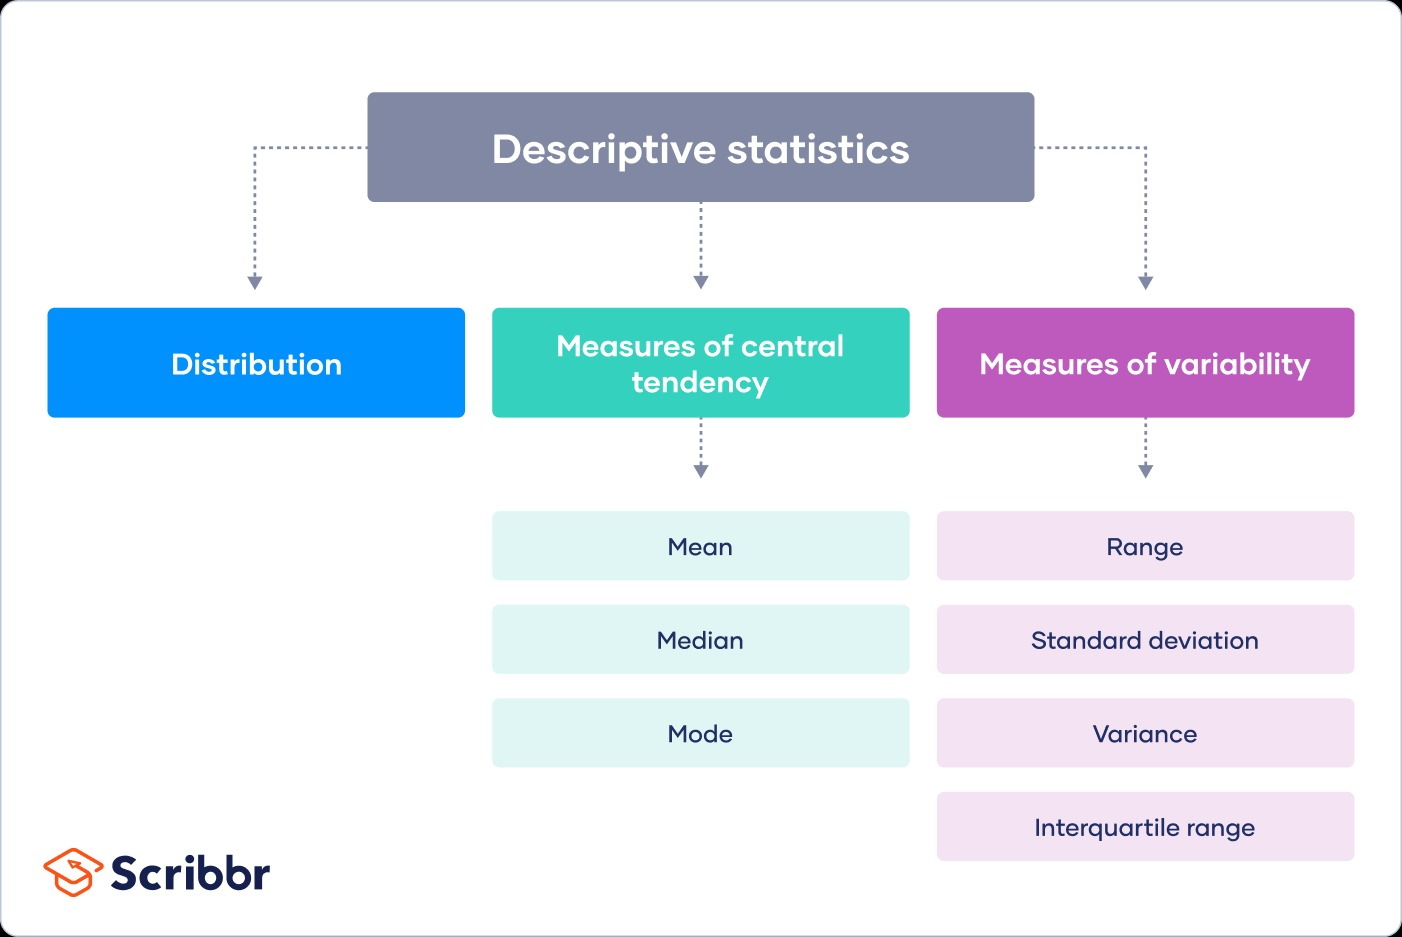
\includegraphics[width=1\textwidth,height=\textheight]{images/desc_stats.jpg}}

\hypertarget{distribution-1}{%
\subsection*{Distribution}\label{distribution-1}}
\addcontentsline{toc}{subsection}{Distribution}

fill

\hypertarget{simple}{%
\subsubsection*{Simple}\label{simple}}
\addcontentsline{toc}{subsubsection}{Simple}

fill

\hypertarget{grouped}{%
\subsubsection*{Grouped}\label{grouped}}
\addcontentsline{toc}{subsubsection}{Grouped}

fill

\hypertarget{central-tendency}{%
\subsection*{Central Tendency}\label{central-tendency}}
\addcontentsline{toc}{subsection}{Central Tendency}

fill

\hypertarget{mean}{%
\subsubsection*{Mean}\label{mean}}
\addcontentsline{toc}{subsubsection}{Mean}

fill

\hypertarget{median}{%
\subsubsection*{Median}\label{median}}
\addcontentsline{toc}{subsubsection}{Median}

fill

\hypertarget{mode}{%
\subsubsection*{Mode}\label{mode}}
\addcontentsline{toc}{subsubsection}{Mode}

fill

\hypertarget{variability}{%
\subsection*{Variability}\label{variability}}
\addcontentsline{toc}{subsection}{Variability}

fill

Range Standard Deviation Variance

fill

\hypertarget{inferential-statistics}{%
\section{Inferential Statistics}\label{inferential-statistics}}

fill

\hypertarget{t-tests}{%
\subsection*{t-tests}\label{t-tests}}
\addcontentsline{toc}{subsection}{t-tests}

fill

\hypertarget{anovas}{%
\subsection*{ANOVAs}\label{anovas}}
\addcontentsline{toc}{subsection}{ANOVAs}

fill

\hypertarget{regressions}{%
\subsection*{Regressions}\label{regressions}}
\addcontentsline{toc}{subsection}{Regressions}

fill

\hypertarget{appendix}{%
\chapter{Appendix}\label{appendix}}

\hypertarget{assignments}{%
\section{Assignments}\label{assignments}}

\hypertarget{individual}{%
\subsection*{Individual}\label{individual}}
\addcontentsline{toc}{subsection}{Individual}

\hypertarget{welcome-post}{%
\subsubsection*{Welcome Post}\label{welcome-post}}
\addcontentsline{toc}{subsubsection}{Welcome Post}

Because this course has a final team project that requires a significant amount of work, it is best to get started early. To assist with this, the first assignment is a welcome post. Within this course on Blackboard, you must post a welcome post. In this welcome post, include an image of yourself and answers to the following questions.

\begin{enumerate}
\def\labelenumi{\arabic{enumi}.}
\tightlist
\item
  What is your name?
\item
  Where are you from?
\item
  What is your desired career?
\item
  What is your favorite hobby?
\item
  What is your biggest pet peeve?
\item
  What is your favorite media properties to consume (e.g., \emph{The West Wing,} \emph{One Punch Man}, \emph{Call of Duty}, \emph{Harry Potter})?
\item
  What would you like to study this semester? (\emph{this can be specific or broad})
\end{enumerate}

\hypertarget{irb-certification}{%
\subsubsection*{IRB Certification}\label{irb-certification}}
\addcontentsline{toc}{subsubsection}{IRB Certification}

Be sure to complete the~\href{https://www.citiprogram.org/Shibboleth.sso/Login?target=https\%3A\%2F\%2Fwww.citiprogram.org\%2FSecure\%2FWelcome.cfm?inst=551\&entityID=https\%3A\%2F\%2Fsts.windows.net\%2F99f37d21-0b5c-43ea-9103-e16f02f5aecf\%2F}{CITI training}.

\hypertarget{apa-assignment}{%
\subsubsection*{APA Assignment}\label{apa-assignment}}
\addcontentsline{toc}{subsubsection}{APA Assignment}

Please provide accurate APA Reference List citations for the references provided on Blackboard in a .docx file. Please submit as a .doc or .docx file. Be sure to follow APA 7th Edition rules.

\hypertarget{annotated-bibliography}{%
\subsubsection*{Annotated Bibliography}\label{annotated-bibliography}}
\addcontentsline{toc}{subsubsection}{Annotated Bibliography}

Individuals are tasked with submitting a set of four (4) annotated bibliographies that are potentially relevant to their paper. Individuals are to submit unique annotated bibliographies. This means that if you and your team members collaborate on finding sources, you each must annotate different sources.. I recommned at least being from an academic paper or reputible scholarly book (preference toward paper).

I will attach a word document with formatting and content suggestions to this assignment.

\hypertarget{visualization-assignment}{%
\subsubsection*{Visualization Assignment}\label{visualization-assignment}}
\addcontentsline{toc}{subsubsection}{Visualization Assignment}

The visualization assignment will be posted as an .Rmd file on Blackboard. You are expected to create a new R Project for this assignment and then submit the zipped project on Blackboard. You may work on this as a group; however, I expect your visualizations to be moderately unique. \textbf{Do not plagiarize!}

\hypertarget{analysis-assignment}{%
\subsubsection*{Analysis Assignment}\label{analysis-assignment}}
\addcontentsline{toc}{subsubsection}{Analysis Assignment}

The analysis assignment will be posted as an .Rmd file on Blackboard. You are expected to create a new R Project for this assignment and then submit the zipped project on Blackboard. Each analysis question will require the code to run the analysis and your individual interpretation. You may work on this as a group; however, I expect your interpretation to be in your own words. \textbf{Do not plagiarize!}

\hypertarget{section-quizzes}{%
\subsubsection*{Section Quizzes}\label{section-quizzes}}
\addcontentsline{toc}{subsubsection}{Section Quizzes}

I will divide your book into five (5) sections and create five (5) minor quizzes. These quizzes will be posted around midterm. You will then have until the last week of class (before final's week) to submit all the quizzes.

\hypertarget{team}{%
\subsection*{Team}\label{team}}
\addcontentsline{toc}{subsection}{Team}

\hypertarget{partner-contract}{%
\subsubsection*{Partner Contract}\label{partner-contract}}
\addcontentsline{toc}{subsubsection}{Partner Contract}

I will attach a word document on Blackboard as a template partner contract. All team members must sign before submission.

\textbf{Common Tasks (\emph{suggestions)}\\
}Outliner\\
Reference Manager\\
Run analyses (in R)\\
Create visualizations (in R)\\
Reference Summarizer\\
Presenter\\
Lead Writer for Section (\href{https://psychology.ucsd.edu/_files/undergrad/writingresearchpapersinapastyleguide.pdf}{How to Write APA Style Research Papers})

\begin{enumerate}
\def\labelenumi{\arabic{enumi}.}
\item
  Introduction
\item
  Literature Review
\item
  Methodology
\item
  Results
\item
  Discussion
\item
  Conclusion
\end{enumerate}

\hypertarget{topic-selection}{%
\subsubsection*{Topic Selection}\label{topic-selection}}
\addcontentsline{toc}{subsubsection}{Topic Selection}

Submit your topic selection, including potential theories and rough research hypotheses or questions.

You can find theories in the theories chapter.

\emph{\textbf{Example}: We plan to survey students to identify a correlation between media usage and satisfaction. Borrowing from uses and gratification theory (though our theory choice may change as we spend more time reading), we expect individuals to select their media based upon the needs they are attempting to fulfill. Types of media include traditional (e.g., television, movies) and new (e.g., TikTok, YouTube). We are interested in if any usage impacts quality of life and if quantity of usage controls for some variation. If we receive a diverse enough participant pool, we are also interested in home type (i.e., single, family {[}as child{]}, friends, partner, family {[}as parent{]}). Our interest in home type is a reflection of the pandemic's limiting of outside interaction.}

\hypertarget{irb-application}{%
\subsubsection*{IRB Application}\label{irb-application}}
\addcontentsline{toc}{subsubsection}{IRB Application}

Each student must submit proof of IRB application submission. Each team \textbf{must} add me to their application so that I can access the material. You are graded on submitting a full application on time and how few revisions are required to pass. \ul{\textbf{Please reach out to me before}} submission so I can advise you on your project and accuracy.

\hypertarget{research-questionshypotheses}{%
\subsubsection*{Research Questions/Hypotheses}\label{research-questionshypotheses}}
\addcontentsline{toc}{subsubsection}{Research Questions/Hypotheses}

You are to present at least two (2) \textbf{concise} research questions (RQ) or hypotheses (RH) that your team want to examine. These RQs/RHs must include at least one (1) independent variable and one (1) dependent variable. These variables must be measurable for your project. If you have questions, please reach out before this assignment is due.

\hypertarget{research-proposal}{%
\subsubsection*{Research Proposal}\label{research-proposal}}
\addcontentsline{toc}{subsubsection}{Research Proposal}

Your research proposal is intended to be your first three (3) sections of your research paper: literature review, research objective, and methods. The proposal does not have to be a perfect version of these sections; however, the closer these are to complete, the work your team will have later in the semester.

I will post more specifics on Blackboard during the semester.

\hypertarget{outline}{%
\subsubsection*{Outline}\label{outline}}
\addcontentsline{toc}{subsubsection}{Outline}

Your outline is intended to give me a sneak peak of where you stand with your final three (3) sections of your research paper (i.e., results, discussion, and conclusion) before your final paper is due. The outline must be in numbers/bulleted format and not paragraph. The text in the outline can either be small phrases or full sentences. This is your final chance for feedback before you focus down on your final project.

\hypertarget{full-paper}{%
\subsubsection*{Full Paper}\label{full-paper}}
\addcontentsline{toc}{subsubsection}{Full Paper}

At the completion of this course, all student will have to submit a full research paper with their teams. Specifics will be presented throughout the semester.

\hypertarget{presentation}{%
\subsubsection*{Presentation}\label{presentation}}
\addcontentsline{toc}{subsubsection}{Presentation}

To accompany your final paper, your group is required to present your paper. Not all members have to present; however, this relies on your partner contract.

The presentation will be done during our scheduled time for our final (December 12, 10-11:40 am).~

\begin{itemize}
\item
  7-10 minutes
\item
  Powerpoint
\item
  Include key sections (Literature, RQ/RH, Methods, Results, Discussion)
\item
  Provide context
\end{itemize}

Beyond that, your presentation is up to you.

Submit your PowerPoint slides on Blackboard. You must also submit your partner contract with any important changes and commentary to reflect an imbalance in workload.

  \bibliography{book.bib,packages.bib}

\end{document}
